\part{Trigonometría y Complejos}



\null\vfill
\begin{Huge}\begin{center}
II. Trigonometría y Complejos
\end{center}\end{Huge}

\vspace{1.5cm}

\begin{figure}[H]
	\centering
	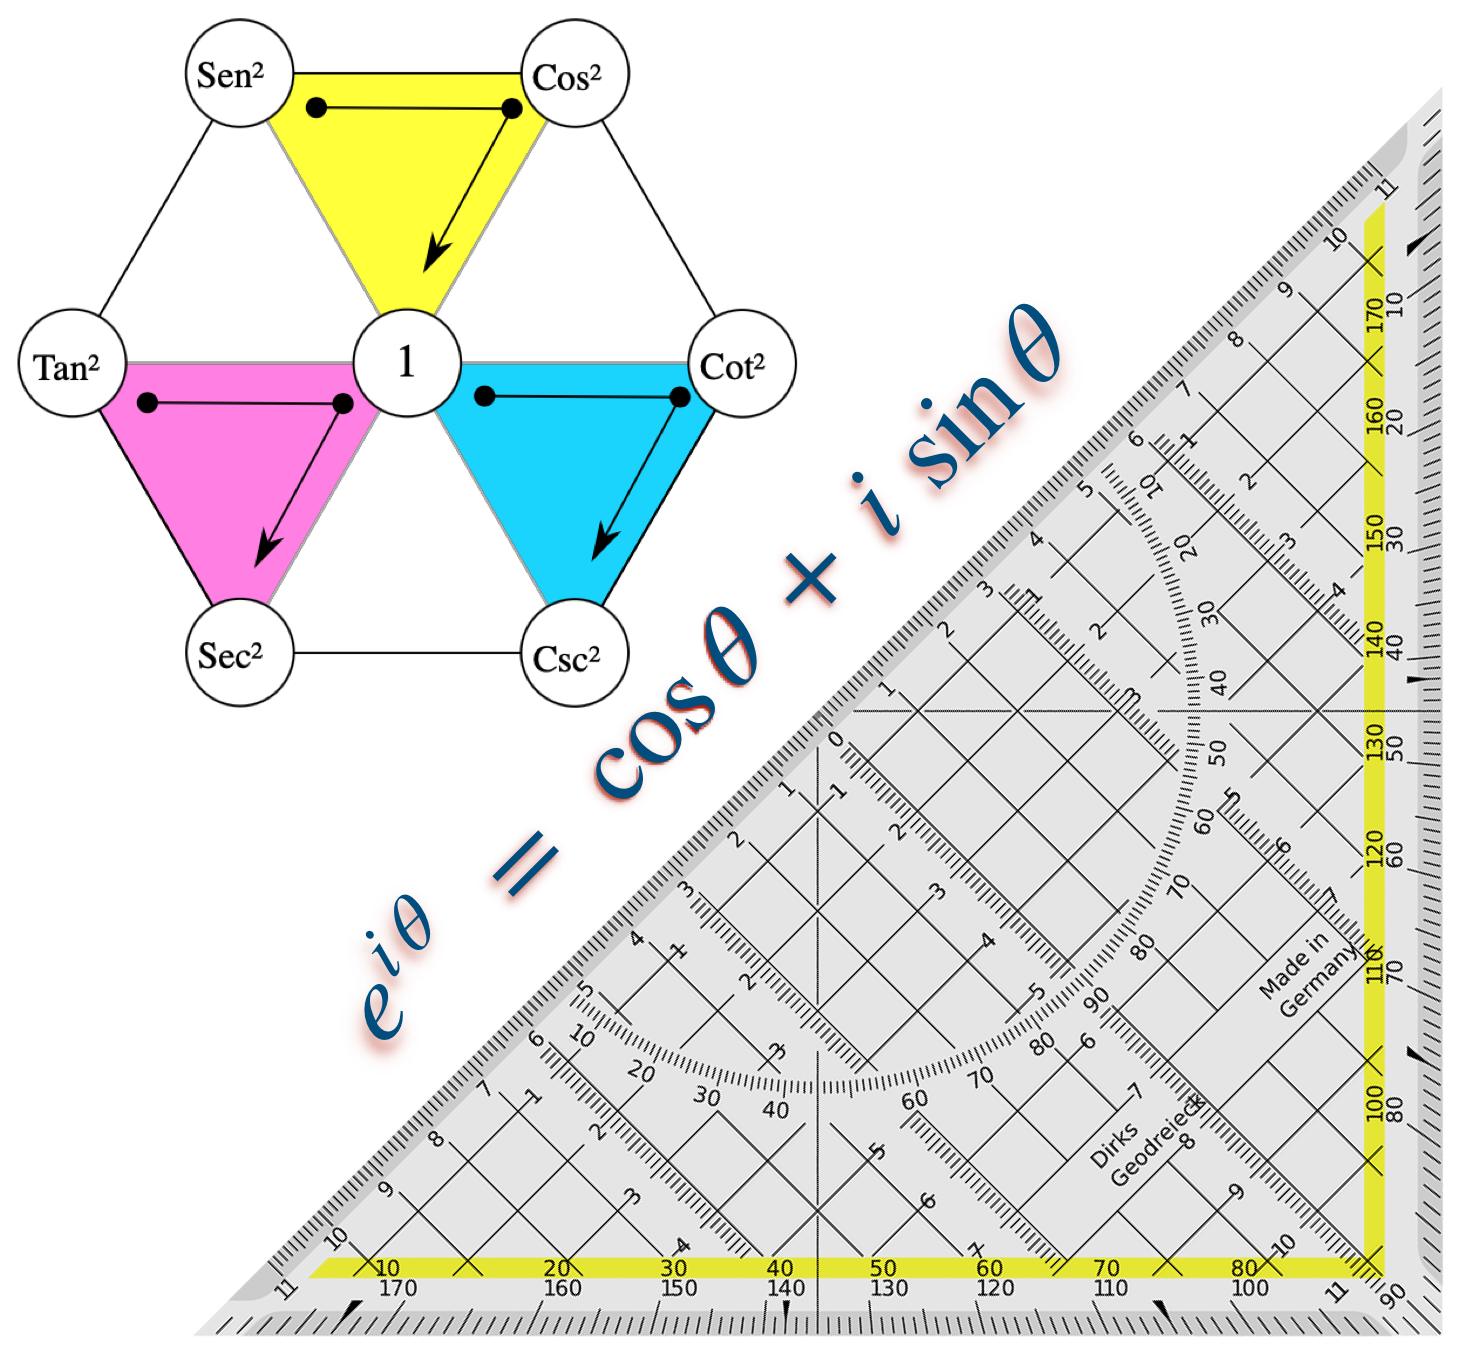
\includegraphics[width=.6\textwidth]{imagenes/part2.png}	
\end{figure}
\par
\vfill



\chapter{Razones trigonométricas}

\begin{tikzpicture}
	\fill [left color=red!50, right color=teal!50] (0,0) rectangle (6.5,.2);
	\fill [left color=teal!50, right color=blue!50] (6.5,0) rectangle (11.5,.2);
	\end{tikzpicture}

\vspace{10mm}


\begin{adjustwidth}{30pt}{30pt}
\begin{cuadro-gris}

	\begin{multicols}{2}
	En este tema se repasan de los conceptos estudiados en cursos anteriores.
	
	$\triangleright \quad$  Razones trigonométricas (RT) de ángulos agudos.
	
	$\triangleright \quad$  RT Ángulos notables.
	
	$\triangleright \quad$  Extensión RT a ángulos cualesquiera.
	
	$\triangleright \quad$  Ángulos complementarios, suplementarios y opuestos.
	
	$\triangleright \quad$ Funciones trigonométricas.
	
	$\triangleright \quad$ Identidades y ecuaciones trigonométricas.
	
	$\triangleright \quad$ Resolución de triángulos rectángulos.
	\end{multicols}
	
\end{cuadro-gris}
\end{adjustwidth}

\vspace{5mm}

\begin{myexampleblock}{Trigonometría}
\vspace{2mm} La trigonometría es una rama de la matemática cuyo significado etimológico es `la medición de los triángulos'. 
Deriva de los términos griegos \emph{trigonos} (triángulo) y \emph{metrón} (medida).


\vspace{2mm} En términos generales, la trigonometría es el estudio de las razones trigonométricas: seno, coseno, tangente, cotangente, secante y cosecante. La trigonometría se aplica a otras ramas de la geometría o la geometría analítica en particular geometría plana o geometría del espacio.

\vspace{2mm} Posee numerosas aplicaciones, entre las que se encuentran: las técnicas de triangulación (usadas en astronomía para medir distancias a estrellas próximas), en la medición de distancias entre puntos geográficos (topografía), y en sistemas globales de navegación por satélites (GPS).	



\vspace{2mm} Los egipcios, en el segundo milenio antes de Cristo, utilizaban una forma primitiva de la trigonometría, para la construcción de las pirámides. El \emph{Papiro de Ahmes}, escrito por el escriba egipcio Ahmes (1680 a.C.-1620 a.C.), contiene el siguiente problema relacionado con la trigonometría:

\vspace{2mm}Si una pirámide es de 250 codos de alto y el lado de su base es de 360 codos de largo, ?`cuál es su Seked?\footnote{ Seked: medida de la inclinación de las caras de una pirámide, equivalente actual a  $51^0 50' 35"$. }

\begin{multicols}{2}
\vspace{2mm}La solución al problema es la relación entre la mitad del lado de la base de la pirámide y su altura. En otras palabras, la medida que se encuentra para la seked será lo que llamaremos  \emph{cotangente} del ángulo que forman la base de la pirámide y su respectiva cara.
\begin{figure}[H]
	\centering
	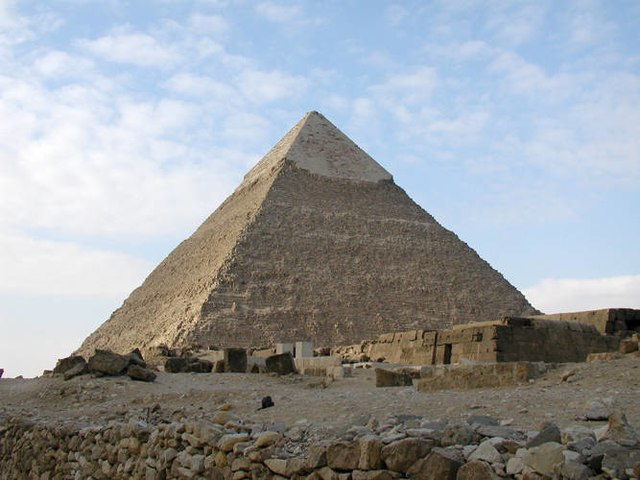
\includegraphics[width=0.35\textwidth]{img-rt/rt01.jpg}
\end{figure}
\end{multicols}
\end{myexampleblock}



\vspace{0.5cm}
\section{Medida de ángulos}
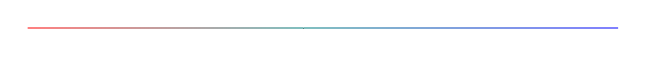
\begin{tikzpicture}
	\fill [left color=red!50, right color=teal!50] (0,0) rectangle (3.5,.01);
	\fill [left color=teal!50, right color=blue!50] (3.5,0) rectangle (7.5,.01);
	\end{tikzpicture}
\vspace{0.5cm}


\begin{definition}

En geometría, el ángulo puede ser definido como la parte del plano determinada por dos semirrectas llamadas lados que tienen el mismo punto de origen llamado vértice del ángulo. 
\begin{multicols}{2}
La medida de un ángulo es considerada como la amplitud del arco de circunferencia centrada en el vértice y delimitada por sus lados. Su medida es un múltiplo de la razón entre la longitud del arco y el radio. Su unidad natural es el \emph{radián}, pero también se puede utilizar el \emph{grado sexagesimal}.
\begin{figure}[H]
	\centering
	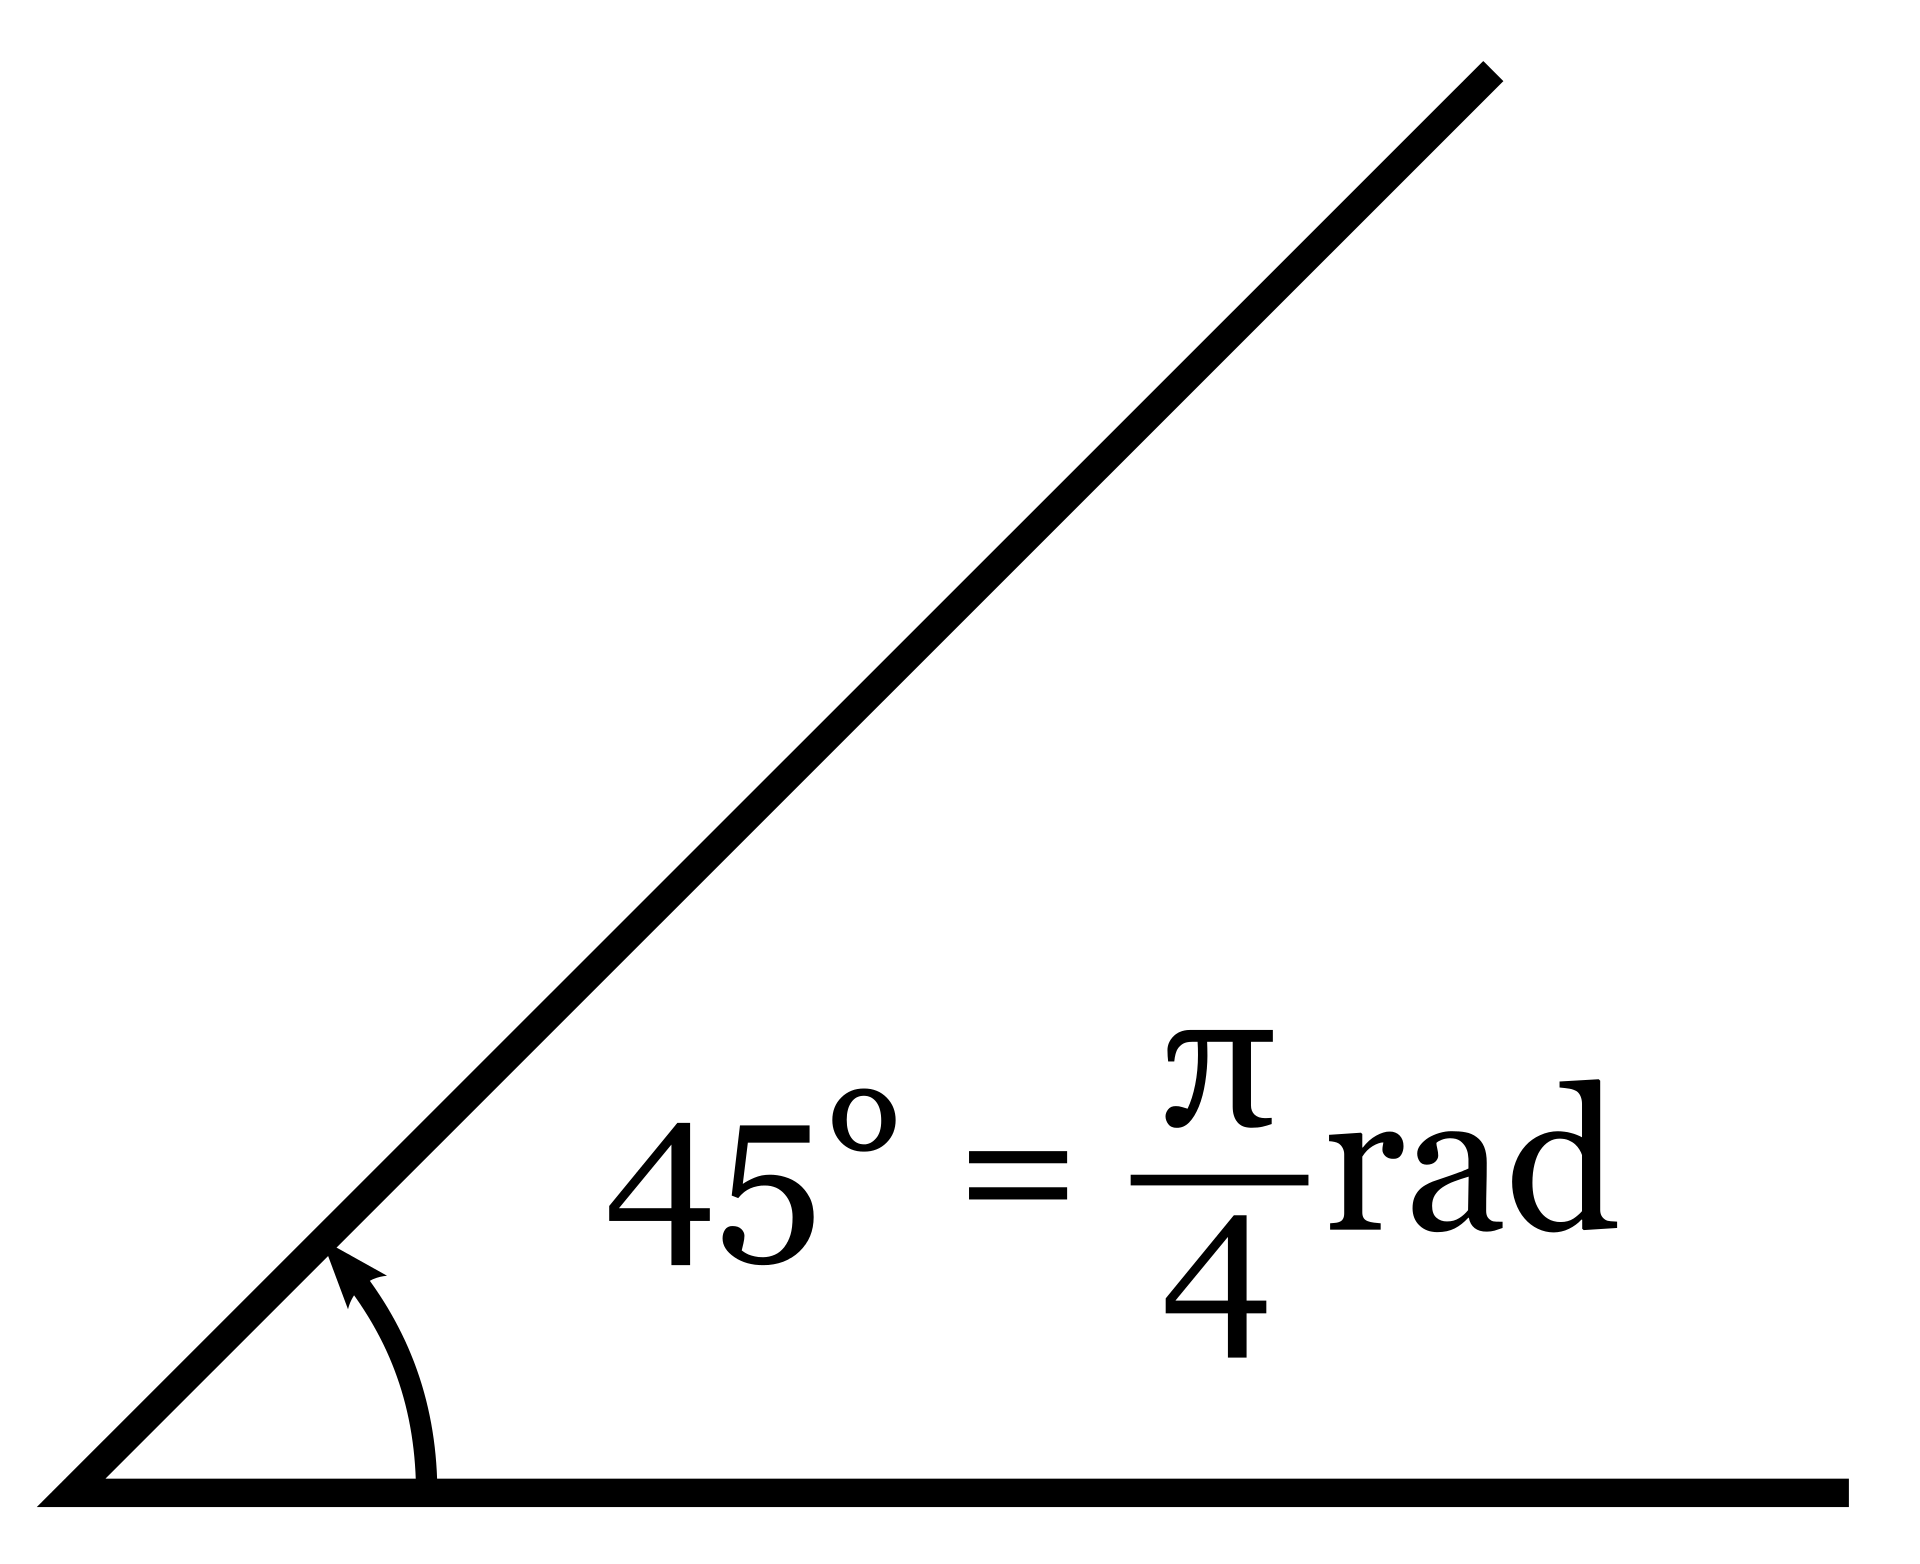
\includegraphics[width=0.3\textwidth]{img-rt/rt02.png}
\end{figure}
\end{multicols}

En matemáticas  los ángulos se calculan siempre en sentido contrario a las agujas del reloj, sentido positivo. Un ángulo medido en sentido contrario se considera negativo.
\end{definition}

\vspace{5mm}
\begin{definition}[ Radián]
	. Un \textbf{radián} es el ángulo que subtiende un radio, es decir, es aquel ángulo de la circunferencia cuyo arco mide exactamente lo mismo que el radio.
\end{definition}

Puesto que el arco de toda la circunferencia ($360^o$) mide $2\pi r$, el número de radianes de una \emph{ángulo completo} es de $\dfrac{2\pi r}{r} \ = \ \boldsymbol{ 2\pi }$ radianes.

Para pasar de grados sexagesimales a radianes o viceversa podemos hacer uso de los factores de conversión. Según acabamos de ver, un ángulo completo son $2\pi$ rad que equivalen a $360^o$, el factor de conversión a usar es pues  $\ \dfrac{2\pi \, \mathrm{rad}}{360^o}= \dfrac{\pi}{180}\ \mathrm{rad} / \mathrm{grado}$, para pasar de grados o radianes; o el factor inverso $\ \dfrac{180}{\pi} \ \mathrm{grado}/\mathrm{rad}$, para pasar de radianes a grados.  

\begin{figure}[H]
	\centering
	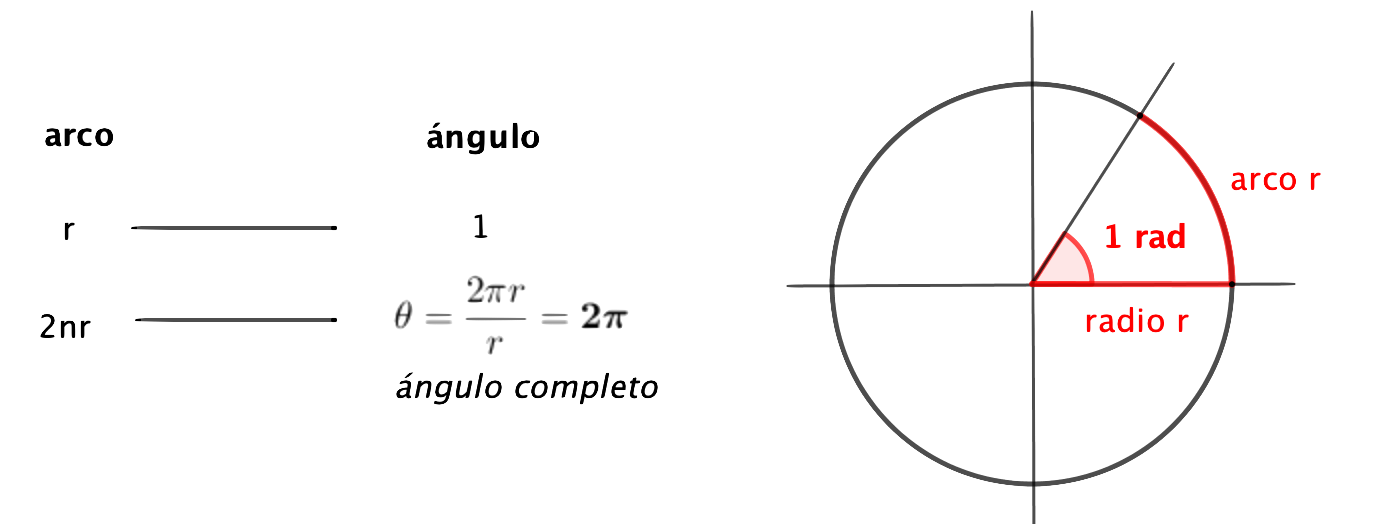
\includegraphics[width=0.85\textwidth]{img-rt/rt03.png}
\end{figure}

\textcolor{gris}{Los radianes (los ángulos en general) son una medida adimensional, ya que $1\, \mathrm{rad} =\dfrac{s=1\, \mathrm{m}}{r=1\, \mathrm{m}}$, no tiene dimensiones. De todos modos, para indicar en que unidad lo medimos, cuando demos un ángulo explicitaremos en que unidad lo hacemos.}


\begin{multicols}{2}

$\,$

Si el ángulo está medido en radianes, es cierta la relación:

$\,$

arco = ángulo $\times $ radio
$\qquad \boldsymbol{ s\ = \ \alpha \ \times \ r }$

\begin{figure}[H]
	\centering
	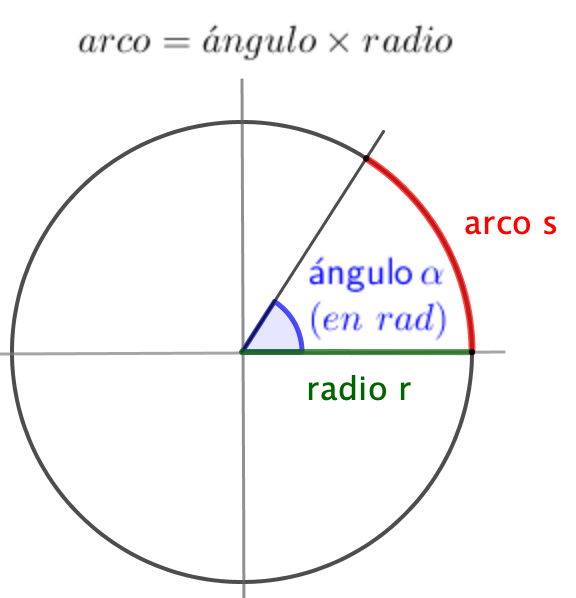
\includegraphics[width=0.3\textwidth]{img-rt/rt04.png}
\end{figure}	
\end{multicols}

\begin{miejemplo}
. Expresa en radianes: $\ 30^o,\quad 45^o,\quad 60^o,\quad 225^o,\quad 300^o, \quad 1^o$

\vspace{2mm} Expresa en grados: $\ 1 \, \mathrm{rad},\quad 7\pi/4 \, \mathrm{rad},\quad 5 \, \mathrm{rad}$

\vspace{5mm}

\begin{multicols}{3}
\vspace{2mm}$30^o=30 \dfrac{\pi}{180}=\dfrac \pi 6 \, \mathrm{rad}$

\vspace{2mm}$45^o=45 \dfrac{\pi}{180}=\dfrac \pi 4 \, \mathrm{rad}$

\vspace{2mm}$60^o=60 \dfrac{\pi}{180}=\dfrac \pi 3 \, \mathrm{rad}$

\vspace{2mm}$225^o=225 \dfrac{\pi}{180}=5\dfrac \pi 4 \, \mathrm{rad}$

\vspace{2mm}$300^o=300 \dfrac{\pi}{180}=5\dfrac \pi 3 \, \mathrm{rad}$

\vspace{2mm}$1^o=1 \dfrac{\pi}{180}=\dfrac \pi {180} \, \mathrm{rad}$

\vspace{2mm}$1\, \mathrm{rad}=1 \dfrac{180}{\pi}=57.296^o$

\vspace{2mm}$7\dfrac \pi 4 \, \mathrm{rad}=7\dfrac \pi 4 \dfrac{180}{\pi}=325^o$

\vspace{2mm}$5\, \mathrm{rad}=5 \dfrac{180}{\pi}=286.479^o$

\end{multicols}
\end{miejemplo}

\begin{miejercicio}

?`Cuántos radianes suman los ángulos de un triángulo? ?`Qué mide un ángulo recto en radianes?

\rule{250pt}{0.1pt}
\vspace{5mm}

Ángulos de un triángulo suman $180^o=180 \dfrac{\pi}{180}=\pi \, \mathrm{rad}$

\vspace{2mm}Ángulo recto $\ 90^o=90  \dfrac{\pi}{180}=\dfrac\pi 2 \, \mathrm{rad}$
	
\end{miejercicio}


\begin{miejercicio}
. Si se recorren 3 rad en una circunferencia de 2 m, ?`cuánto espacio se ha recorrido? ¿Y si se recorren $70^o$?

\rule{250pt}{0.1pt}
\vspace{5mm} 

arco=ángulo $\times$ radio ($s=\alpha \cdot r$), siempre que el ángulo esté expresado en radianes.

\vspace{2mm} $\alpha=3 \, \mathrm{rad}, \ r=2 \, \mathrm{m} \ \quad \ s=3\cdot 2 =6  \, \mathrm{m}$

\vspace{2mm} $\alpha=70^o=70 \dfrac{\pi}{180} \, \mathrm{rad}, \ r=2 \, \mathrm{m} \ \quad \ s= 70 \dfrac{\pi}{180} \cdot 2 =7\dfrac \pi 9 =2.443  \, \mathrm{m}$
	
\end{miejercicio}



\vspace{0.5cm}
\section[Razones trigonométricas de ángulos agudos. Relación fundamental de la trigonometría]{Razones trigonométricas de ángulos agudos. Relación fundamental de la trigonometría\sectionmark{RT ángulos agudos}}
\sectionmark{RT ángulos agudos}
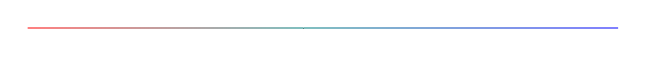
\begin{tikzpicture}
	\fill [left color=red!50, right color=teal!50] (0,0) rectangle (3.5,.01);
	\fill [left color=teal!50, right color=blue!50] (3.5,0) rectangle (7.5,.01);
	\end{tikzpicture}
\vspace{0.5cm}


\begin{definition}[ seno - coseno - tangente]

En cualquier triángulo rectángulo, elegido uno de sus ángulos agudos, se definen el seno, coseno y tangente como:

\begin{multicols}{2}

$$\sin \alpha \ = \ \dfrac{\mathrm{cateto \ opuesto}}{\mathrm{hipotenusa}} \ = \ \dfrac y r$$

$$\cos \alpha \ = \ \dfrac{\mathrm{cateto \ contiguo}}{\mathrm{hipotenusa}} \ = \ \dfrac x r$$

$$\tan \alpha \ = \ \dfrac{\sin \alpha}{\cos \alpha} \  =\ \dfrac{\mathrm{cateto \ opuesto}}{\mathrm{cateto \ contiguo}} \ = \ \dfrac y x$$

	\begin{figure}[H]
	\centering
	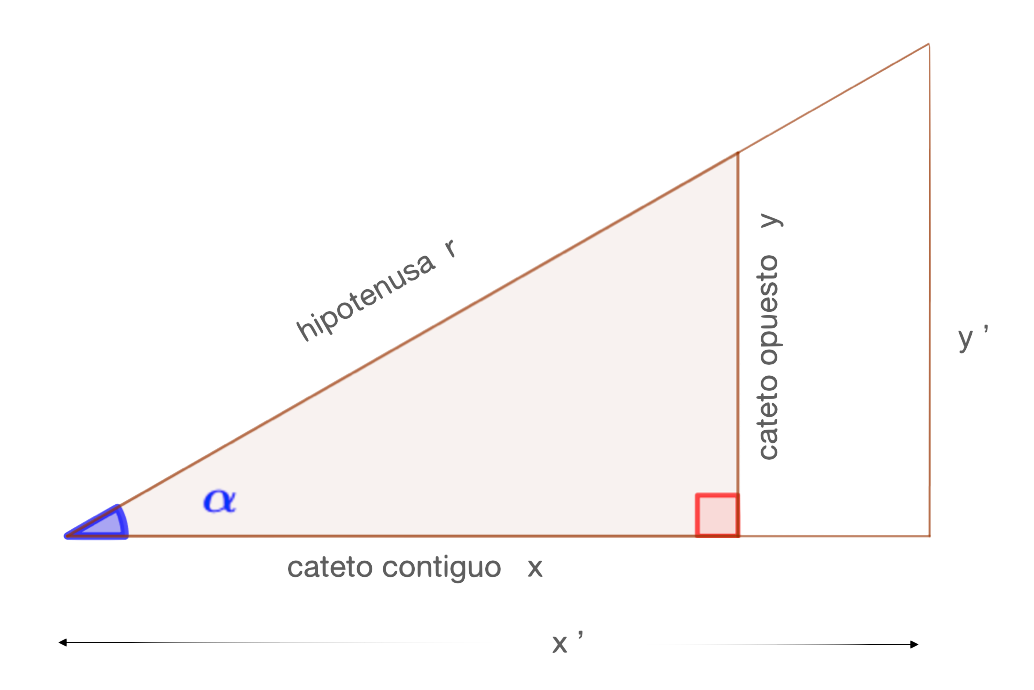
\includegraphics[width=0.5\textwidth]{img-rt/rt05.png}
\end{figure}
\end{multicols}

\end{definition}


En la figura puede observarse, en virtud del teorema de Thales, que las razones trigonométricas no dependen del triángulo elegido, solamente del ángulo considerado, p.e. $\ \frac {y'}{x'}=\frac y x =\tan \alpha$. 


\vspace{2mm} También se definen las siguientes tres razones tigonométricas derivadas de las anteriores: secante, cosecante y cotangente.


$$\sec \alpha \ = \ \dfrac 1{\cos \alpha}\, ; \qquad \csc \alpha \ = \ \dfrac 1 {\sin \alpha} \, ; \qquad \cot \alpha \ = \ \dfrac 1 {\tan \alpha} \ = \ \dfrac{\cos \alpha}{\sin \alpha}$$


\vspace{2mm} \textcolor{gris}{Se ha optado por nombrar a las razones trigonométricas del modo internacionalmente aceptado, usando solo tres letras para cada una de ella. También es frecuente encontrar expresiones como $\ \mathrm{tg,\ cotg,\ cosec}$}.

\vspace{5mm}
\subsection{Relación fundamental de la trigonometría}
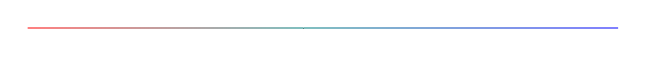
\begin{tikzpicture}
	\fill [left color=red!50, right color=teal!50] (0,0) rectangle (3.5,.01);
	\fill [left color=teal!50, right color=blue!50] (3.5,0) rectangle (7.5,.01);
	\end{tikzpicture}
\vspace{0.5cm}


\begin{theorem}[ Relación fundamental de la trigonometría]

No es más que el teorema de Pitágoras expresado trigonométricamente:


\vspace{2mm} $x^2+y^2=r^2 \ \to \dfrac{x^2}{r^2}+\dfrac{y^2}{r^2}=\dfrac{r^2}{r^2}=1 \ \to \ \left( \dfrac x r \right)^2+\left( \dfrac y r \right)^2= 1 \ \Rightarrow \ \sin^2 \alpha + \cos^2 \alpha = 1$ 
$$\large{
\subrayado{\boxed{\  \boldsymbol{ \
\sin^2 \alpha \ + \  \cos^2 \alpha \ = \ 1
\ } \ }}} \quad \to \quad
\begin{cases} 
\ \sin^2 \alpha = 1-\cos^2 \alpha &\to \ \sin \alpha = \sqrt{1-\cos^2 \alpha}
\\ \\
\ \cos^2 \alpha = 1-\sin^2 \alpha	 &\to \ \cos \alpha = \sqrt{1-\sin^2 \alpha}
\end{cases}
$$

\end{theorem}

\begin{multicols}{2}
$\quad$ 

\textcolor{gris}{En estas expresiones $\sin^2 \alpha$ representa al $(\sin \alpha)^2$, igualmente, $\cos^2 \alpha =(\cos \alpha)^2$}

\begin{figure}[H]
	\centering
	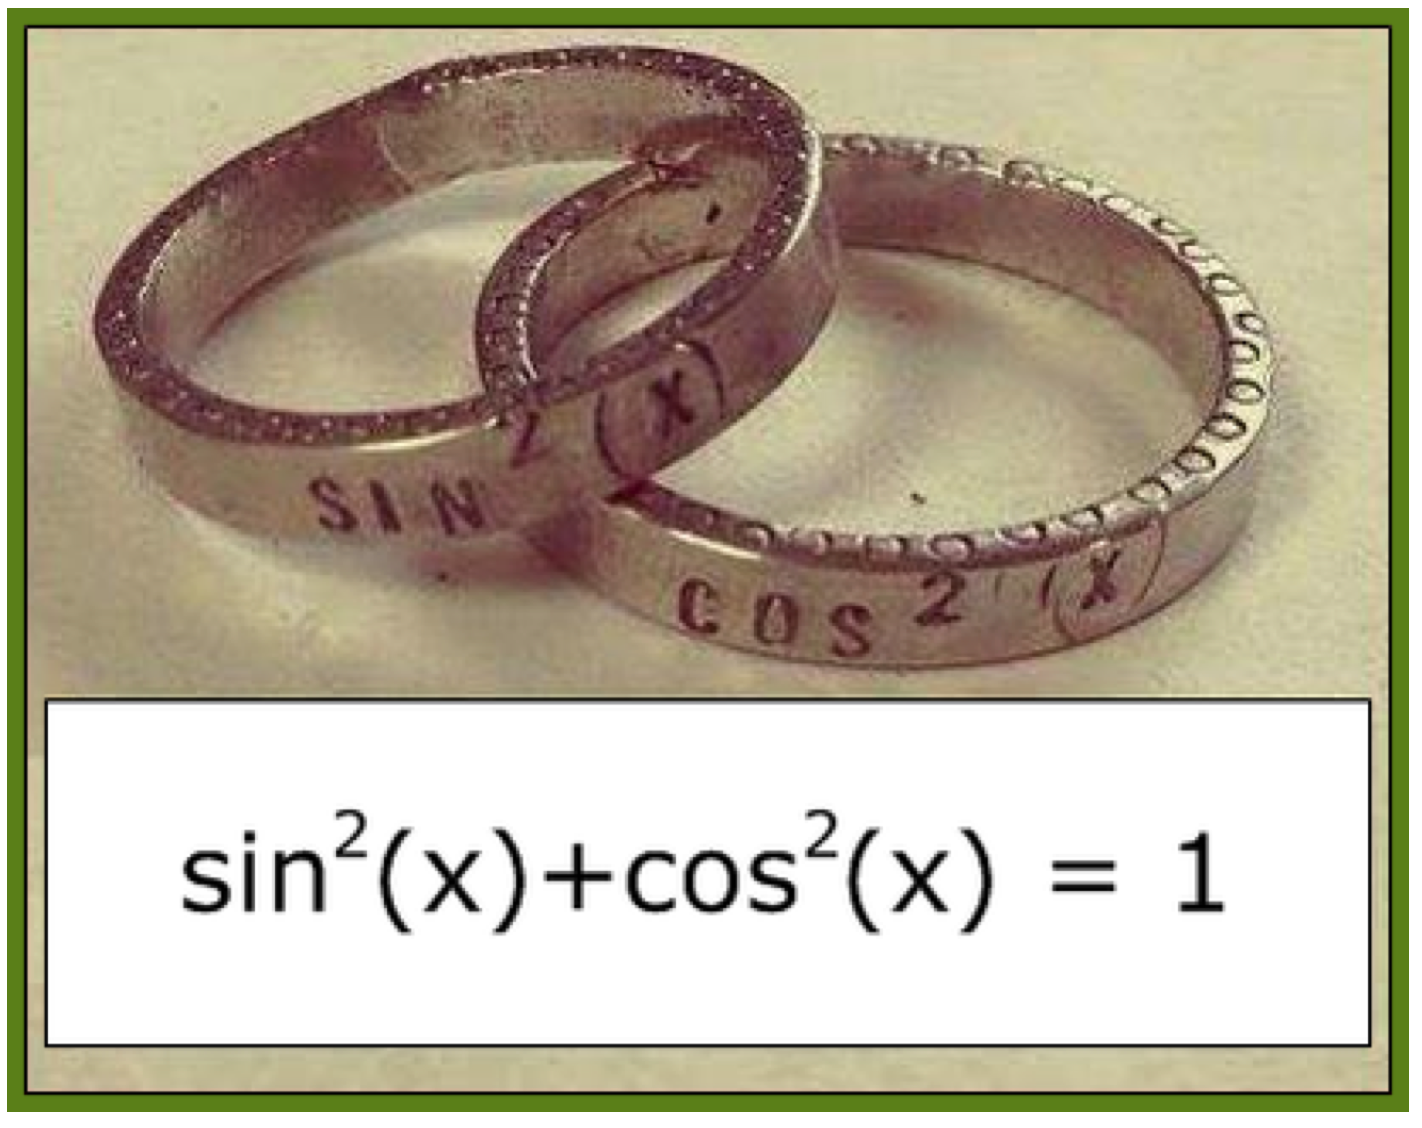
\includegraphics[width=0.25\textwidth]{img-rt/rt24.png}
\end{figure}
\end{multicols}

\vspace{2mm} \begin{theorem} [Otras relaciones fundamentales]
 
 Derivadas de la relación fundamental, se tienen:
 
 $$
 \boldsymbol{
 \sec^2 \alpha \ = \ 1 +\  \tan^2 \alpha \, ; \qquad \qquad \qquad \csc^2 \alpha \ = \  1 \ + \ \cot^2 \alpha
 } $$	
 \end{theorem}

\underline{Demostraciones}:

\vspace{2mm} Dividiendo la relación fundamental por $\cos^2 \alpha$:

\vspace{2mm} \hspace{3cm} $\quad \dfrac{\sin^2 \alpha}{\cos^2 \alpha} + \dfrac{\cos^2 \alpha}{\cos^2 \alpha} = \dfrac {1}{\cos^2 \alpha} \quad \to \quad \tan^2 \alpha + 1 = \sec^2 \alpha $ \QED

\vspace{4mm} Dividiendo la relación fundamental por $\sin^2 \alpha$:

\vspace{2mm} \hspace{3cm} $\quad \dfrac{\sin^2 \alpha}{\sin^2 \alpha} + \dfrac{\cos^2 \alpha}{\sin ^2 \alpha} = \dfrac {1}{\sin^2 \alpha} \quad \to \quad 1+\cot^2 \alpha = \csc^2 \alpha $ \QED


\vspace{4mm} Vistas las relaciones trigonométricas observamos que son redundantes: a partir de las relaciones entre ellas y las relaciones fundamentales, con una sola de ellas es suficiente para determinar todas las demás. Pero al estar al cuadrado en las relaciones fundamentales tendremos una doble posibilidad en el signo al extraer la raíz y para determinar con que signo quedarnos necesitamos desarrollar la siguiente sección, \emph{extensión de las razones trigonométricas a cualquier ángulo}, ya que hasta el momento solo las tenemos definidas para ángulos agudos.

\vspace{5mm}
\subsection{Razones trigonométricas de ángulos notables} 
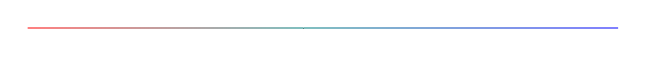
\begin{tikzpicture}
	\fill [left color=red!50, right color=teal!50] (0,0) rectangle (3.5,.01);
	\fill [left color=teal!50, right color=blue!50] (3.5,0) rectangle (7.5,.01);
	\end{tikzpicture}
\vspace{0.5cm}

De todos los triángulos rectángulos hay dos especialmente \emph{notables}:

--- la escuadra: triángulo rectángulo e isósceles, ángulos de $45^o = \pi/4$ rad.

--- el cartabón: medio triángulo equilátero, ángulo de $30^o = \pi/6$ rad y $60^o=\pi/3$ rad.

\begin{figure}[H]
	\centering
	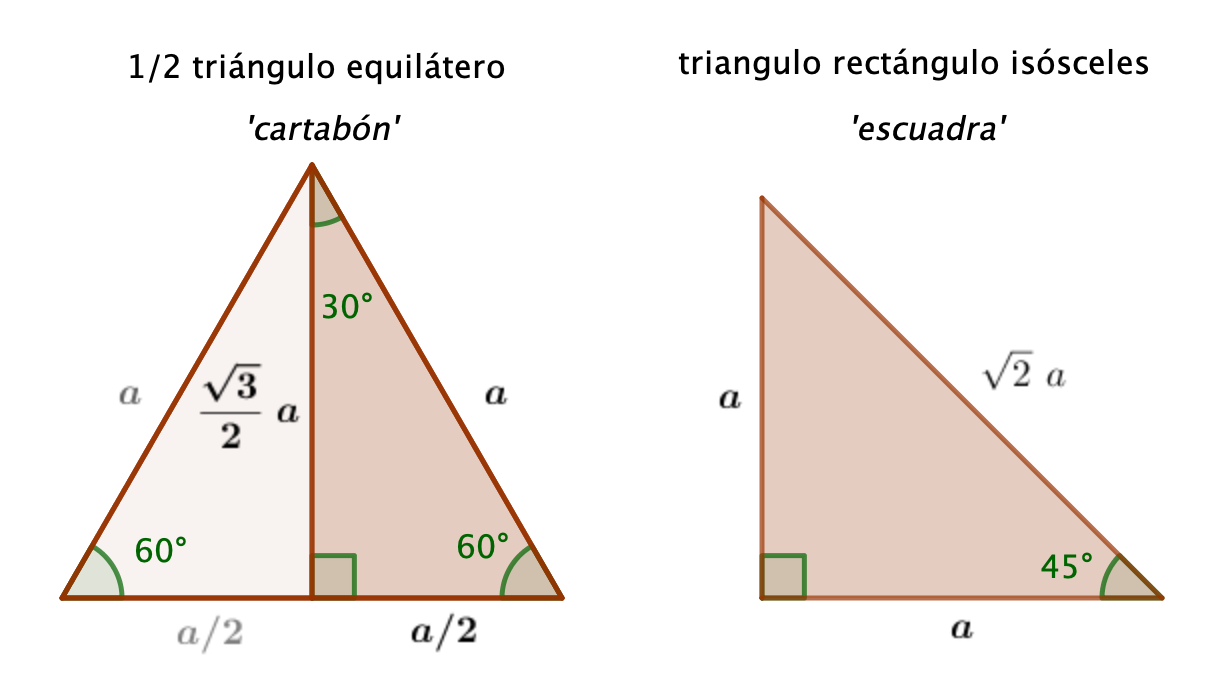
\includegraphics[width=0.7\textwidth]{img-rt/rt06.png}
\end{figure}


Es sencillo comprobar que \textcolor{gris}{(suponer triángulos de lados $a$ y aplicar el teorema de Pitágoras)}:


\vspace{4mm}
\begin{adjustwidth}{50pt}{50pt}
\begin{cuadro-naranja}
\begin{table}[H]
\centering
\begin{tabular}{lllll}
$\sin 30^o = \dfrac 1 2$  & $\qquad$ & $\sin 45^o=\dfrac{\sqrt{2}}{2}$ & $\qquad$  & $\sin 60^o=\dfrac{\sqrt{3}}{2}$ \\
 &  &  &  &  \\
$\cos 30^o=\dfrac{\sqrt{3}}{2}$ &  & $\cos 45^o=\dfrac{\sqrt{2}}{2}$ &  & $\cos 60^o=\dfrac 1 2 $ \\
 &  &  &  &  \\
$\tan 30^o=\dfrac{\sqrt{3}}{3}$ &  & $\tan 45^o=1$ &  & $\tan 60^o=\sqrt{3}$
\end{tabular}
\end{table}
\vspace{-5mm}
\end{cuadro-naranja}
\end{adjustwidth}

\begin{figure}[H]
	\centering
	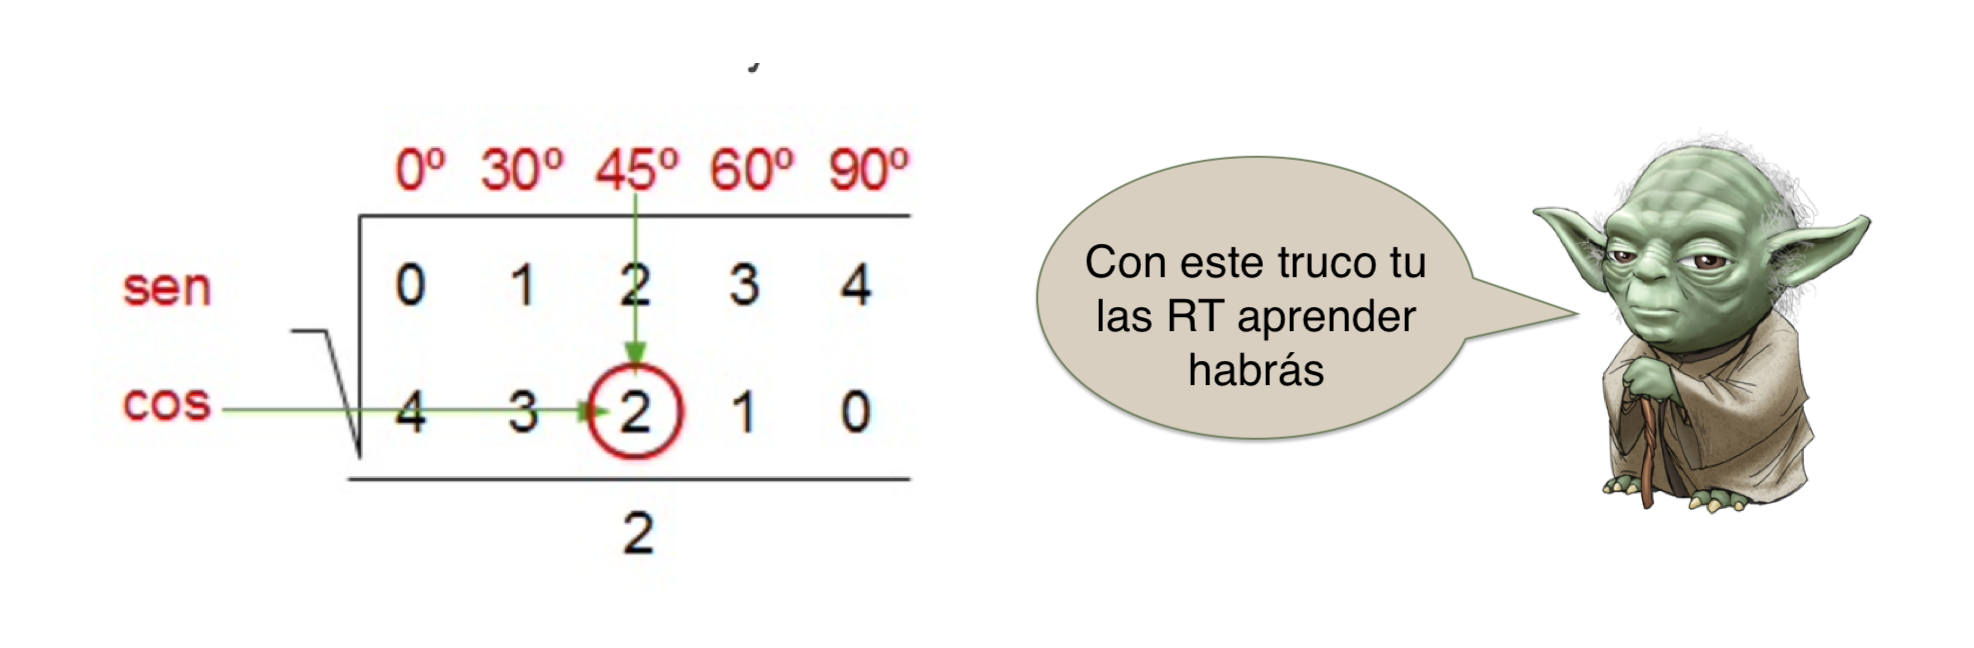
\includegraphics[width=0.8\textwidth]{img-rt/rt48.png}
\end{figure}


\section{Extensión de las RT a cualquier ángulo}
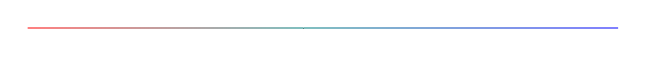
\begin{tikzpicture}
	\fill [left color=red!50, right color=teal!50] (0,0) rectangle (3.5,.01);
	\fill [left color=teal!50, right color=blue!50] (3.5,0) rectangle (7.5,.01);
	\end{tikzpicture}
\vspace{2mm}

Se llama \emph{\textbf{circunferencia goniométrica}} a aquella de radio unidad. Mediremos los ángulos desde el semieje $X$ positivo en sentido \emph{levógiro}, contrario a las agujas del reloj. Los ángulos medidos en el sentido de las agujas del reloj (\emph{dextrógiro}) se considerarán ángulo negativos.

Cualquier ángulo agudo $(0<\alpha<90^o)$ se representará por un punto de coordenadas $(x,y)$ en la circunferencia. La proyección sobre el eje $X$ de este punto, junto con el origen, forman un triángulo que siempre será rectángulo (por construcción) y de hipotenusa $1$, por ello, tendremos que $\ \sin \alpha =\dfrac y 1 =y;\ \cos \alpha=\dfrac x 1 = x$. El seno vendrá medido por la proyección vertical (rojo) y el coseno por la horizontal (azul).

Esta definición puede extenderse de manera natural a cualquier ángulo en los otros cuadrantes, la única diferencia es que ahora tanto seno como coseno pueden ser negativos. De este modo se conserva la definición de las razones trigonométricas para ángulos agudos y se amplia a ángulos de cualquier signo y amplitud (aún para mayores de $360^o$ e incluso negativos).


\begin{myalertblock}{Líneas trigonométricas}
\begin{multicols}{2}
Usando el teorema de Thales y la semejanza de triángulos, se demuestra que, al igual que en la circunferencia goniométrica el seno y coseno aparecían como proyecciones verticales y horizontales (respectivamente) del ángulo sobre el eje $\mathcal OX$, también se pueden dibujar las otras razones trigonométricas: tangente, cotangente, secante y cosecante. 

\begin{figure}[H]
	\centering
	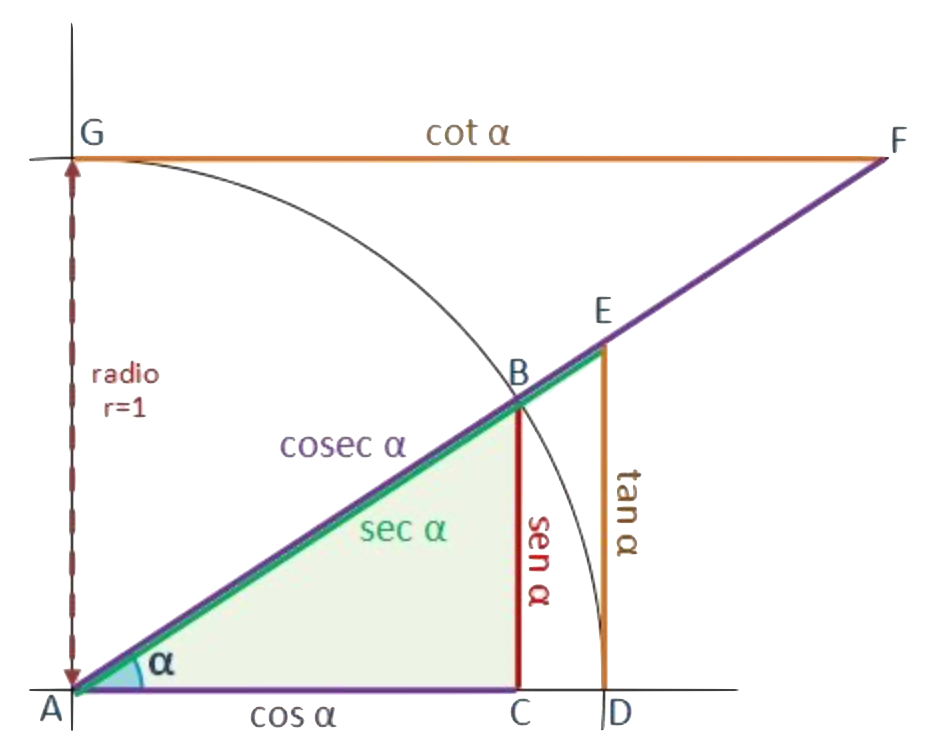
\includegraphics[width=0.45\textwidth]{img-rt/rt10.png}
\end{figure}
\end{multicols}	

Por ejemplo: Los triángulo $ABC \ \sim \ AED$ son semejantes, por ello,

\vspace{2mm} $\dfrac{BC}{AC}=\dfrac{ED}{AD} \ \to \ \dfrac{\sin \alpha}{\cos \alpha}=\dfrac{\tan \alpha}{1} \ \Rightarrow \ \ \tan \alpha\ = \ DE$

\vspace{2mm} Del mismo modo se pueden demostrar las restantes razones trigonométricas. \emph{Se deja como ejercicio}.
\end{myalertblock}

\begin{figure}[H]
	\centering
	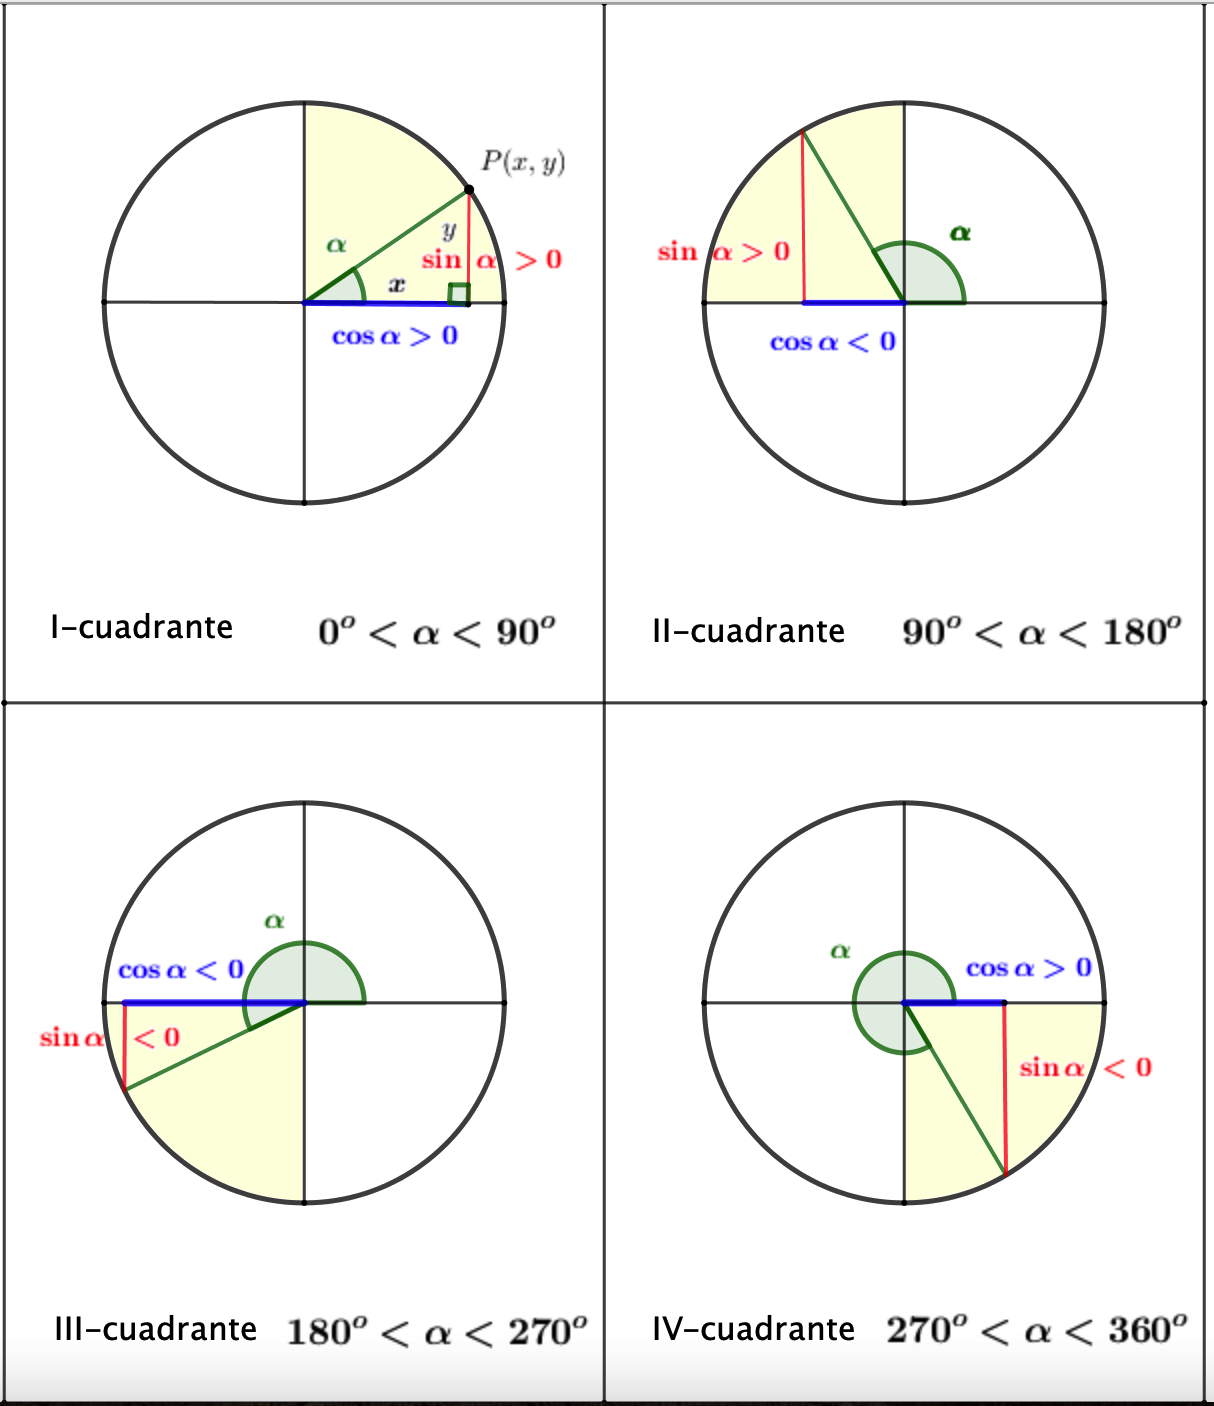
\includegraphics[width=0.9\textwidth]{img-rt/rt07.png}
\end{figure}







\subsection{Relación de ángulos de cualquier cuadrante con el primero}
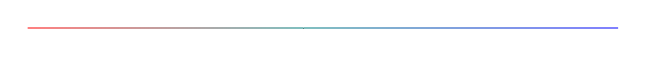
\begin{tikzpicture}
	\fill [left color=red!50, right color=teal!50] (0,0) rectangle (3.5,.01);
	\fill [left color=teal!50, right color=blue!50] (3.5,0) rectangle (7.5,.01);
	\end{tikzpicture}
\vspace{0.5cm}

\begin{large}\textbf{Relación de ángulos del  II-cuadrante con ángulos de I-cuadrante}\end{large}

\vspace{3mm}
\begin{theorem}[ Ángulos suplementarios]

Dos ángulos $\alpha$ y $\beta$	se dice que son \emph{\textbf{suplementarios}} si suman $\alpha+\beta=180^o = \pi $ rad.

\vspace{2mm} Dado un ángulo $\ \alpha\ $, su \emph{suplementario} será $\  \beta=180^o-\alpha$

\vspace{2mm}\textbf{Los ángulos suplementarios tienen los senos iguales}.
\end{theorem}



\vspace{0.2cm}
\begin{large}\textbf{Relación de ángulos del  III-cuadrante con ángulos de I-cuadrante}\end{large}

\vspace{2mm}
\begin{theorem}[ Ángulos que se diferencian en un llano]

Dos ángulos $\alpha$ y $\beta$	se dice que son \emph{\textbf{ángulos que se diferencian en un llano}} si su diferencia es  $\beta-\alpha=180^o = \pi $ rad.

\vspace{2mm} Dado un ángulo $\ \alpha\ $, su ángulo que \emph{se diferencia en 180$^o$} será $\beta=180^o+\alpha$

\vspace{2mm}\textbf{Los ángulos que se diferencian en $180^o$ tienen las tangentes iguales}.
\end{theorem}

\vspace{0.2cm}
\begin{large}\textbf{Relación de ángulos del  IV-cuadrante con ángulos de I-cuadrante}\end{large}

\vspace{2mm}
\begin{theorem}[ Ángulos opuestos]

Dos ángulos $\alpha$ y $\beta$	se dice que son \emph{\textbf{opuestos}} si suman $\beta+\alpha=360^o = 2\pi $ rad.

\vspace{2mm} Dado un ángulo $\ \alpha\ $, su \emph{opuesto} será $\ \beta= 360^o-\alpha$

\vspace{2mm}\textbf{Los ángulos opuestos tienen los cosenos iguales}.
\end{theorem}


\vspace{0.2cm}
\begin{large}\textbf{Relación de ángulos del  I-cuadrante con ángulos de I-cuadrante}\end{large}

\vspace{2mm}
\begin{theorem}[ Ángulos complementarios]

Dos ángulos $\alpha$ y $\beta$	se dice que son \emph{\textbf{complementarios}} si ente ambos completan un ángulo recto, si suman  $\beta+\alpha=90^o = \pi/2 $ rad. (o múltiplos de $\pi/2$ - ver ejemplo siguiente)

\vspace{2mm} Dado un ángulo $\ \alpha\ $, su \emph{complementario} será $\ \beta= 90^o-\alpha$

\vspace{2mm}\textbf{Los ángulos complementarios intercambian los papeles de seno y coseno}.
\end{theorem}

\begin{multicols}{2}
\begin{figure}[H]
	\centering
	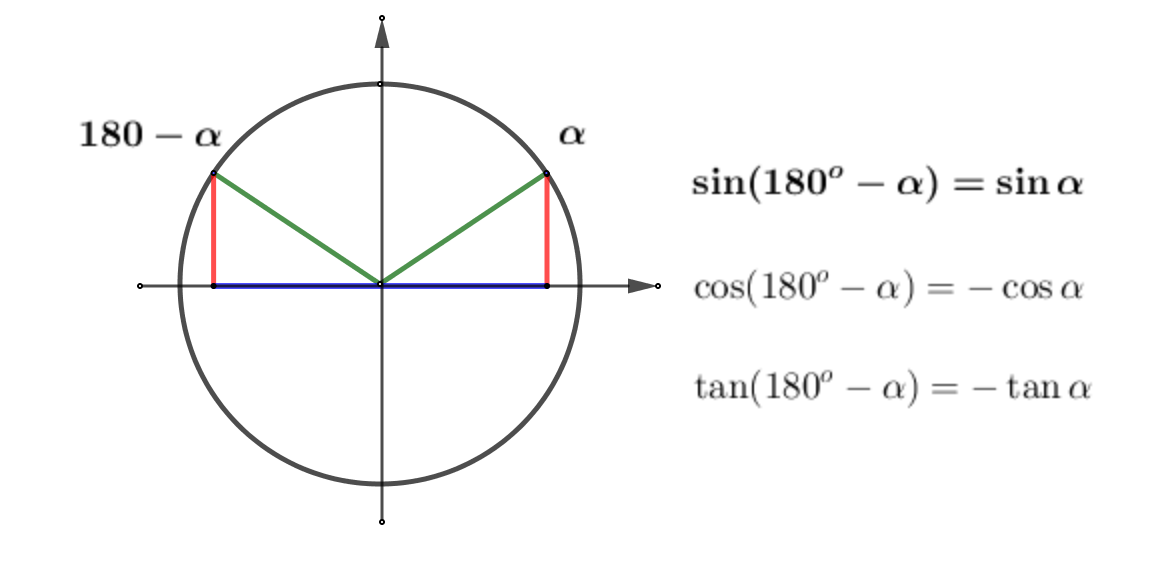
\includegraphics[width=0.45\textwidth]{img-rt/rt11.png}
	\caption*{\scriptsize{ángulos suplementarios}}
\end{figure}

\begin{figure}[H]
	\centering
	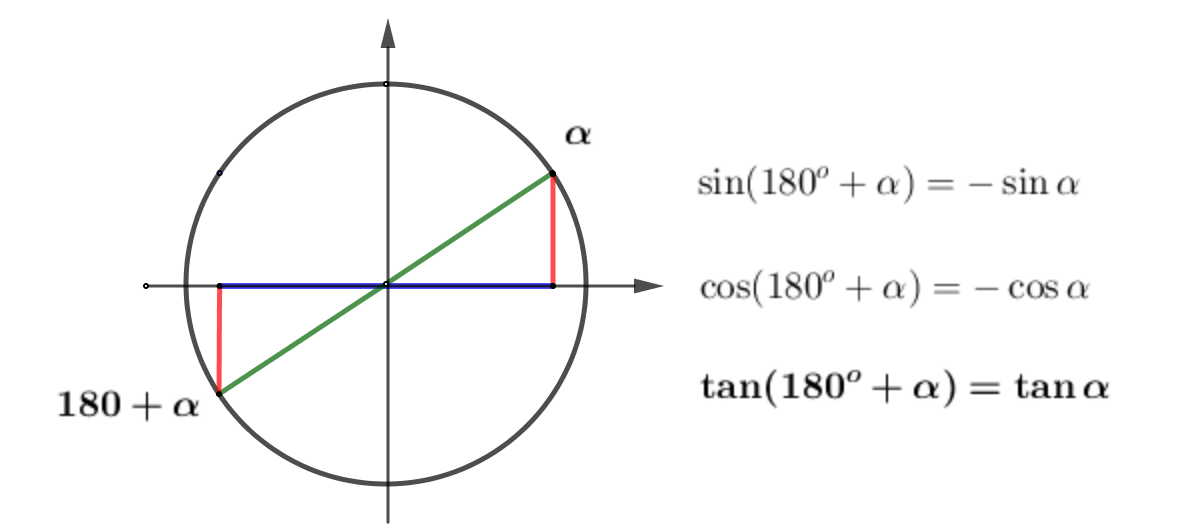
\includegraphics[width=0.45\textwidth]{img-rt/rt12.png}
	\caption*{\scriptsize{ángulos que se diferencian en 180$^o$}}
\end{figure}
\end{multicols}

\begin{multicols}{2}
\begin{figure}[H]
	\centering
	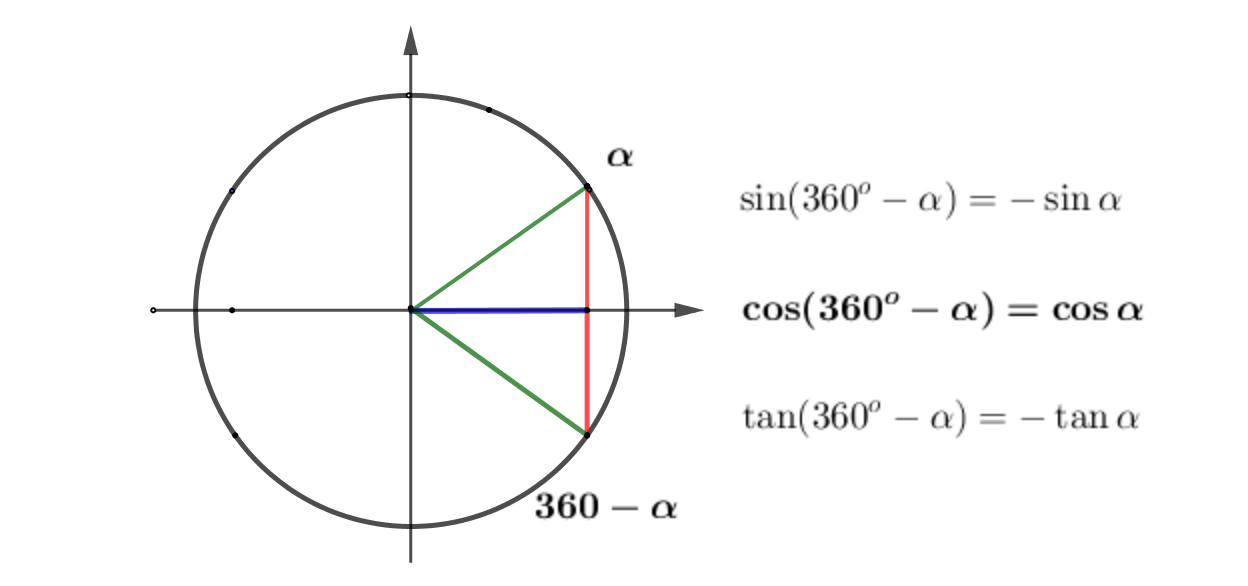
\includegraphics[width=0.45\textwidth]{img-rt/rt13.png}
	\caption*{\scriptsize{ángulos opuestos}}
\end{figure}

\begin{figure}[H]
	\centering
	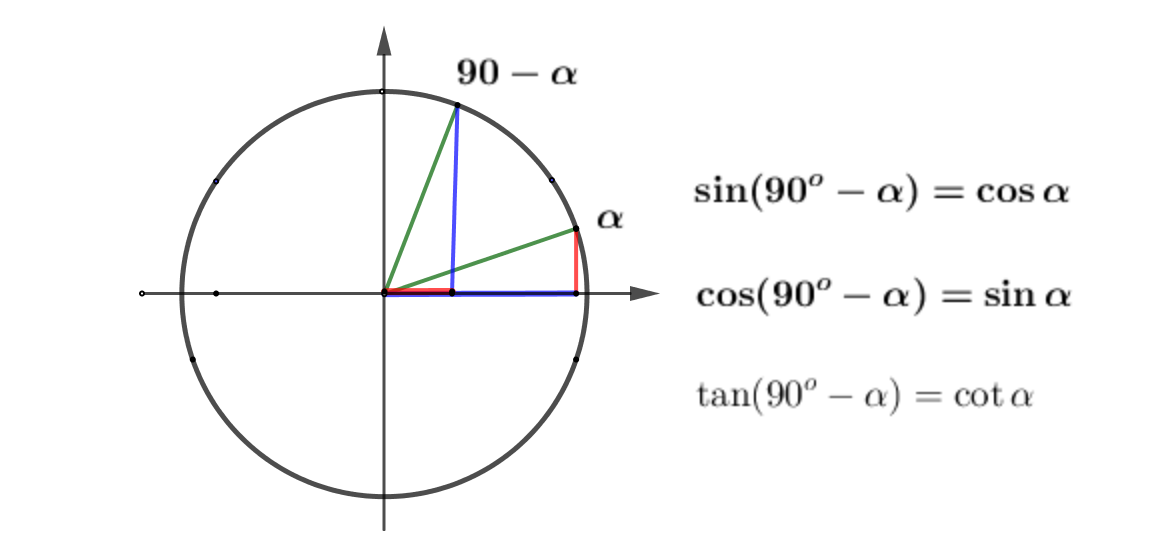
\includegraphics[width=0.45\textwidth]{img-rt/rt14.png}
	\caption*{\scriptsize{ángulos complementarios}}
\end{figure}
\end{multicols}

Todas estas relaciones no es necesario aprenderlas de memoria, sí entenderlas muy bien. En cada caso que se presente bastará con dibujar los ángulos correspondientes y razonar sobre el dibujo.
\vspace{5mm}
\begin{miejemplo}
	. Calcula las razones trigonométricas (RT) de los ángulos: 
	$\ 120^o;\quad 225^o;\quad 330^o; \quad 150^o,\ $ conocidas las RT de los ángulos notables.
	
\begin{footnotesize} \vspace{2mm}\textcolor{gris}{En adelante, cuando nos pregunten por las RT consideraremos solo el seno, coseno y tangente.} \end{footnotesize}
	
\begin{figure}[H]
	\centering
	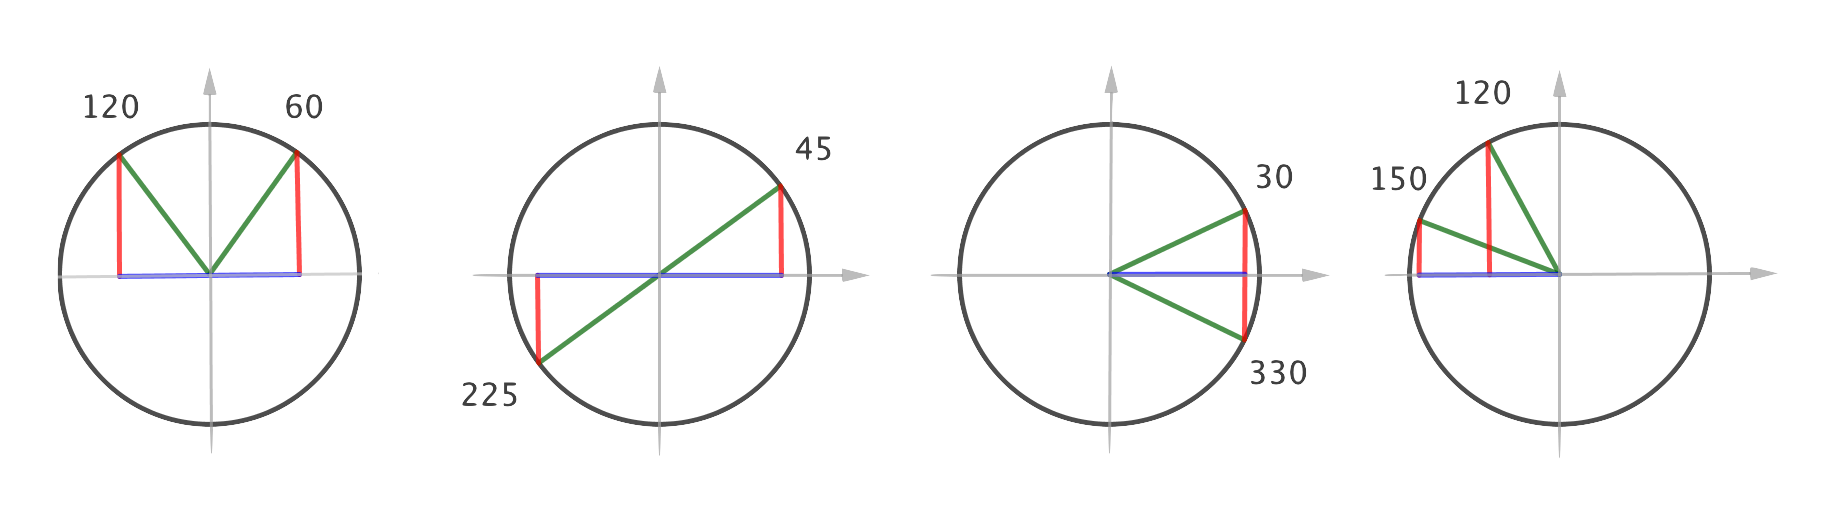
\includegraphics[width=0.95\textwidth]{img-rt/rt15.png}
\end{figure}

$\triangleright \quad  120^o \text{ y } 60^o$ tienen los mismos senos: 

$\sen 120=\sin 60=\dfrac{\sqrt{3}}{2};\ \ \cos 120=-\cos 60=-\dfrac 1 2; \ \ \tan 120= -\tan 60=-\sqrt{3}$

\vspace{4mm} $\triangleright \quad 225^o \text{ y } 45^o$ tienen las mismas tangentes:

$\sin 225=-\sin 45=-\dfrac{\sqrt{2}}{2};\ \ \cos 225=-\cos 45=-\dfrac{\sqrt{2}}{2};\ \ \tan 225=\tan 45=1$

\vspace{4mm} $\triangleright \quad 330^o \text{ y } 30^o$ tiene los mismos cosenos:

$\sin 330=-\sin 30=-\dfrac 1 2 ;\ \  \cos 330=\cos 30=\dfrac{\sqrt{3}}{2};\ \ \tan 330=-\tan 30 =-\dfrac{\sqrt{3}}{3}$

\vspace{4mm} $\triangleright \quad 120^o \text{ y }150^o$ intercambian los papeles de senos y coseno (salvo signos):

$\sin 150=-\cos 120=-(-\dfrac 1 2)=\dfrac 1 2;\ \ \cos 150=-\sin 120=-\dfrac{\sqrt{3}}{2};\ \ $

$\tan 150 = \dfrac{\sin 150}{\cos 150}=\dfrac{1/2}{-\sqrt{3}/2}= -\sqrt{3}/3$

\end{miejemplo}

\begin{miejemplo}

Calcula las razones trigonométricas de los ángulos de $25230^o$ y de $-103\pi/4$ rad.

\vspace{5mm} $\triangleright \quad 25230^o$ es un ángulo que `se pasa de vueltas' (mayor a $360^o$), dividiendo entre 360 averiguamos que se trata de una ángulo que ha dado $70$ vueltas (cociente) y $30^o$	 (resto). Si dibujamos el ángulo en la circunferencia goniométrica caerá exactamente encima del ángulo de $30^o$ (tras dar 70 vueltas -- no hacerlo-- \smiley{} )

\vspace{2mm} $\sin 25230=\sin 30=1/2;\quad \cos 25230=\cos 30=\sqrt{3}/3;\quad \tan 25230=\tan 30=\sqrt{3}/3$

\vspace{5mm} $\triangleright \quad -103\pi/4$ rad $\ = -\dfrac{103 \pi}{4} \dfrac{180}{\pi}=-9270^o$, ángulo que además de `pasado de vueltas' está medido al revés', en sentido negativo.

\vspace{2mm} Dividiendo el ángulo entre $360$, el cociente es $12$ y el resto $315$, pero se trata de un ángulo negativo así que se dan 12 vueltas al revés (en sentido de las agujas del reloj) y 315 grados en sentido negativo.  Luego $-9270^o = -12 \text{ vueltas y } -315^o$, las razones trigonométricas de $-9270^o$ serán las mismas que las de $-315^o$

\vspace{2mm} Si a un ángulo se le suma una vuelta completa, el ángulo queda en la circunferencia goniométrica en la misma posición, tendrán las mismas razones trigonométricas: $-315^0 \equiv -315+360=45^o$, así $\quad \sin(-103\pi/4)=\sin 45=\sqrt{2}/2;\quad \cos(-103\pi/4)=\cos 45=\sqrt{2}/2;\quad \tan(-103\pi/4)=\tan 45=1$


\end{miejemplo}


\begin{miejercicio}
. Si 	$\sin \alpha=3/5$ y $\alpha \in I-\text{cuadrante}\, , \ $ ?`cuáles son las restantes RT de $\alpha$?

\rule{250pt}{0.1pt}	

\vspace{5mm} Acudiendo a la relación fundamental de la trigonometría,

\vspace{2mm}  $\sin^2 \alpha + \cos^2 \alpha = 1 \ \to \ (3/5)^2 + \cos^2 \alpha = 1 \ \to \ \cos^2 \alpha = 1-(3/5)^2=1-9/25=16/25$

\vspace{2mm} Para calcular $\cos \alpha$ a partir de $\cos^2 \alpha$ tenemos la doble posibilidad de signo, $|\cos \alpha|=\sqrt{16/25}=4/5 \ \to \ \cos \alpha=\pm 4/5$, como estamos en el primer cuadrante y allí los cosenos son positivos, elegimos:
$\ \boldsymbol{\cos \alpha =4/5} \ \to \ \boldsymbol{\tan \alpha}=\sin \alpha / \cos \alpha = (3/5)/(4/5)=\boldsymbol{3/4}$
\end{miejercicio}


\begin{miejercicio}
. Sabiendo que $\tan \alpha=-2$ y que $90^o<\alpha <180^o$ \textcolor{gris}{(segundo cuadrante)}, calcula las restantes razones trigonométricas. 

\rule{250pt}{0.1pt}	


\vspace{5mm} \begin{multicols}{2}
De una de las relaciones derivadas de la relación fundamental de la trigonometría, tenemos que:
$\tan^2 \alpha + 1 = \sec^2 \alpha \ \to \ $

\vspace{2mm} $\to \sec^2 \alpha=(-2)^2+1=5=\dfrac{1}{\cos ^2 \alpha}$

\vspace{2mm} Doble posibilidad de signo: 

\vspace{2mm} $\cos \alpha=\pm \dfrac 1 {\sqrt{5}}=\pm \dfrac{\sqrt{5}}{5}$

\vspace{2mm} $\alpha \in II \text{ cuadrante } \Rightarrow \ \cos \alpha < 0$
 \begin{figure}[H]
	\centering
	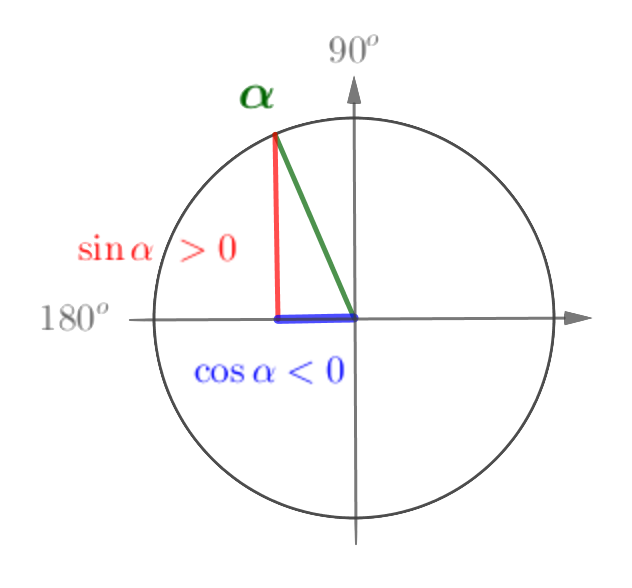
\includegraphics[width=0.4\textwidth]{img-rt/rt16.png}
\end{figure}
\end{multicols}
Luego: $\ \boldsymbol{\cos \alpha}=	- \dfrac {1}{\sqrt{5}}= \boldsymbol{-\dfrac{\sqrt{5}}{5}} \quad \to \ \boldsymbol{\sin \alpha} =\tan \alpha \cdot \cos \alpha = -2\, \left( - \dfrac{\sqrt{5}}{5}  \right) = \boldsymbol{\dfrac{2\sqrt{5}}{5}}$
\end{miejercicio}



\begin{miejercicio}

Sabiendo que $\ \cot \alpha=-3\ $ y que $270<\alpha<360$, encuentra $\sin \alpha$ y $\cos \alpha$

\vspace{2mm} Mediante un dibujo adecuado en cada caso, a partir de las RT de $\alpha$, calcula:

\vspace{2mm} $\sin(90+\alpha);\ \ \cos(90-\alpha);\ \ \tan(180-\alpha);\ \ \sec(180+\alpha);\ \ \tan(360-\alpha);\ \ \csc(360+\alpha)$ 

\rule{250pt}{0.1pt}	

\vspace{2mm} $\cot \alpha=-3 \ \to \ \tan=-1/3 \ \Rightarrow \ \tan^2 \alpha+1=\sec^2=\dfrac{1}{\cos^2 \alpha} \ \to \  \cos \alpha=\pm \dfrac{3\sqrt{10}}{10}$

\vspace{2mm} \begin{footnotesize} \textcolor{gris}{También hubiésemos podido acudir a $\cot^2 \alpha+1=\csc^2 \alpha$, pero lo hacemos así por no recordar demasiadas fórmulas (de momento \frownie{}, en el tema posterior aparecerán muchas más)} \end{footnotesize}

\vspace{2mm} Como por hipótesis estamos en el IV cuadrante, el coseno es positivo,

$\boldsymbol{\cos \alpha= \dfrac{3\sqrt{10}}{10}} \quad \to \quad \boldsymbol{\sin \alpha}= \tan \alpha \cdot \cos \alpha =\boldsymbol{-\dfrac{\sqrt{10}}{10}}$

\vspace{2mm}
Para dibujar los ángulos, p.e. $90+\alpha$, nos situamos en $90^o$ (OY positivo) y, desde allí, medimos  $\alpha$ (3 rectos y un ángulo agudo más, estamos en el tercer cuadrante), en las figuras hemos elegido éste como de unos $60^o$, resultando $\alpha$ un ángulo de unos $330^o$. Para dibujar $90-\alpha$, a partir de $90$ medimos $\alpha$ (tres rectos y $60^0$) en sentido negativo. También podemos imaginar que $\alpha=330^o$ y $90-\alpha=90-330=-240=-240+360=120$, en el segundo cuadrante.

\vspace{-6mm}
\begin{center} \rule{300pt}{0.1pt} \end{center}

\begin{multicols}{2}
Seno nuevo ángulo igual a coseno del antiguo, ambos $(+)$ (el coseno de 90+$\alpha$ $(+)$ es opuesto al seno de $\alpha$ $(-)$)

$\quad$

$\qquad \sin (90+\alpha)=\cos \alpha=\dfrac{3\sqrt{10}}{10}$
\begin{figure}[H]
	\centering
	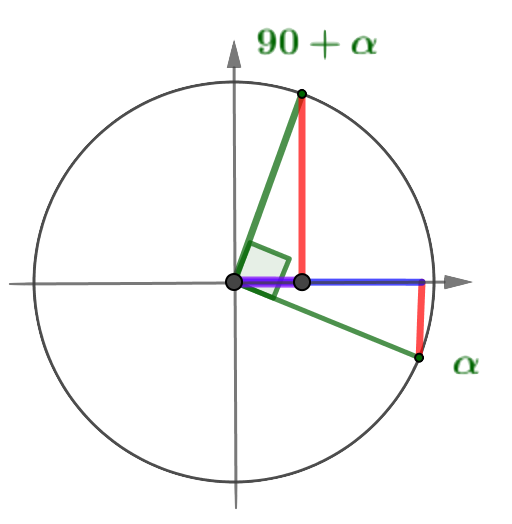
\includegraphics[width=0.23\textwidth]{img-rt/rt17.png}
	\end{figure}	
\end{multicols}
\vspace{-6mm}
\begin{center} 
\vspace{-5mm}
\rule{300pt}{0.1pt} \end{center}

\begin{multicols}{2}
\begin{figure}[H]
	\centering
	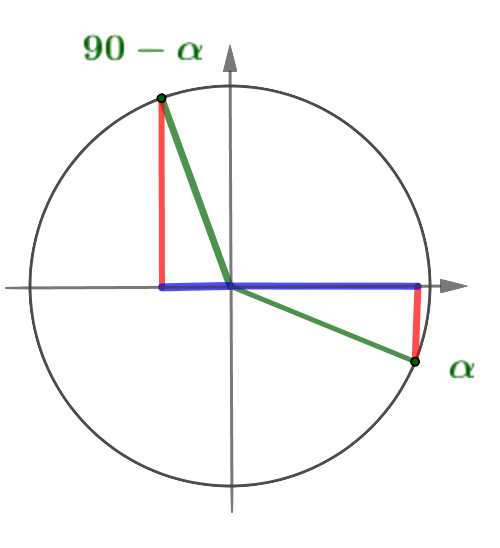
\includegraphics[width=0.23\textwidth]{img-rt/rt18.png}
	\end{figure}	
Intercambio senos por coseno.

$\quad$

$\qquad \cos(90-\alpha)=\sin\alpha=-\dfrac{\sqrt{10}}{10}$
\end{multicols}

\begin{center} 
\vspace{-6mm}
\rule{300pt}{0.1pt} \end{center}

\begin{multicols}{2}
Senos iguales, cosenos opuestos.

$\quad$

$\qquad \tan (180-\alpha)=\dfrac{\sin(180-\alpha)}{\cos(180-\alpha)}$


$\qquad =\dfrac{\sin \alpha}{-\cos \alpha}= \dfrac{-\sqrt{10}/10}{-3\sqrt{10}{10}}=\dfrac 1 3$
	\begin{figure}[H]
	\centering
	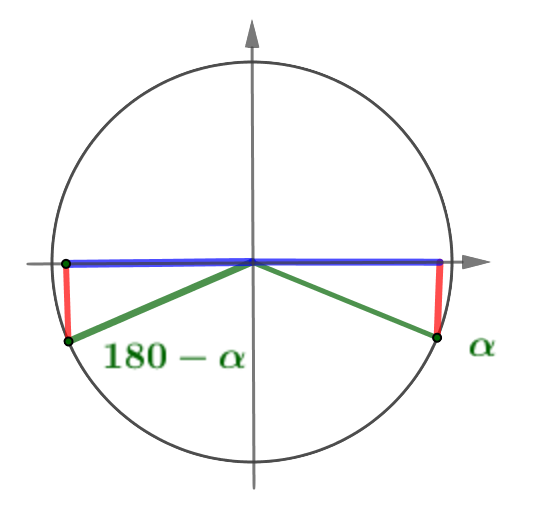
\includegraphics[width=0.25\textwidth]{img-rt/rt19.png}
	\end{figure}
\end{multicols}

\begin{center} 
\vspace{-6mm}
\rule{300pt}{0.1pt} \end{center}

\begin{multicols}{2}

\begin{figure}[H]
	\centering
	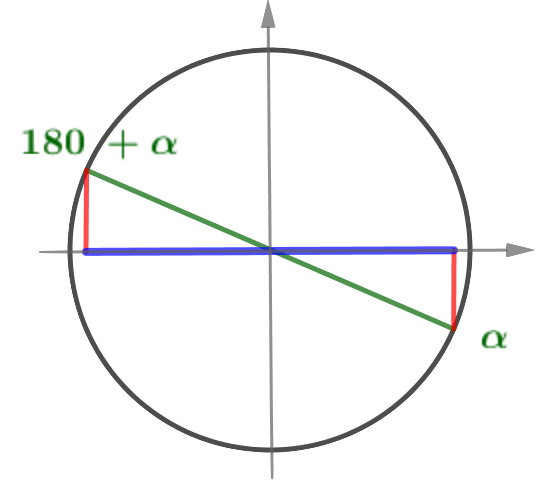
\includegraphics[width=0.25\textwidth]{img-rt/rt20.png}
	\end{figure}
Tangentes iguales.
	
$\quad$
	
$\qquad \sec(180+\alpha)=\dfrac{1}{\cos(180+\alpha)}=$

$\qquad \dfrac{1}{-\cos \alpha}=\dfrac{1}{-3\sqrt{10}/10}=-\dfrac{\sqrt{10}}{3}$
		
\end{multicols}

\begin{center} 
\vspace{-6mm}
\rule{300pt}{0.1pt} \end{center}

\begin{multicols}{2}
Cosenos iguales.

$\quad$

$\qquad \tan (360-\alpha)=\dfrac{\sin (360-\alpha)}{\cos (360-\alpha)}=$

$\qquad =\dfrac{\cos \alpha}{-\sin \alpha}=-\tan \alpha = \dfrac 1 3 $

\begin{figure}[H]
	\centering
	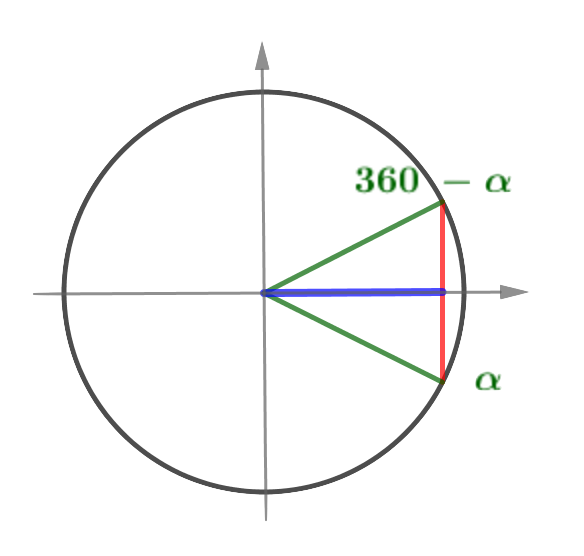
\includegraphics[width=0.25\textwidth]{img-rt/rt21.png}
	\end{figure}

		
\end{multicols}

\begin{center} 
\vspace{-6mm}
\rule{300pt}{0.1pt} \end{center}

\begin{multicols}{2}

\begin{figure}[H]
	\centering
	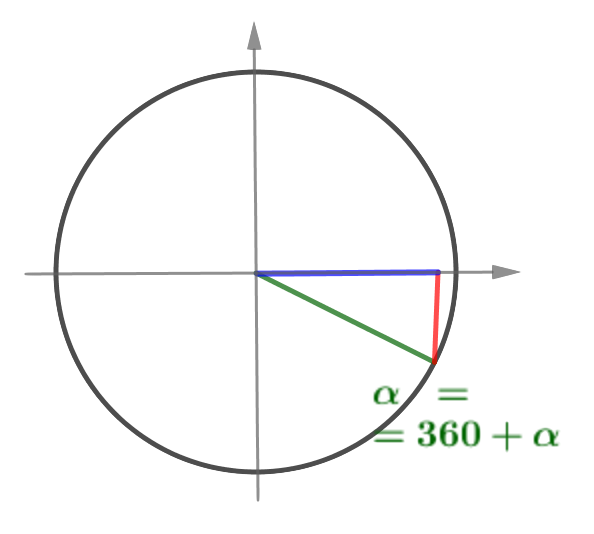
\includegraphics[width=0.25\textwidth]{img-rt/rt22.png}
	\end{figure}
Mismo ángulo.

$\quad$

$\qquad \csc (360+\alpha)=\dfrac{1}{\sin (360+\alpha)}=$

$\qquad =\dfrac {1}{\sin \alpha } = \dfrac {1}{-\sqrt{10}/10}=-\sqrt{10}$
		
\end{multicols}

\end{miejercicio}

\vspace{3mm}

\begin{small} \underline{Observación}: Podemos resolver todos los ejercicios anteriores sin necesidad de acudir a la relación fundamental de la trigonometría ni a sus derivadas, tan solo con el teorema de Pitágoras (que es de donde provienen). En cada caso, y prescindiendo de signos, dada una RT podemos dibujar un triángulo rectángulo cualquiera que la cumpla y encontrar el lado que falte; luego, según el cuadrante en que se esté, se eligen los signos a las RT encontradas.\end{small}

\begin{figure}[H]
	\centering
	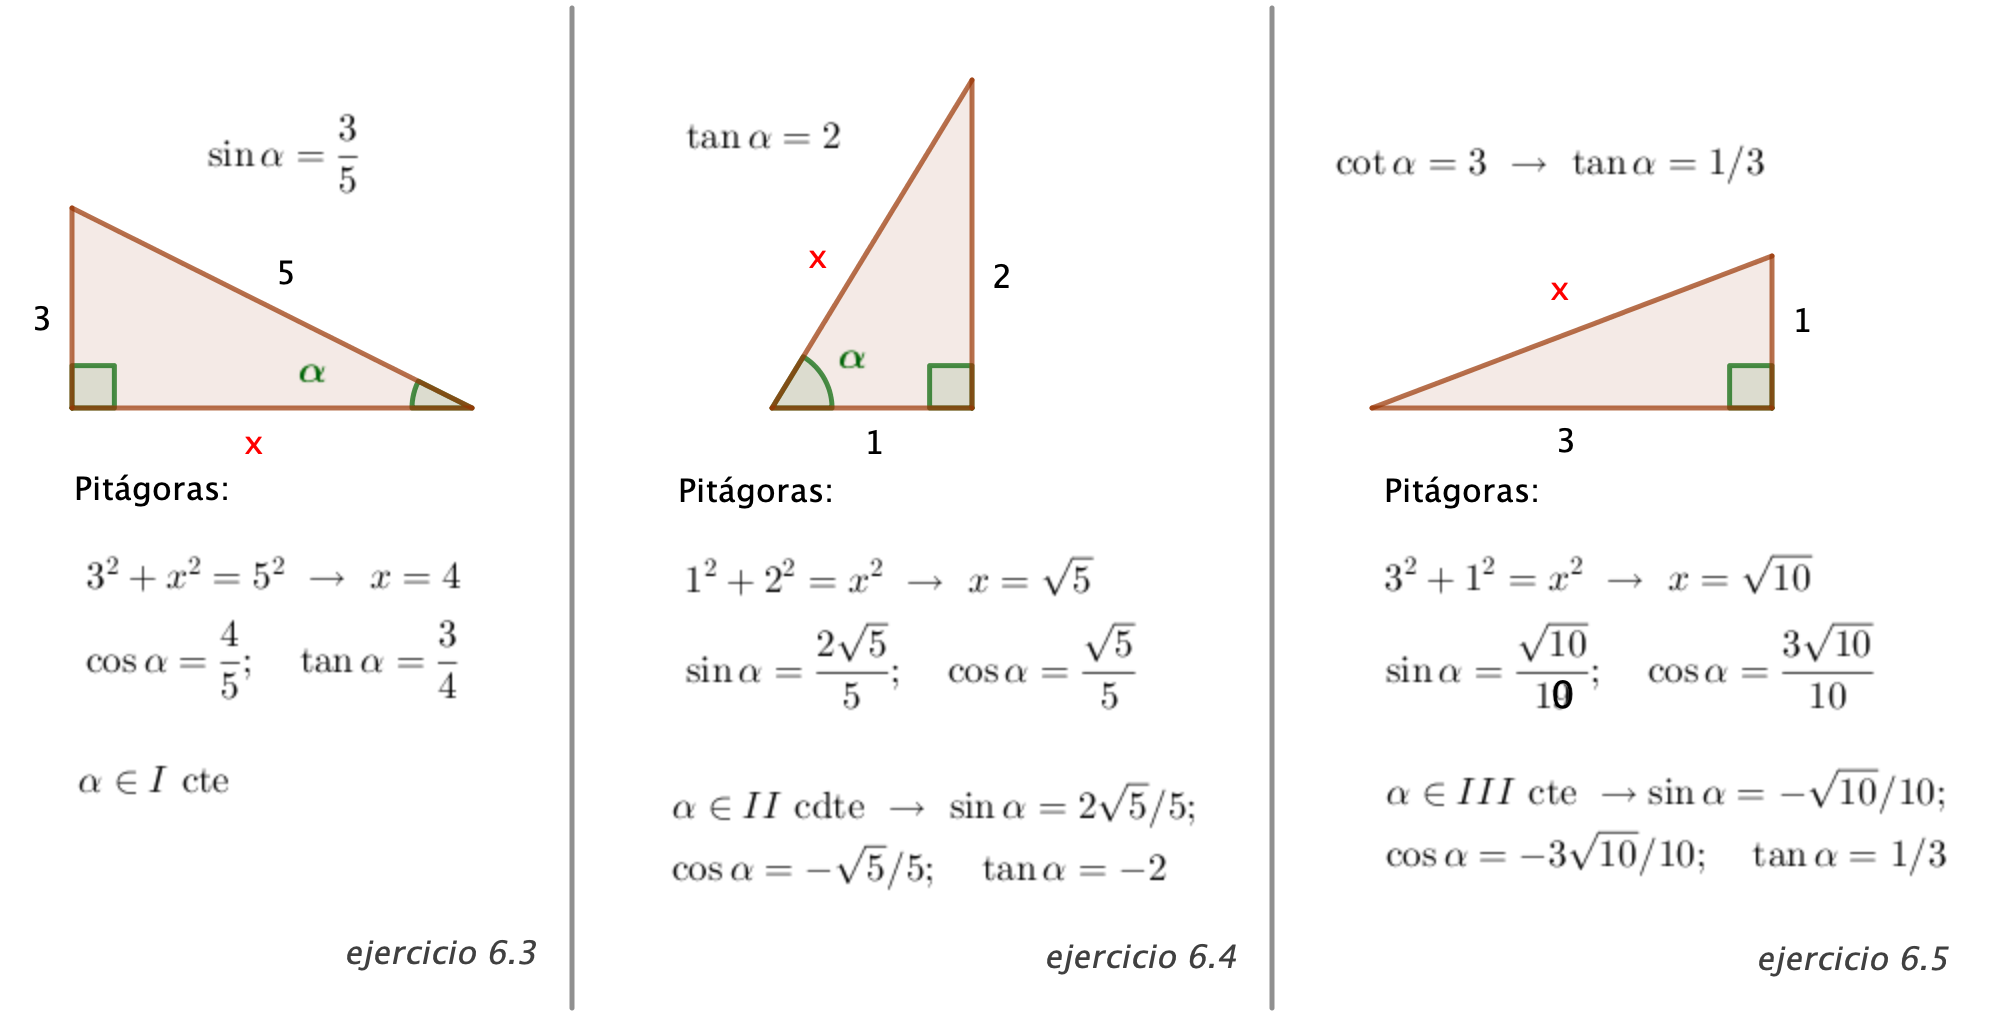
\includegraphics[width=1\textwidth]{img-rt/rt23.png}
\end{figure}

\subsection{Razones trigonométricas de los ángulos frontera entre cuadrantes}
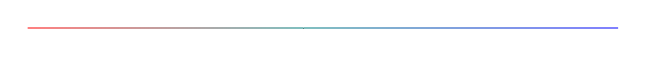
\begin{tikzpicture}
	\fill [left color=red!50, right color=teal!50] (0,0) rectangle (3.5,.01);
	\fill [left color=teal!50, right color=blue!50] (3.5,0) rectangle (7.5,.01);
	\end{tikzpicture}
\vspace{0.5cm}


\begin{multicols}{2}

Son ángulos frontera $0^o\equiv 360^o;\ 90^o;\ 180^o \text{ y } 270^o$.

Sus RT las veremos como un paso al límite.

P.e., el seno de $0^o$: a medida que nos acercamos a él, los senos (en rojo) son cada vez más pequeños y los cosenos (en azul) cada vez mayores, por lo que diremos que:

$$\sin 0=0;\qquad \cos 0=1$$

De forma análoga encontramos las restantes RT de los ángulos frontera.
\begin{figure}[H]
	\centering
	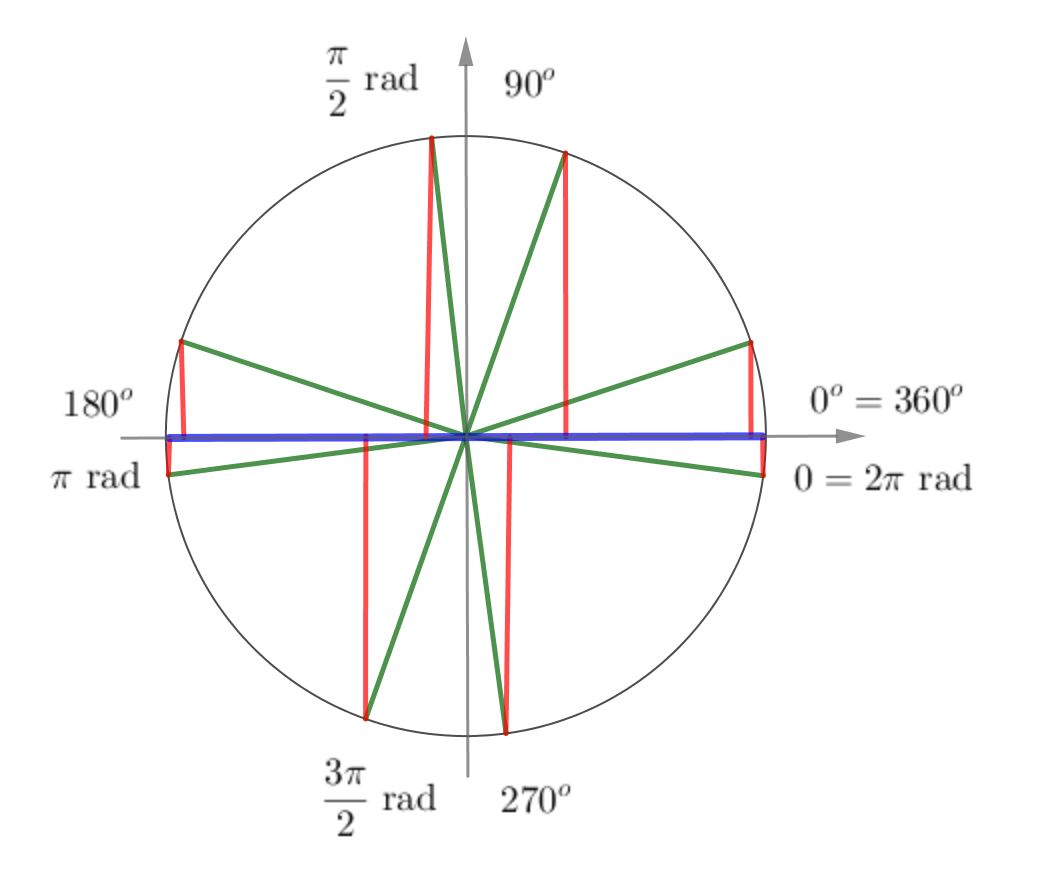
\includegraphics[width=.5\textwidth]{img-rt/rt25.png}
\end{figure}	
\end{multicols}

\begin{table}[H]
\centering
\begin{tabular}{|c|c|c|c|c|}
\hline
$\theta \ \ (^o)$ & $\quad 0 \quad$ & $\quad 90 \quad$ & $\quad 180 \quad$ & $\quad 270 \quad $ \\ \hline
$\theta \ $ (rad) & $0$ & $\pi/2$ & $\pi$ & $3\pi/2$ \\ \hline $-----$&$-----$&$-----$&$-----$&  $-----$ \\ \hline
$\sin \theta$ & $0$ & $1$ & $0$ & $-1$ \\ \hline
$\cos \theta$ & $1$ & $0$ & $-1$ & $0$ \\ \hline
$\tan \theta$ & $0$ & $\nexists$ & $0$ & $\nexists$ \\ \hline
\end{tabular}
\end{table}






\vspace{.5cm}
\section{Identidades trigonométricas I/II}

\begin{tikzpicture}
	\fill [left color=red!50, right color=teal!50] (0,0) rectangle (3.5,.1);
	\fill [left color=teal!50, right color=blue!50] (3.5,0) rectangle (7.5,.1);
	\end{tikzpicture} \hspace{1cm} \footnote{$\ $ Se ampliará en próximos temas}
\vspace{0.5cm}

Las identidades trigonométricas nos ayudan a simplificar expresiones complejas y de esta forma a comprender mejor el significado de la expresión.

Verificar una identidad trigonométrica consiste en demostrar que efectivamente ambos lados de la igualdad son equivalentes. Usaremos operaciones algebraicas e identidades trigonométricas conocidas para convertir uno de los lados de la ecuación exactamente en la forma en que está expresado el otro lado de la ecuación.
\vspace{5mm}
\begin{miejercicio}
. Demuestra las siguientes identidades trigonométricas.

\vspace{2mm} $a)\ \ \csc^2 \alpha-\cot^2\alpha=1 ; \qquad  \qquad \qquad  \qquad \quad b) \ \   \sin^2 \alpha-\cos^2 \beta=\sin^2 \beta - \cos^2 \alpha$

\vspace{2mm} $c)\ \ \sec^2 \alpha + \csc^2 \alpha=\sec^2 \alpha \cdot \csc^2 \alpha;\qquad  \qquad d)\ \ \dfrac{\cos \alpha}{1-\sin \alpha}-\dfrac{1+\sin \alpha}{\cos \alpha}=0$

\rule{250pt}{0.1pt}	

\vspace{5mm} $\triangleright \ \  a)\quad \csc^2 \alpha - \cot^2 \alpha = \dfrac{1}{\sin^2 \alpha}-\dfrac{1}{\tan^2 \alpha}=\dfrac{1}{\sin^2 \alpha}-\dfrac{\cos^2 \alpha }{\sin^2 \alpha}=\dfrac{1-\cos^2\alpha}{\sin^2 \alpha}=\dfrac{\sin^2 \alpha}{\sin^2 \alpha}=1$


\vspace{5mm} $\triangleright \ \  b)\quad \sin^2 \alpha-\cos^2 \beta= 1-\cos^2 \alpha-(1-\sin^2 \beta)=\cancel{1} -\cos^2 \beta -\cancel{1}+\sin^2 \beta=\sin^2 \beta - \cos^2 \alpha $


\vspace{5mm} $\triangleright \ \  c)\quad \sec^2 \alpha + \csc^2 \alpha= \dfrac{1}{\cos^2 \alpha} + \dfrac{1}{\sin^2 \alpha}= \dfrac{\sin^2 \alpha + \cos^2 \alpha}{\cos^2 \alpha \, \sin^2 \alpha}= \dfrac{1}{\cos^2 \alpha \, \sin^2 \alpha}=\dfrac{1}{\cos^2 \alpha}\, \dfrac
{1}{\sin^2 \alpha}=$

\vspace{2mm}\hspace{1.2cm} $\ = \sec^2 \alpha \cdot \csc^2 \alpha$

\vspace{5mm} $\triangleright \ \  d)\quad \dfrac{\cos \alpha}{1-\sin \alpha}-\dfrac{1+\sin \alpha}{\cos \alpha}=\dfrac{\cos^2 \alpha - (1-\sin^2 \alpha)}{\cos \alpha(1-\sin \alpha)}= \dfrac{\cos^2 \alpha - \cos^2 \alpha }{\cos \alpha(1-\sin \alpha)}=\dfrac{0}{\cos \alpha(1-\sin \alpha)}=0$

\end{miejercicio}








%********************************************************************
\vspace{1cm}
\section{Funciones trigonométricas}

\begin{tikzpicture}
	\fill [left color=red!50, right color=teal!50] (0,0) rectangle (3.5,.1);
	\fill [left color=teal!50, right color=blue!50] (3.5,0) rectangle (7.5,.1);
	\end{tikzpicture}
\vspace{0.5cm}

\begin{figure}[H]
	\centering
	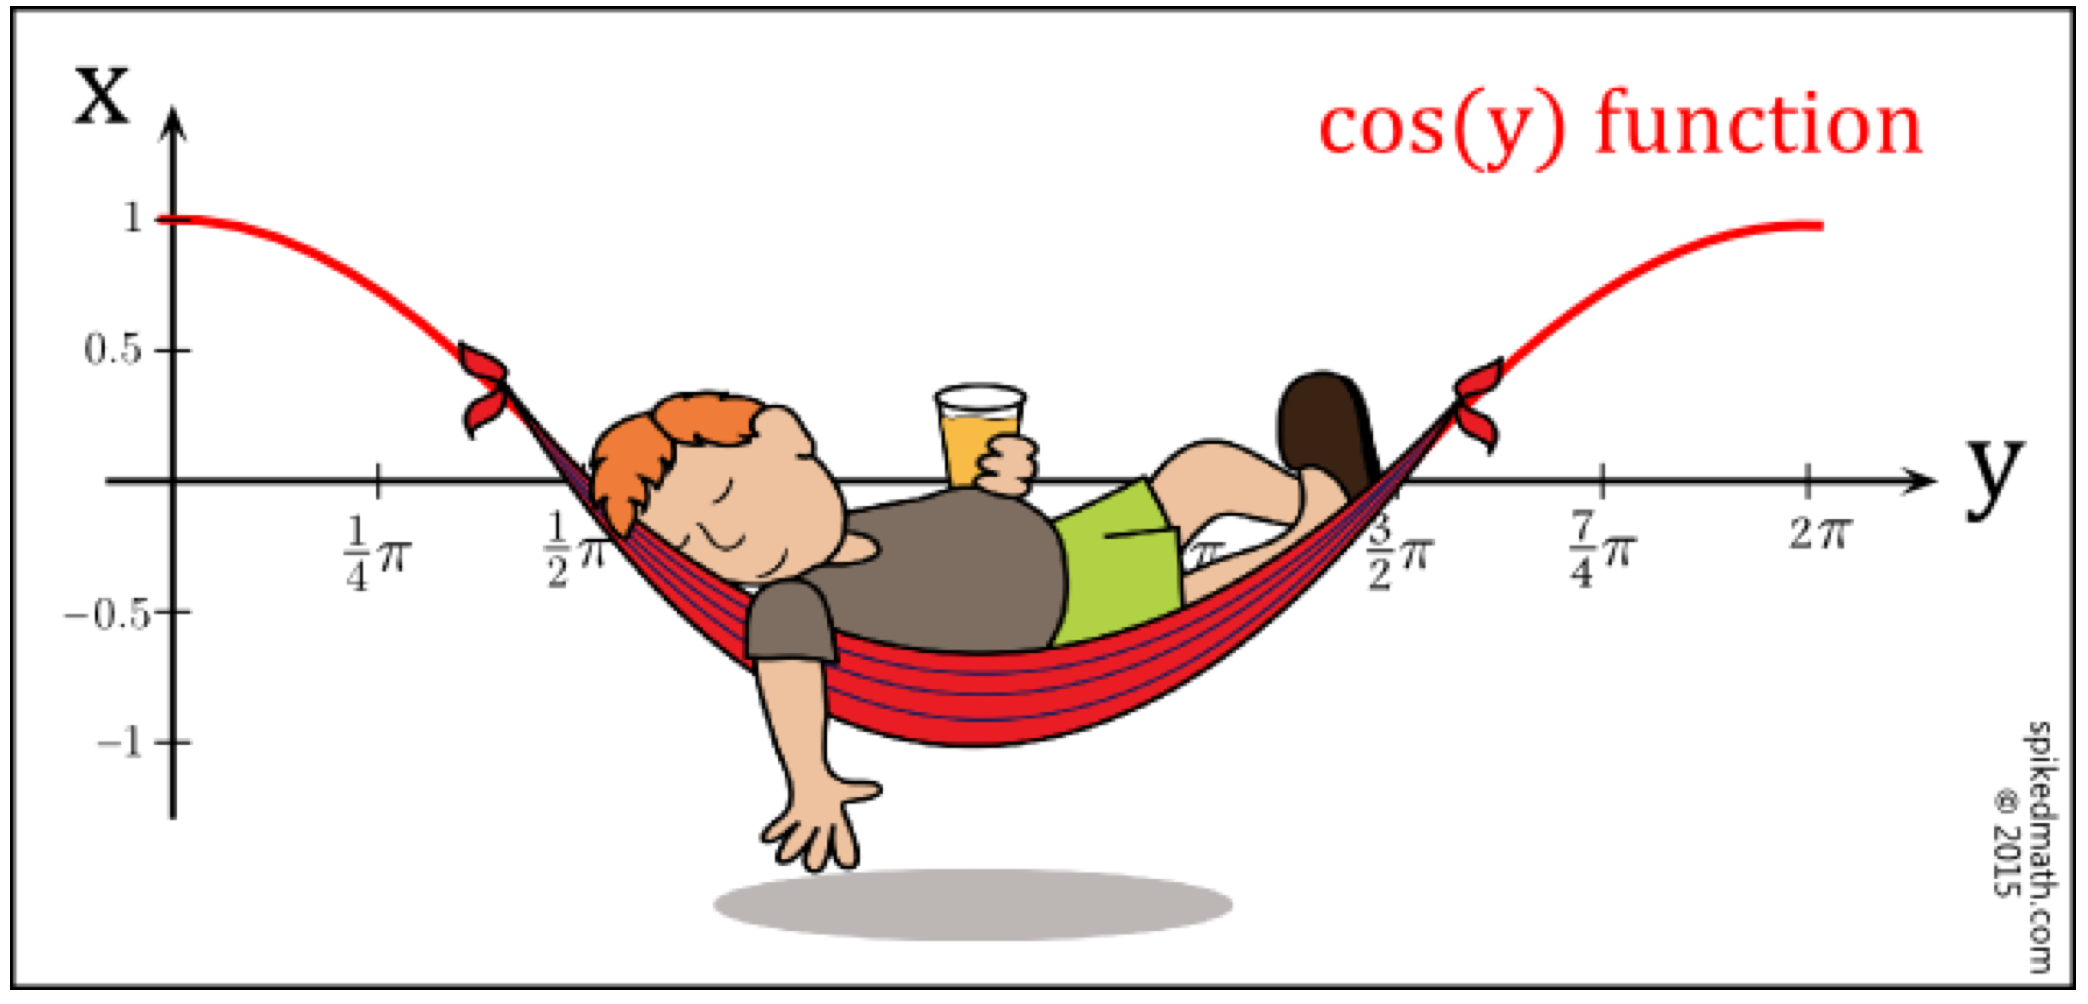
\includegraphics[width=0.6\textwidth]{img-rt/rt47.png}
\end{figure}


\begin{multicols}{2}
Aunque los conceptos que aquí veamos serán desarrollados con mayor profundidad en la parte de \emph{`Cálculo'}, esbozaremos la forma de las funciones trigonométricas seno, coseno y tangente.

Representando en unos ejes cartesianos los valores que toman seno, coseno y tangente, se obtienen las gráficas que aparecen en la siguiente figura.

Se aconseja hacerse una tabla con los valores de estas RT para los ángulos frontera y para los ángulos notables en todos los cuadrantes. 

\begin{figure}[H]
	\centering
	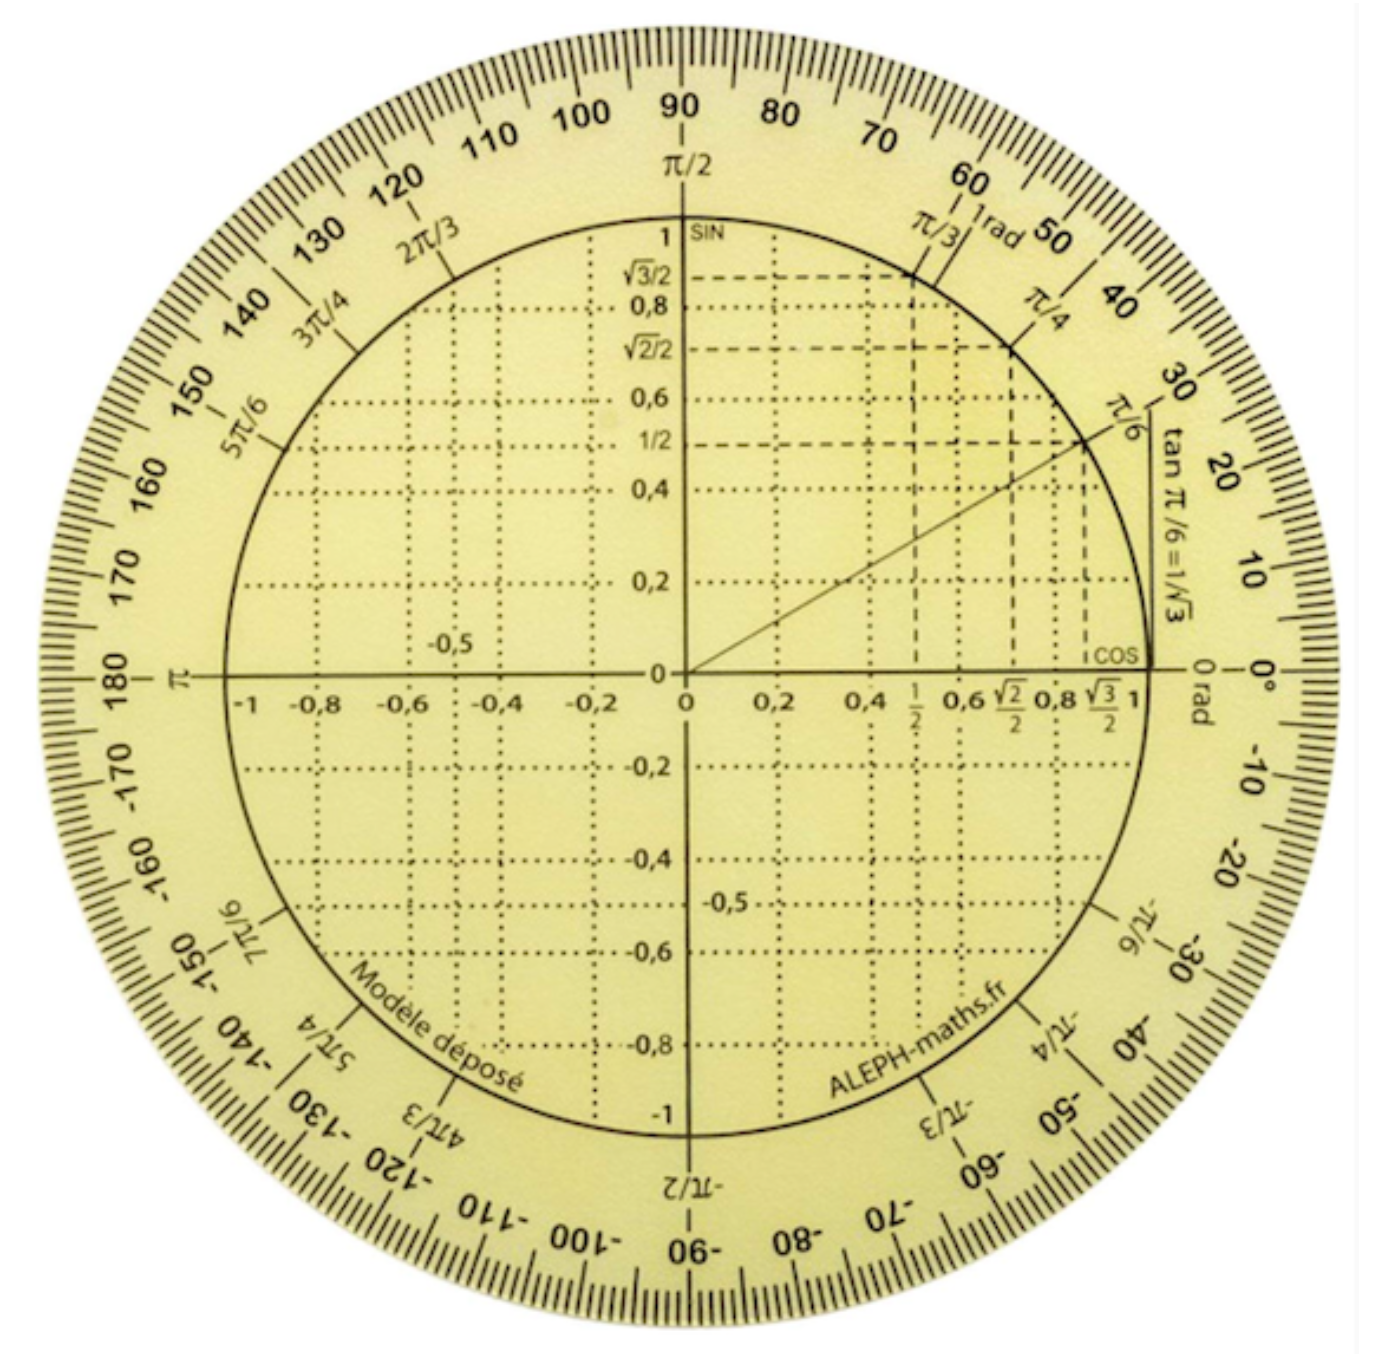
\includegraphics[width=.45\textwidth]{img-rt/rt26.png}
\end{figure}
\end{multicols}

\begin{figure}[H]
	\centering
	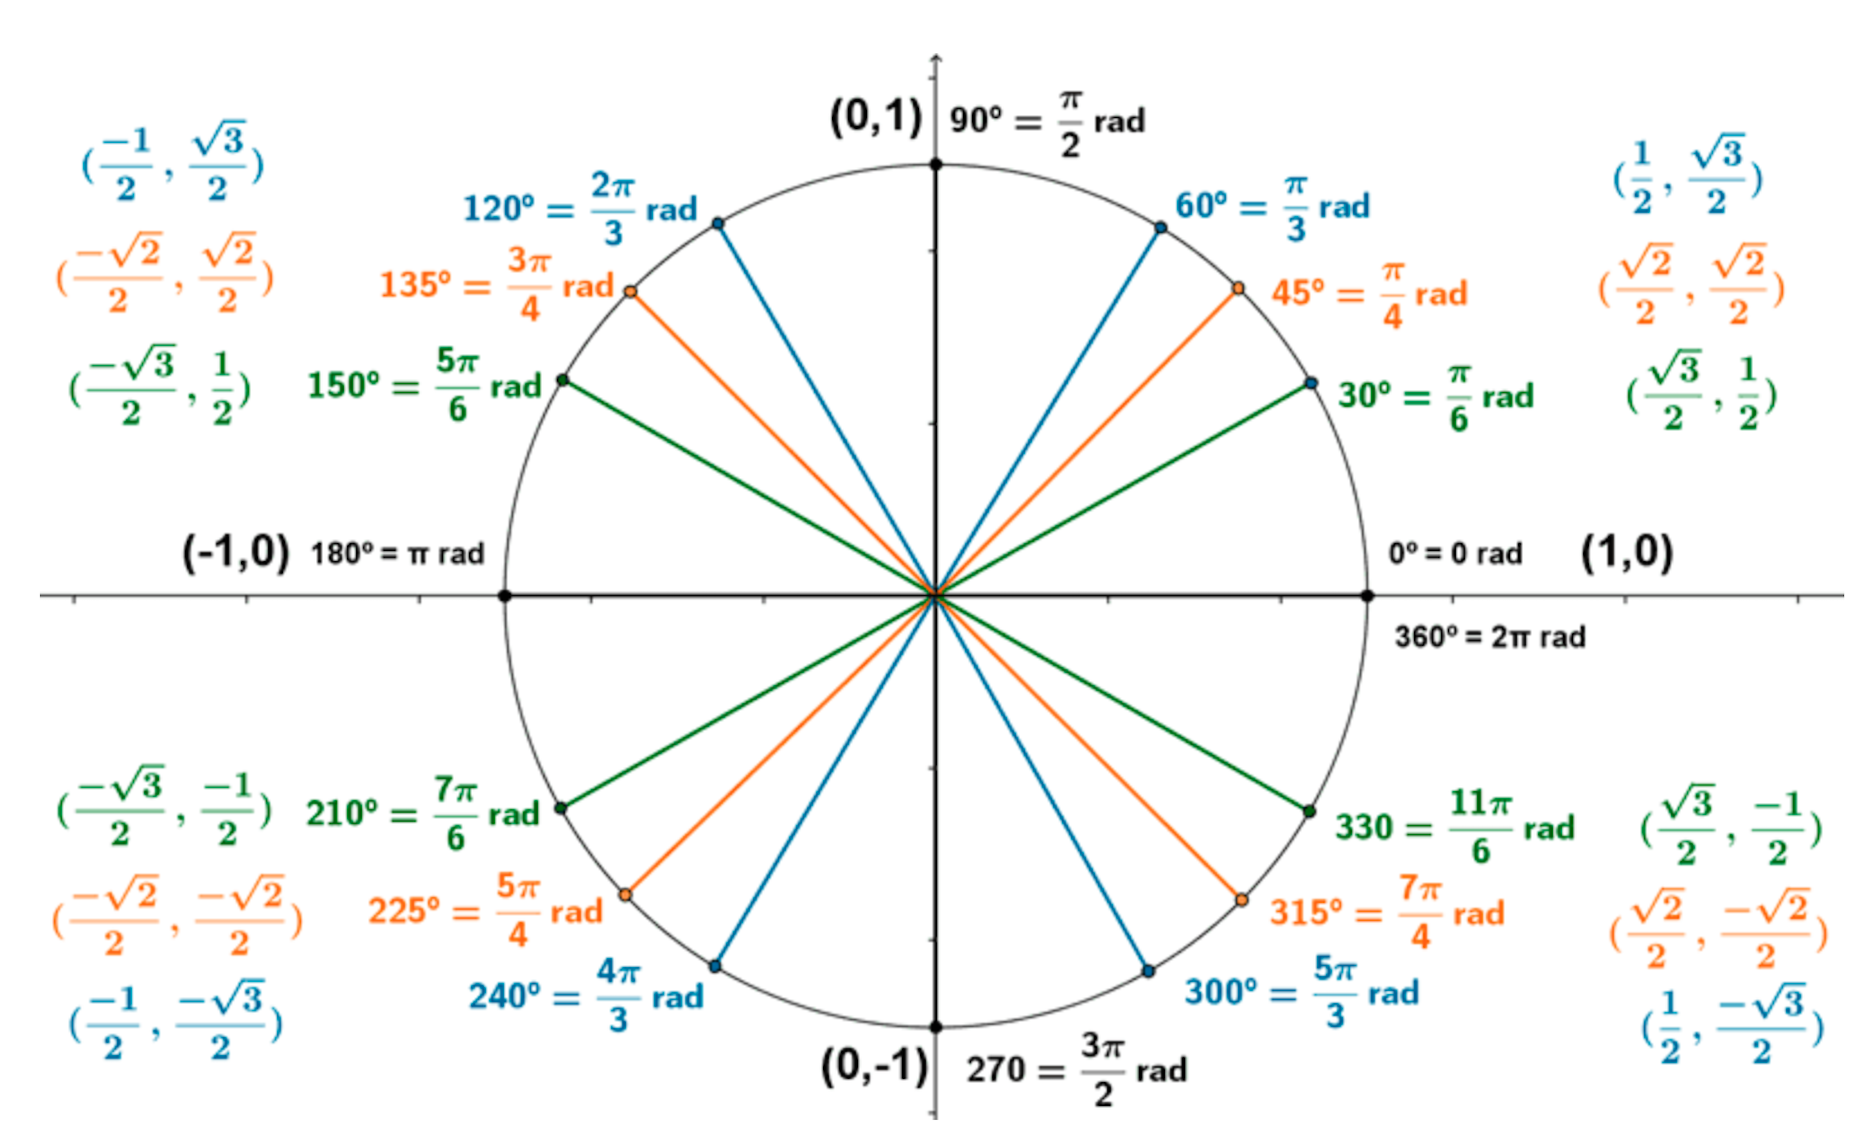
\includegraphics[width=.9\textwidth]{img-rt/rt50.png}
\end{figure}

\vspace{5mm}
\begin{figure}[H]
	\centering
	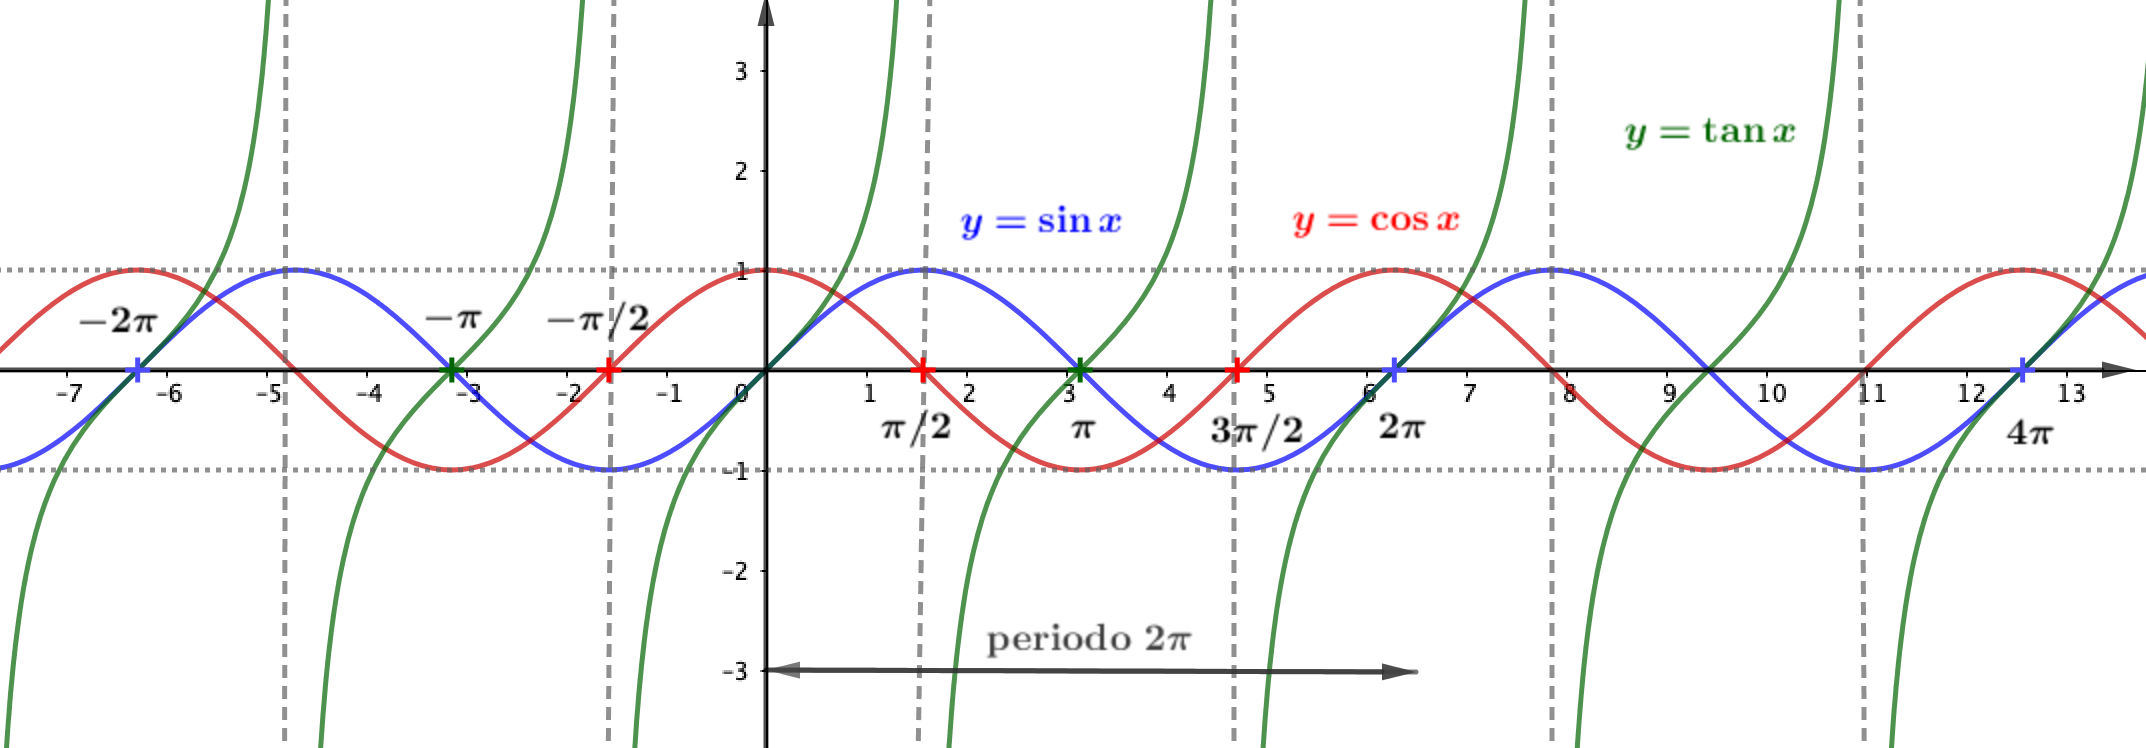
\includegraphics[width=1\textwidth]{img-rt/rt27.png}
\end{figure}

\vspace{7mm}
\underline{Observaciones}:

\vspace{5mm}
\begin{itemize}
\vspace{5mm} \item Se observa que las razones trigonométricas son \emph{periódicas} de periodo $2\pi$. Cada $2\pi$ radianes, $360^o$, sus valores se repiten.
\vspace{5mm} \item Tanto el $\sin x$ como el $\cos x$ son funciones acotadas, nunca sobrepasan los valores 1 (por arriba) y -1 (por abajo). Decimos que $\ \forall x\, :\ \ \subrayado{ \ \boldsymbol{ |\sin x|\leqslant 1 \ \wedge \ |\cos x|\leqslant 1 } \ }$
\vspace{5mm} \item La función tangente puede tomar cualquier valor y se repite cada $\pi $ radianes ($180^o$)	
\vspace{5mm} \item Para un número cualquiera (entre -1 y 1) siempre hay dos ángulos que cuyo seno o coseno tiene ese valor en la primera vuelta (de $0^o$ a $360^o$).
\vspace{5mm} \item Se observa que el \textbf{seno} es una función  \textbf{impar} (simétrica respecto del origen de coordenadas) y el  \textbf{coseno} es  \textbf{par} (simétrica respecto del eje OY). \footnote{ Estos conceptos se desarrollarán en la parte de \emph{Cálculo.}}. Matemáticamente, esto significa que:

$$\subrayado{ \boldsymbol{\sin(-x)\ = \ -\sin (x) \ ; \qquad \qquad  \cos(-x)\ = \ \cos (x)} }$$

\vspace{5mm} También podemos interpretar este resultado como que los ángulos $x$ y $-x\ (=360-x)$ son ángulos \textbf{opuestos}, por lo que: $\ \  \sin (-x) =  -\sin (x) \, ; \   \cos (-x) =  \cos (x)$
\end{itemize}

\vspace{7mm}
Para trabajar con la calculadora hay que tener en cuenta si está lista para trabajar en grados sexagesimales o en radianes. En el display suele aparecer como \textbf{DEG} o \textbf{RAD}.


\vspace{10mm} %%%%%%%%

\begin{cuadro-naranja}
\textbf{Importante}
\begin{figure}[H]
	\centering
	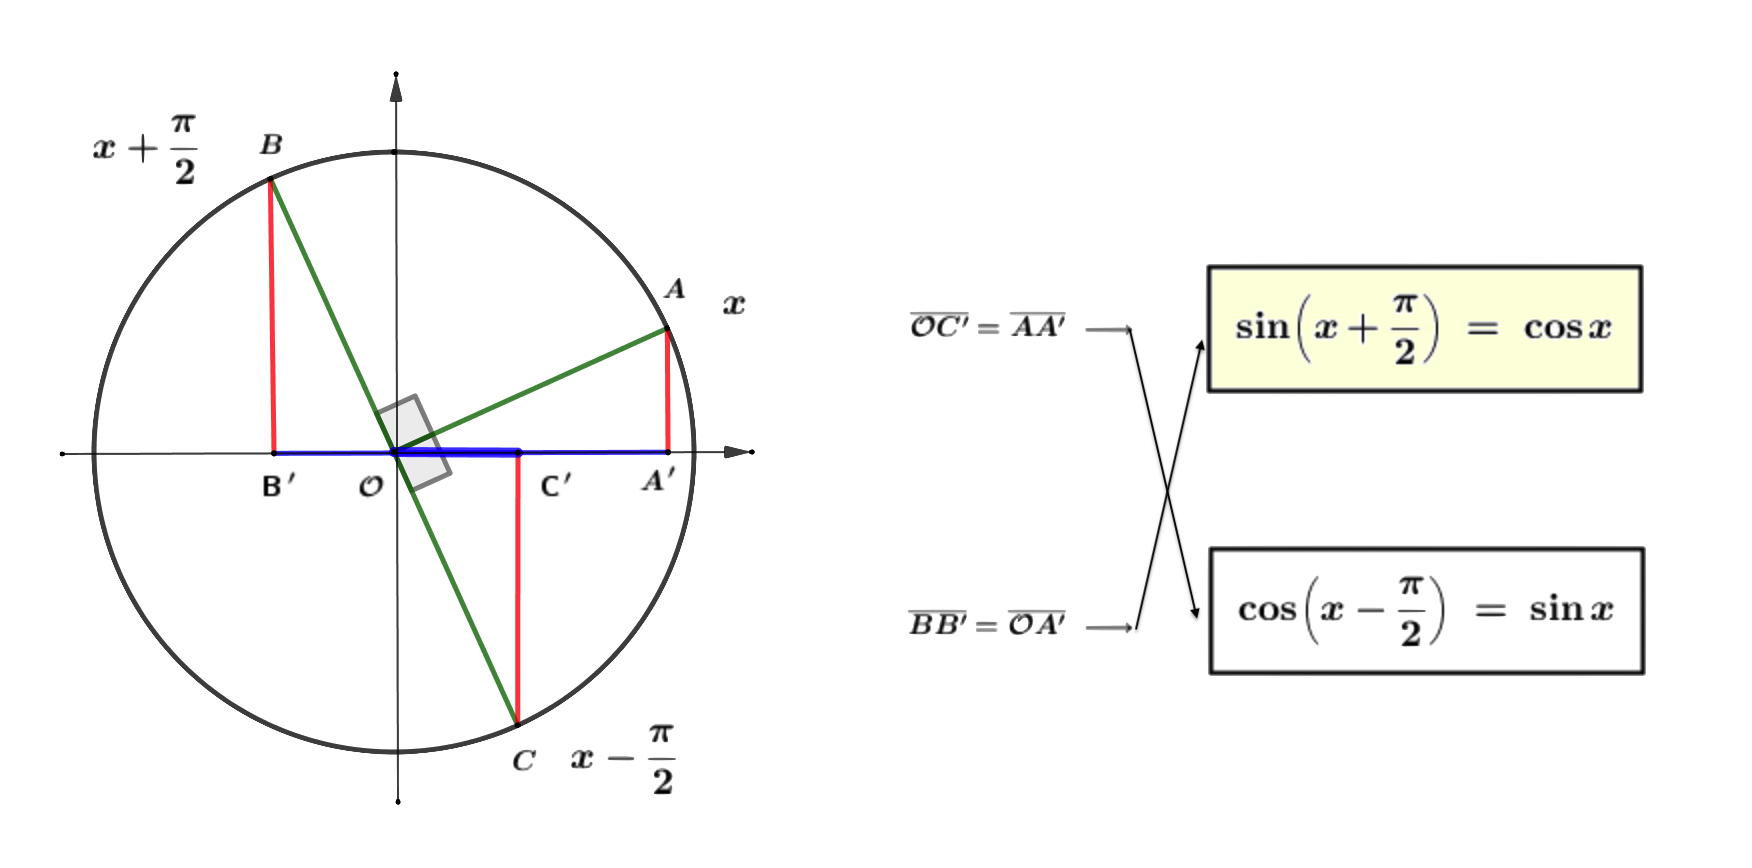
\includegraphics[width=.85\textwidth]{img-rt/rt46.png}
\end{figure}
	Como se aprecia en la figura, el coseno se puede escribir en función de senos y el seno en función de cosenos. También se puede observar en las gráficas de seno y coseno, una está desplazada respecto de la otra $\pi/2$. Será importante recordar que:
	
	$$ \boldsymbol{ \sin(x+\pi/2)=\cos x \, ; \qquad  \qquad \cos(x-\pi/2)=\sin x }$$
\end{cuadro-naranja}






%********************************************************************
\vspace{1cm}
\section{Correspondencias inversas de las funciones trigonométricas}

\begin{tikzpicture}
	\fill [left color=red!50, right color=teal!50] (0,0) rectangle (3.5,.1);
	\fill [left color=teal!50, right color=blue!50] (3.5,0) rectangle (7.5,.1);
	\end{tikzpicture}
\vspace{0.5cm}

Aunque los conceptos que aquí veamos serán desarrollados con mayor profundidad en la parte de \emph{`Cálculo'}, esbozaremos los conceptos de correspondencias inversas de las funciones trigonométricas arcoseno, arcocoseno y arcotangente.

\textcolor{gris}{Puesto que las funciones trigonométricas son \emph{no-inyectivas}, sus inversas no serán funciones matemáticas, por eso hablamos de correspondencias inversas de las funciones trigonométricas.}\footnote{ $\ $ Estos conceptos se desarrollarán el la parte de \emph{`Cálculo'}}

A la correspondencia inversa de la función seno se le llama \emph{arcoseno} ($\asin x \text{ o } \mathrm{arcsin} x$). Puesto que el seno no es inyectivo, en general habrá más de un ángulo para un valor del seno dado.\footnote{ $\ $ Estos conceptos se desarrollarán el la parte de \emph{`Cálculo'}}. Análogamente hablaremos de \emph{arcocoseno} ($\acos x \text{ o } \mathrm{arccos} x$) y \emph{arcotangente} ($\atan x \text{ o } \mathrm{arctan} x$).


\begin{miejemplo}

Con calculadora:   $\qquad \sin 37^o=0.6018 ;\qquad \cos 253^o=-0.2924 ;\qquad \tan 313^o=-1.0724$	

\vspace{2mm} Ahora, al revés,$\ \text{ si } \sin \theta=0.6018 \ \to \ \theta= \asin 0.6018=\begin{cases}\ 37^o \text{ calculadora} \\ \ \theta=180-37=143^o \end{cases}$

\vspace{2mm} Para poder discernir cual es el ángulo buscado necesitaríamos de más información, como en qué cuadrante está el ángulo buscado.

\vspace{2mm} Los ángulos que suman $180^o$ tienen el mismo seno. La calculadora ha proporcionado uno de ellos pero nosotros tenemos que encontrar el otro. Y todo ello en la primera vuelta (de 0 a 360 grados), pero se pueden dar más vueltas. Por ello diremos que:

$$\sin \theta = 0.6018 \ \to \ \theta = \asin 0.6018 \ = \begin{cases} \ 37^o + 360\cdot k \ \\ \ 143^o+360\cdot k \end{cases} \quad \forall k\in \mathbb N$$

Decimos que el arcoseno de 0.6018, el arco (ángulo) cuyo seno vale 0.6018, es 37$^o$ o 143$^o$; en la primera vuelta (de 0 a 360$^o$)

\vspace{2mm} Análogamente:

$$\theta\ = \ \acos (-0.2924) = \begin{cases} \ \theta=107^o \text{\ (calculadora)} \\ \ 360-107=253^o \end{cases} \ \textcolor{gris}{(+360\cdot k)}$$

Los ángulos opuestos tienen los mismo cosenos.

\vspace{2mm} Por último:

$$\theta\ = \ \atan (-1.0724)= \begin{cases} \ -47^0 \text{ (calculadora) }=-47+360=313^o  \\ \ 313-180=133^o \end{cases}  \textcolor{gris}{(+360\cdot k)}$$

\vspace{2mm} Los ángulos que se diferencian en $180^o$ tienen las mismas tangentes.

\vspace{4mm} Las siguientes imágenes muestran como hemos calculado en los ejemplos anteriores el arcoseno, el arcocoseno y la arcotangente.
\begin{figure}[H]
	\centering
	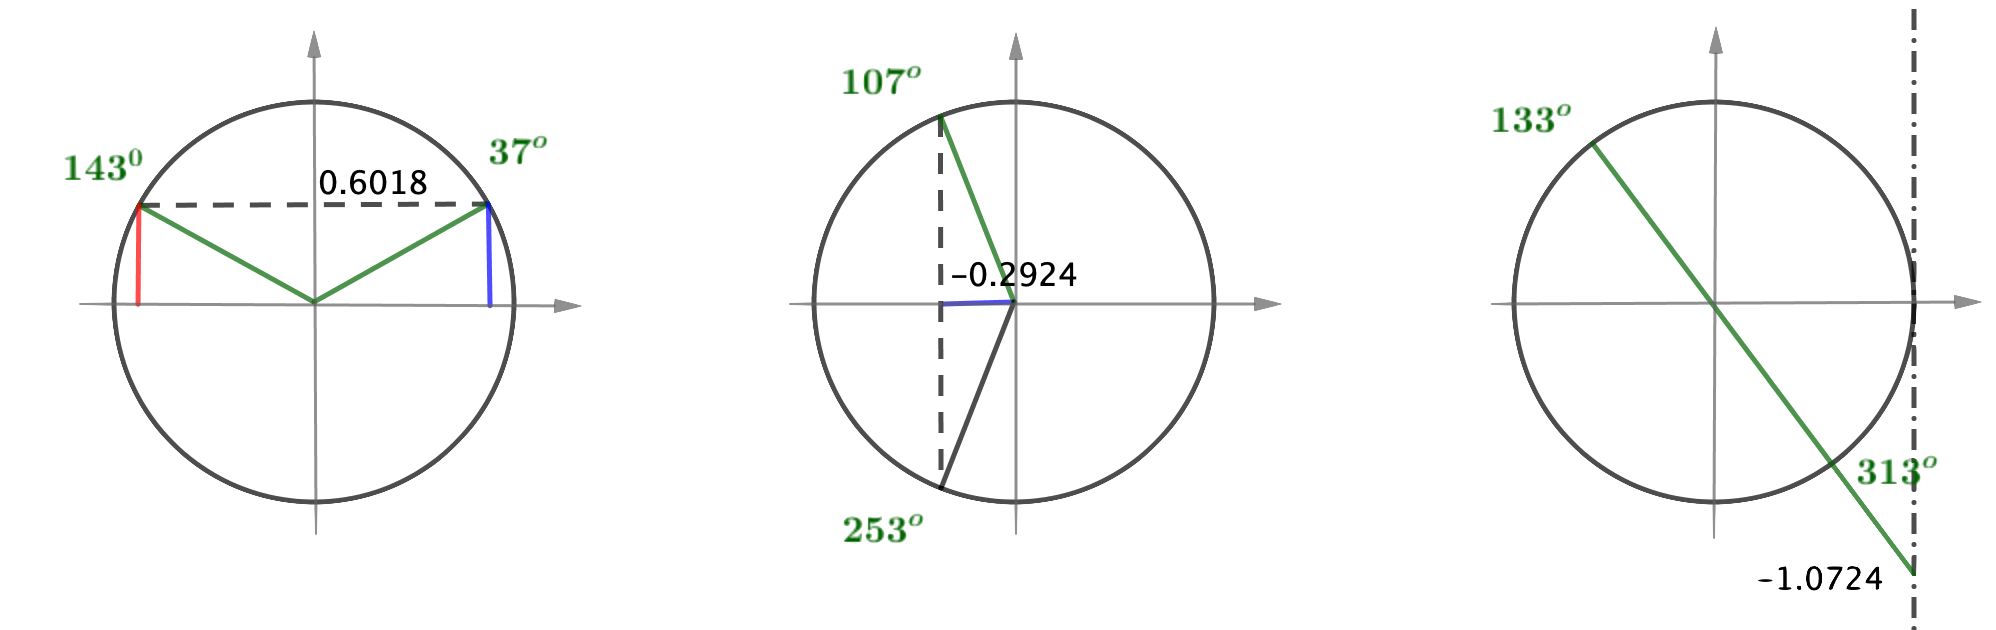
\includegraphics[width=1\textwidth]{img-rt/rt28.png}
\end{figure}
\end{miejemplo}

\vspace{2mm}

$$\subrayado {\ \boldsymbol{ \sin x = y \ \leftrightarrow \ x=\asin y } \ }; \quad 
\subrayado {\ \boldsymbol{ \cos x = y \ \leftrightarrow \ x=\acos y } \ };\quad
\subrayado {\ \boldsymbol{ \tan x = y \ \leftrightarrow \ x=\atan y } \ }$$

Las funciones trigonométricas y sus correspondencias inversas son, efectivamente, inversas las unas de las otras: 

\vspace{2mm}

Veamos que $\quad \sin(\asin x)=x$:

\hspace{1cm} Llamando $\ y=\asin x \ \to \ x=\sin y \ \Rightarrow \ \sin(\asin x)=\sin (y) = x$

Veamos que $\quad \asin (\sin x)=x$:

\hspace{1cm} Llamando $\ y=\sin x \ \to \ \asin (y)= x \ \Rightarrow \  \asin(\sin x)=\asin (y)=x$

Y de forma análoga para $\cos x \text{ y } \acos x$ así como $\tan x \text{ y } \atan x$  


$$\subrayado{\ \boldsymbol{
\sin(\asin(x)) \ = \ x \ = \ \asin(\sin x); \qquad \cos(\acos(x)) \ = \ x \ = \  \acos(\cos x);
} \ }$$ 
\vspace{-5mm}
$$\subrayado{\ \boldsymbol{
\tan(\atan(x)) \ = \ x \ = \ \atan(\tan x)
} \ }$$

\vspace{3mm} Con mayor precisión (se verá con mayor detalle en la parte de cálculo):
\begin{multicols}{2}
$$\sin(\asin x) \ = \ x \quad x\in [-1,1]$$

$$\asin(\sin x) \ = \ x \quad x\in [-\pi/2,\pi/2]$$	
\begin{figure}[H]
	\centering
	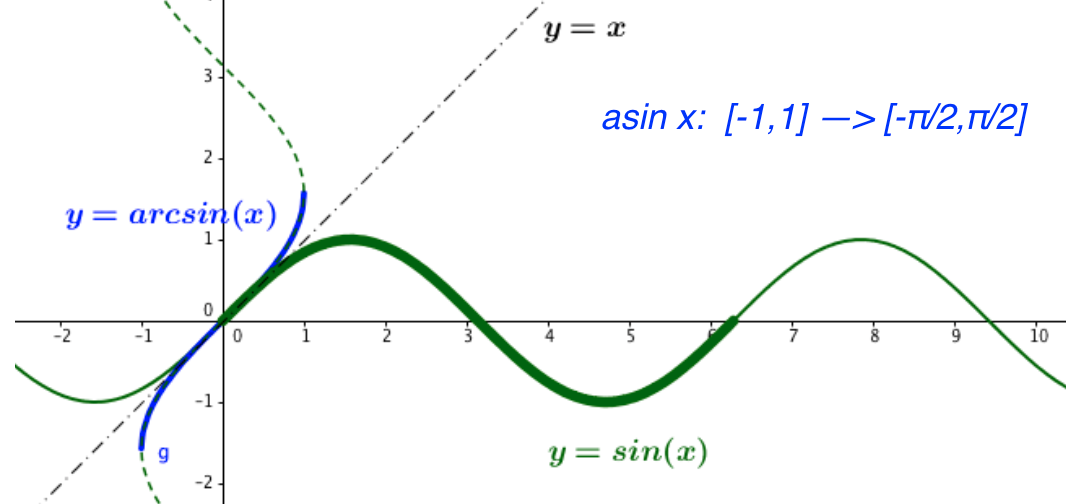
\includegraphics[width=.5\textwidth]{img-rt/rt51.png}
\end{figure}
\end{multicols}


\begin{multicols}{2}
$$\cos(\acos x) \ = \ x \quad x\in [-1,1]$$

$$\cos(\acos x) \ = \ x \quad x\in [0,\pi]$$	
\begin{figure}[H]
	\centering
	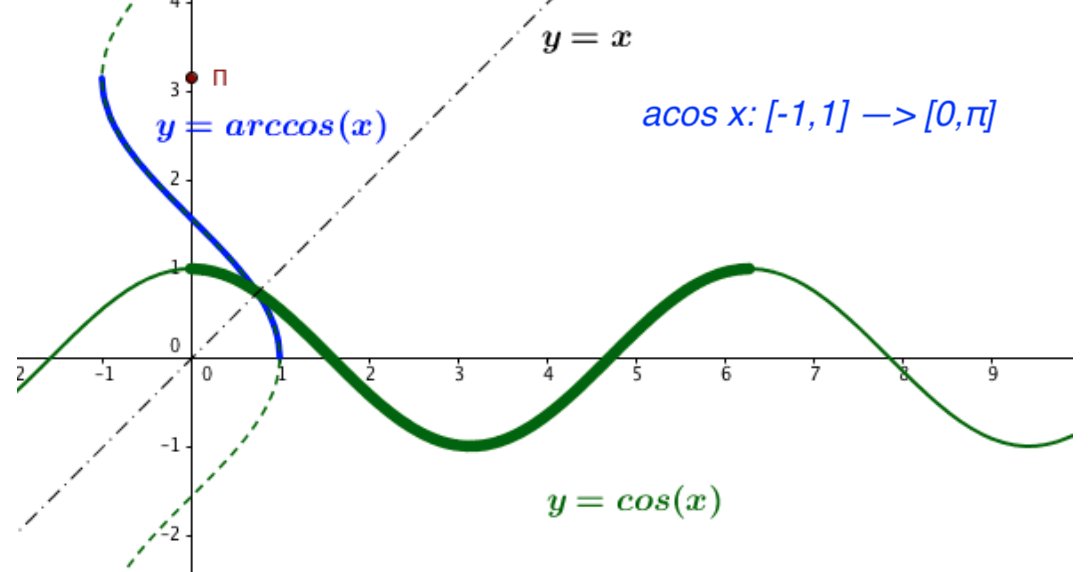
\includegraphics[width=.5\textwidth]{img-rt/rt52.png}
\end{figure}
\end{multicols}


\begin{multicols}{2}
$$\tan(\atan x) \ = \ x \quad \forall x]$$

$$\atan(\tan x) \ = \ x \quad x\in ]-\pi/2,\pi/2[$$	
\begin{figure}[H]
	\centering
	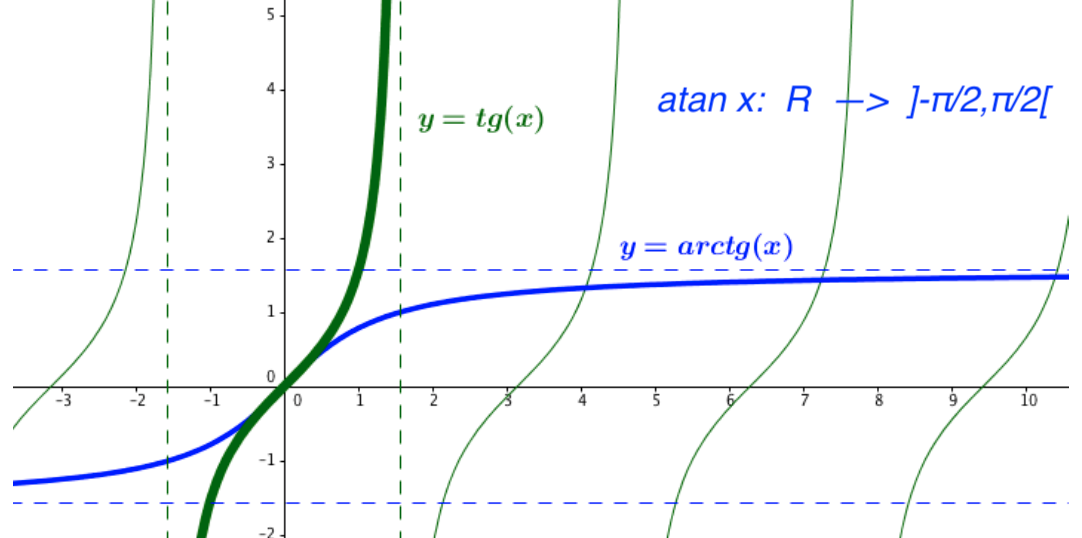
\includegraphics[width=.5\textwidth]{img-rt/rt53.png}
\end{figure}
\end{multicols}

\vspace{5mm} %%%%%%
\underline{Propiedades importantes}: $\qquad \boxed{ \ \boldsymbol{ \cos(\asin x) \ = \ \sqrt{1-x^2} \ = \ \sin(\acos x) } \ } \qquad x\in[-1,1]$

\underline{Demostraciones}: 

\hspace{2cm} $\triangleright \quad \cos(\asin x)=\sqrt{1-\sin^2(\asin x)}=\sqrt{1-(\sin(\asin x))^2}=\sqrt{1-x^2}$

\hspace{2cm} $\triangleright \quad \sin(\acos x)=\sqrt{1-\cos^2(\acos x)}=\sqrt{1-(\cos(\acos x))^2}=\sqrt{1-x^2}$


\vspace{5mm} %%%%%%

\begin{miejemplo}

$\cos \left(\, \asin \left(\,  \dfrac{\sqrt{3}}{4} \, \csc \left(\, \atan \left(\, \dfrac{\sqrt{3}}{\sqrt{2}}\, \sec \dfrac \pi 4 \, \right) \, \right)	\, \right) \, \right)=
\cos \left(\, \asin \left(\,  \dfrac{\sqrt{3}}{4} \, \csc \left(\, \atan \left(\, \dfrac{\sqrt{3}}{\sqrt{2}}\, \dfrac{2}{\sqrt{2}} \, \right) \, \right)	\, \right) \, \right)=
\cos \left(\, \asin \left(\,  \dfrac{\sqrt{3}}{4} \, \csc \left(\, \atan  \sqrt{3} \,  \right)	\, \right) \, \right)=
\cos \left(\, \asin \left(\,  \dfrac{\sqrt{3}}{4} \, \csc \dfrac \pi 3 \, \right)\, \right)=
\cos \left(\, \asin \left(\,  \dfrac{\sqrt{3}}{\sqrt{4}} \dfrac{2}{\sqrt{3}} \, \right)\, \right)=
\cos \left(\, \asin \dfrac 1 2 \right)=\cos \dfrac \pi 6 =\dfrac{\sqrt{3}}{2}$
\end{miejemplo}



\begin{miejercicio}

Calcula $\qquad a)\ \ \sin(\asin 12/13) \qquad \qquad b)\ \ 	\cos (\atan(5/2))$

\rule{250pt}{0.1pt}

\begin{multicols}{2}
\begin{figure}[H]
	\centering
	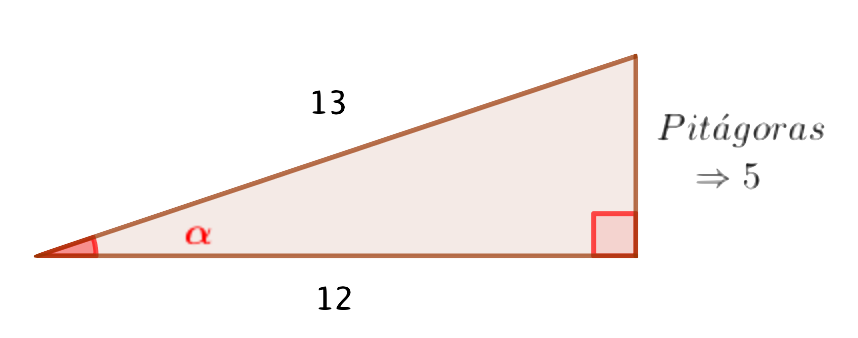
\includegraphics[width=.45\textwidth]{img-rt/rt43.png}
\end{figure}

	\vspace{2mm} $\acos (12/13)=\alpha \ \leftrightarrow \ \cos \alpha=12/13$
	
	\vspace{2mm} de la figura: 
	
	\vspace{2mm} $\sin(\acos(12/13))=\sin \alpha= 5/13$	
\end{multicols}

\begin{multicols}{2}
$\quad$

\vspace{4mm}$\atan(5/2)= \alpha \ \leftrightarrow \ \tan(\alpha)=5/2$

\vspace{2mm}de la figura:

\vspace{2mm}$\cos(\atan(5/2))=\cos(\alpha)=\dfrac 2{\sqrt{29}}=\dfrac{2\sqrt{29}}{29}$
\begin{figure}[H]
	\centering
	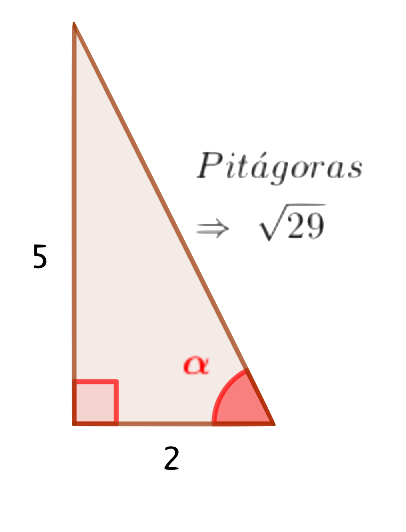
\includegraphics[width=.25\textwidth]{img-rt/rt44.png}
\end{figure}
\end{multicols}	
\end{miejercicio}


\begin{miejercicio}

Calcula: $\qquad \tan \left( \asin \dfrac 2 3 \right) \, \cdot \, \cot \left( \acos \dfrac 1 3 \right)$

\rule{250pt}{0.1pt}

\begin{figure}[H]
	\centering
	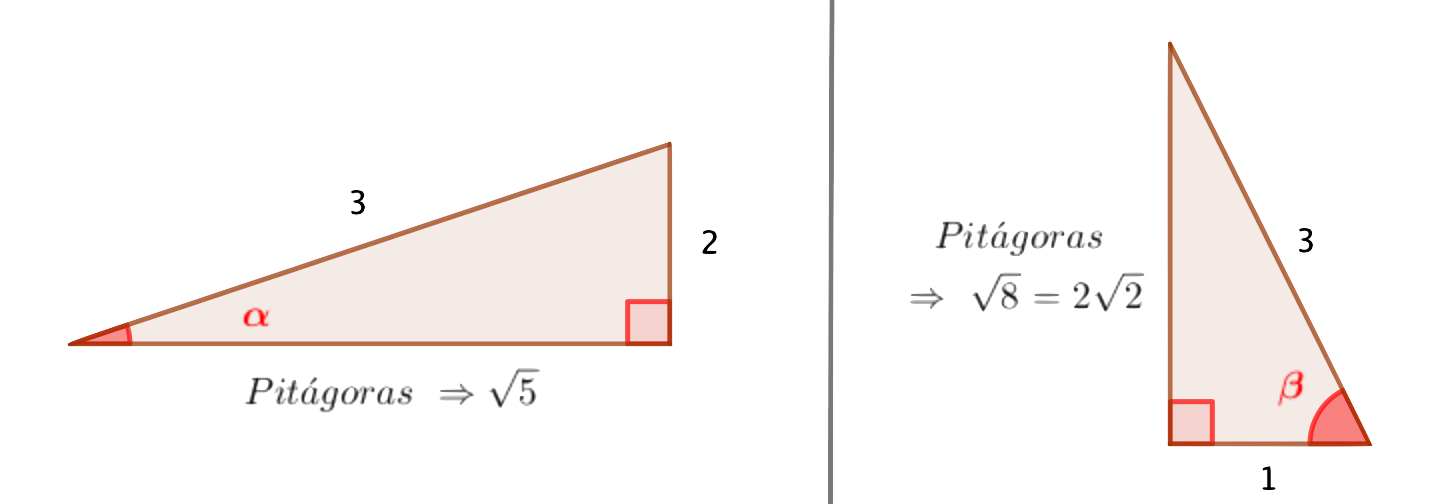
\includegraphics[width=.75\textwidth]{img-rt/rt45.png}
\end{figure}

\begin{multicols}{2}
\vspace{2mm} $\asin (2/3)=\alpha \ \leftrightarrow \ \sin \alpha=2/3$

\vspace{2mm} $\tan(\asin(2/3))=\tan(\alpha)=(\text{figura})=2/\sqrt{5}$

\vspace{2mm} $\acos(1/3)=\beta \ \leftrightarrow \ \cos \beta=1/3$

\vspace{2mm} $\small{\cot(\acos(1/3))=\cot(\beta)=(\text{figura})=1/(2\sqrt{2})}$
\end{multicols}

Finalmente: $\qquad \tan \left( \asin \dfrac 2 3 \right) \, \cdot \, \cot \left( \acos \dfrac 1 3 \right) \ = \ \dfrac {2} {\sqrt{5}} \dfrac{1}{2\sqrt{2}}\ = \  \dfrac {1}{\sqrt{10}}\ = \ \dfrac{\sqrt{10}}{10}$
	
\end{miejercicio}

\vspace{5mm}

\begin{cuadro-naranja}
	OBSERVACIÓN:  Todos los problemas que hemos estado haciendo se podrían resolver más rápidamente usando la calculadora, pero hemos optado por hacerlos sin usarla para familiarizarnos con las propiedades de las funciones trigonométricas lo que nos será de gran utilidad en el cálculo simbólico.
	
	\vspace{5mm}
	
	\begin{cuadro-gris}
	Dada $\cos \alpha=-3$, con $270<\alpha<360$, calcula $\sec(180+\alpha)$
	
	\vspace{5mm} Si $\cot \alpha = -3 \ \to \ \tan \alpha=-1/3\, , \ $ con la calculadora  
	
	$\alpha=\atan(-1/3)= \ \begin{cases} 
	\ -18.4=-18.4+360=341.6 \\ \ 341.6-180=161.6 \end{cases}$

Como  $270<\alpha<360$, entonces $\alpha=341. 6 \ \to \ \sec(180+\alpha)=\sec(180+341.6)=\sec(521.6)=\sec(521.6-360)=\sec(161.6)=\dfrac{1}{\cos(161.6)}=\dfrac{1}{-0.949}=-1.05$
	\end{cuadro-gris}
	
	\begin{cuadro-gris}
		Calcula $\qquad \tan \left( \asin \dfrac 2 3 \right) \, \cdot \, \cot \left( \acos \dfrac 1 3 \right)$
		
		\vspace{5mm}
		Calculadora: $\asin (2/3) = 41.81^o; \qquad \acos(1/3)=70.53^o\, , \ $ luego,
		
		$\tan \left( \asin \dfrac 2 3 \right) \, \cdot \, \cot \left( \acos \dfrac 1 3 \right)= \tan(41.81)\cdot \cot(70.53)= 0.89 \cdot \dfrac{1}{2.83}=0.31$
		
	\end{cuadro-gris}

\end{cuadro-naranja}



%********************************************************************
\vspace{1cm}
\section{Ecuaciones trigonométricas - I/II}

\begin{tikzpicture}
	\fill [left color=red!50, right color=teal!50] (0,0) rectangle (3.5,.1);
	\fill [left color=teal!50, right color=blue!50] (3.5,0) rectangle (7.5,.1);
	\end{tikzpicture}  \hspace{1cm} \footnote{$\ $ Se ampliará en próximos temas}
\vspace{0.5cm}



Las ecuaciones trigonométricas son ecuaciones en las que la incógnita aparece en una función trigonométrica (normalmente en el seno, el coseno o la tangente). Por lo tanto, para resolver ecuaciones trigonométricas se deben utilizar las identidades trigonométricas.


Para resolver una ecuación trigonométrica se deben hacer los siguientes pasos:

\begin{itemize}
\item Aplicar las identidades trigonométricas hasta obtener una sola función trigonométrica (seno, coseno, tangente,…) en la ecuación y despejar.
\item Hacer la inversa de la función trigonométrica (arcoseno, arcocoseno, arcotangente…)
\item Hallar todos los ángulos que son solución de la ecuación trigonométrica. En las ecuaciones trigonométricas intervienen funciones trigonométricas, que son periódicas y por tanto sus soluciones se pueden presentar en uno o en dos cuadrantes y además se repiten en todas las vueltas.
\end{itemize}

A veces no se puede obtener una sola función trigonométrica en la ecuación, en tal caso normalmente se debe extraer (o sacar) factor común. Pero no te preocupes, para que puedas ver exactamente cómo se hacen las ecuaciones trigonométricas, hemos resuelto un ejemplo paso a paso a continuación. También encontrarás más ecuaciones trigonométricas resueltas al final de esta página.

\vspace{4mm}
\begin{miejercicio}

Resuelve las ecuaciones: 

\begin{multicols}{2}
\vspace{2mm} $a)\ \ \tan x + 5(\tan x + 3)=7\tan x - 4$

\vspace{2mm} $b)\ \ 2\sin^2 x+1=\cos^2 x+3 $

\vspace{2mm} $c)\ \ 2(\cos x-7)=7(\sin x-2)$

\vspace{2mm} $d)\ \ 5+4\cos x=4\sin^2 x$	
\end{multicols}


\rule{250pt}{0.1pt}	

\vspace{4mm} $\triangleright \ \ a)\quad \tan x + 5(\tan x + 3)=7\tan x - 4 \ \to \ \tan x=19 \ \to $

\vspace{2mm}$\to \ x=\atan 19 = \begin{cases} \ 87^o+660\, k \\ \ 103^o +360 \, k \end{cases} \forall k \in \mathbb R$



\vspace{4mm} $\triangleright \ \ b)\quad 2\sin^2 x+1=\cos^2 x+3 \ \to \ 2\sin^2 x+1=(1-\sin^2 x) +3 \ \to \ 3\sin^2 x=3 \ \to \ $

\vspace{2mm}$\to \ \sin^2 x=1 \ \to \ \sin x=\pm 1 \ \to \begin{cases}
 \ x=\asin 1  &\to \ x=90^o+360\, k
 \\
 \ x=\asin (-1) &\to \ x=270^o+360\, k 
 \end{cases} \quad \forall k \in \mathbb R$


\vspace{4mm} $\triangleright \ \ c)\quad 2(\cos x-7)=7(\sin x-2)  \ \to \ 2\cos x - \cancel{14}=7\sin x - \cancel {14}$

\vspace{2mm} Como $\cos x\neq 0$, podemos dividir toda la expresión por $\cos x$

\vspace{2mm} \textcolor{gris}{$si \cos x=0 \ \to \ 0=7\sin x\ \to \ \sin x = 0 \ \Rightarrow \ \nexists x\  / \ \cos x=0 \ \wedge \ \sin x=0$ }

\vspace{2mm} Luego $\ \ 2=7\tan x \ \to \ \tan x=2/7 \ \to \ x=\atan (2/7)=\begin{cases}
\ 15.95^o+360\, k \\ \ 195.95^o+360\, k	
\end{cases} \quad \forall k \in \mathbb R $


\vspace{2mm}

\vspace{4mm} $\triangleright \ \ d)\quad 5+4\cos x=4\sin^2 x \ \to \ 5+4\cos x=4(1-\cos^2 x) \ \to \ 4\cos^2 x+4\cos x+1=0$

\vspace{2mm}$\cos x=\dfrac{-4\pm \sqrt{16-16}}{8}=-\dfrac 1 2 \to  \ x=\acos (-1/2)= \begin{cases}
 	\ 120^o+360\, k \\ \ 240^o+360\, k
 \end{cases}\quad \forall k \in \mathbb R $

\begin{figure}[H]
	\centering
	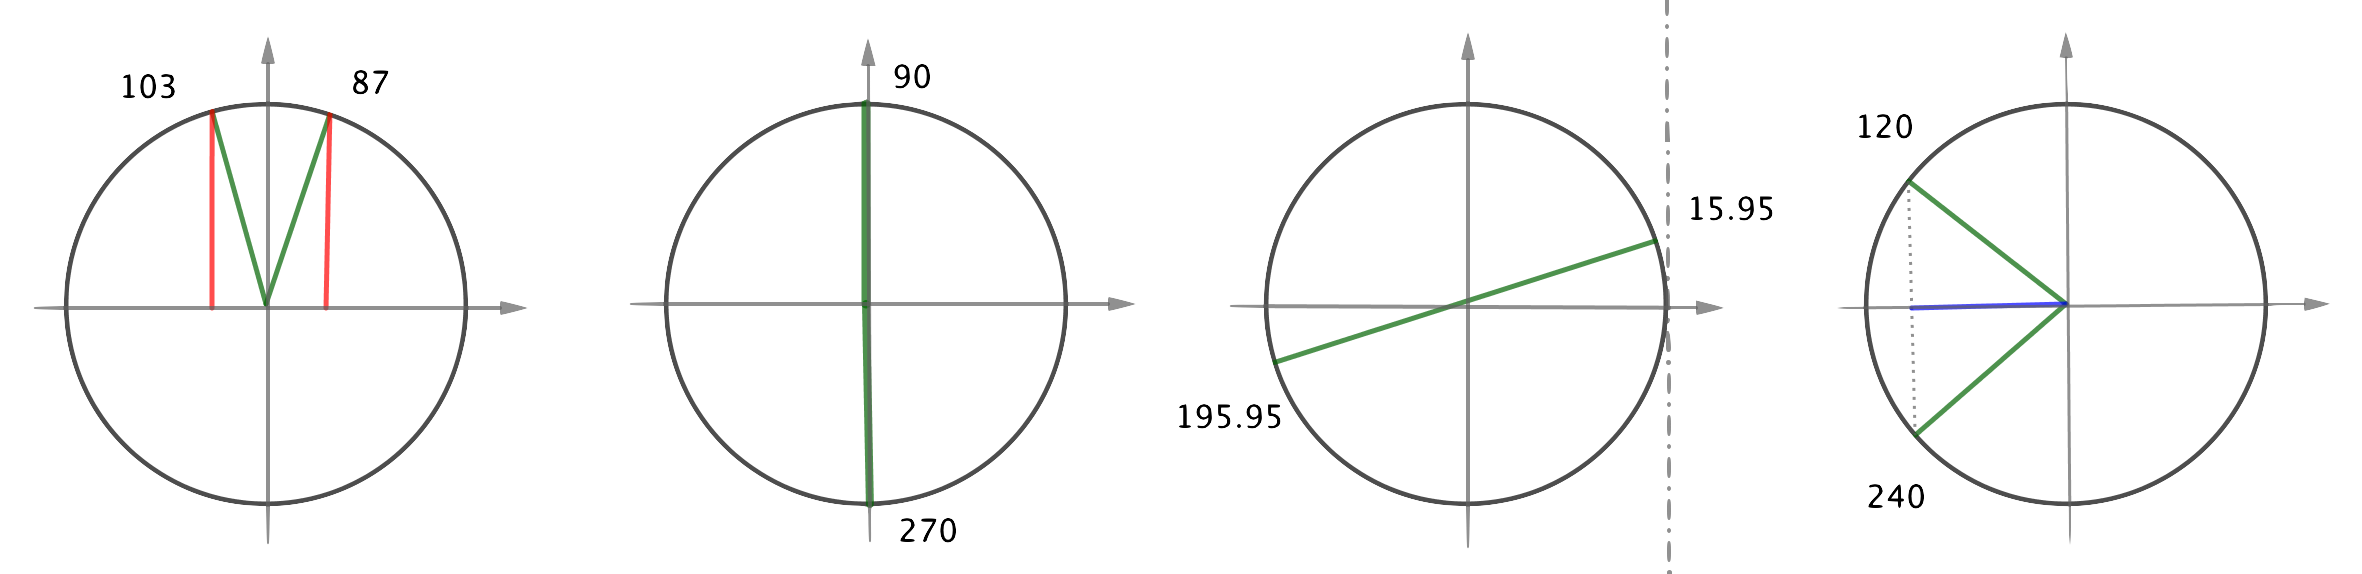
\includegraphics[width=1\textwidth]{img-rt/rt30.png}
\end{figure}

\end{miejercicio}
%\vspace{5mm}

\begin{destacado}
--- Los ángulos que tiene los mismos senos suman $180^0\, : \ \ \alpha+\beta=180 \ $ (suplementarios)

--- Los ángulos que tiene los mismos cosenos suman $360^o\, : \ \ \alpha+\beta=360\ $ (opuestos)	

--- Los ángulos que tienen. las mismas tangentes se diferencian en $180^o\, : \ \ \alpha-\beta=180\ $
\end{destacado}

\begin{miejercicio}

Resuelve $\ \sin x + \cos x = 1$

\rule{250pt}{0.1pt}

\vspace{3mm} En esta ocasión, para reducir a una sola RT,  no nos queda 	más remedio que hacer que aparezca una ecuación irracional,; tendremos que aislar y elevar al cuadrado

$\sin^2x+\cos^2x=1 \ \to \ \cos^2x=1-\sin^2 x\  \to \ \cos x=\sqrt{1-\sin^2 x}$

$\sin x+\cos x=1 \ \to \ \sin x+\sqrt{1-\sin^2 x}=1 \ \to \ (1-\sin x )^2= \left( \sqrt{1-\sin^2 x} \right)^2$

$1+\sin^2 x-2\sin x=1-\sin^2 x \ \to \ 2\sin^2 x-2\sin x=0=2\sin x(1-\sin x) \ \to$

$\to \ \begin{cases}
 \ \sin x =0 &\to \begin{cases} \ x=0+360k \\ \	x=180+360k \end{cases} \\
 \ 1-sin x =0 \ \to \ \sin x=1 &\to \begin{cases} \ x=90+260 k \end{cases}
  \end{cases}$
  
 Al elevar al cuadrado tenemos que comprobar si las tres soluciones obtenidas satisfacen la ecuación original y sí lo hacen, las tres son buenas.
 
\vspace{5mm} \underline{De otro modo}: Si elevamos al cuadrado la ecuación original,

$(\sin x+\cos x)^2=1^2 \ \to \ \sin^2 x + \cos^2 x+2\sin x \cos x=1 \to \text{ (relación fdmtal. trig.) } \to 1+2 \sin x \cos x = 1 \to 2 \sin x \cos x=0 \ \to \ \sin x \cdot \cos x=0 \ \Rightarrow $


\begin{multicols}{2}
$\Rightarrow \ \  \sin x = 0   \ \to \ \begin{cases} \ \ x=0+360k \\ \ x=180+360k \end{cases} $

$\Rightarrow \ \ \cos x = 0	\ \to \  \begin{cases} \ \ x=90+360k \\ \ x=270+360k \end{cases} $
\end{multicols}
 
Al haber elevado al cuadrado para resolver la ecuación se han podido introducir soluciones extrañas, por lo que hay que comprobar cada una de ellas en la ecuación inicial resultando que $x=270+360k$ no la cumple, por lo que las soluciones serán:
$\ x=0+360k,\ \ x=90+360k \ \text{ y } \ x=180+360k$

\end{miejercicio}



%********************************************************************
\vspace{1cm}
\section{Resolución de triángulos rectángulos}

\begin{tikzpicture}
	\fill [left color=red!50, right color=teal!50] (0,0) rectangle (3.5,.1);
	\fill [left color=teal!50, right color=blue!50] (3.5,0) rectangle (7.5,.1);
	\end{tikzpicture}
\vspace{0.5cm}

Resolver un triángulo (rectángulo en este tema) consiste en calcular la medida de sus tres lados y de sus tres ángulos.


Para resolver triángulos rectángulos  tendremos en cuenta que:

\begin{itemize}
\item La suma de los dos ángulos agudos es 90$^o$.
\item La suma de dos lados siempre es mayor que el otro lado.
\item Sus lados están relacionados entre sí a través del teorema de Pitágoras.  
\item Los lados y los ángulos se relacionan entre sí a través de las definiciones de las razones trigonométricas.
\end{itemize}


En general, para poder resolver un triángulo necesitamos conocer como mínimo, un lado, puesto que si conociésemos los ángulos y ningún lado, tendríamos infinitos triángulos semejantes. En el caso de los triángulos rectángulos, ya se conoce la medida del ángulo de 90$^o$. Es decir, para resolver un triángulo rectángulo, se necesitan dos datos (además de que hay un ángulo recto) y uno de ellos ha de ser obligatoriamente un lado.


Teniendo en cuenta esto, podemos encontrarnos con dos casos:

--- Si se conocen un lado y un ángulo agudo, las razones trigonométricas nos permitirán hallar los otros dos lados.

--- Si se conocen dos lados, no necesitamos conocer ningún ángulo puesto que aplicando el teorema de Pitágoras podremos hallar el tercer lado. Y a partir de los lados, se calculan las razones y con éstas, los ángulos.

\vspace{5mm}
\begin{miejemplo}

Resuelve los siguientes triángulos rectángulos:	

\begin{figure}[H]
	\centering
	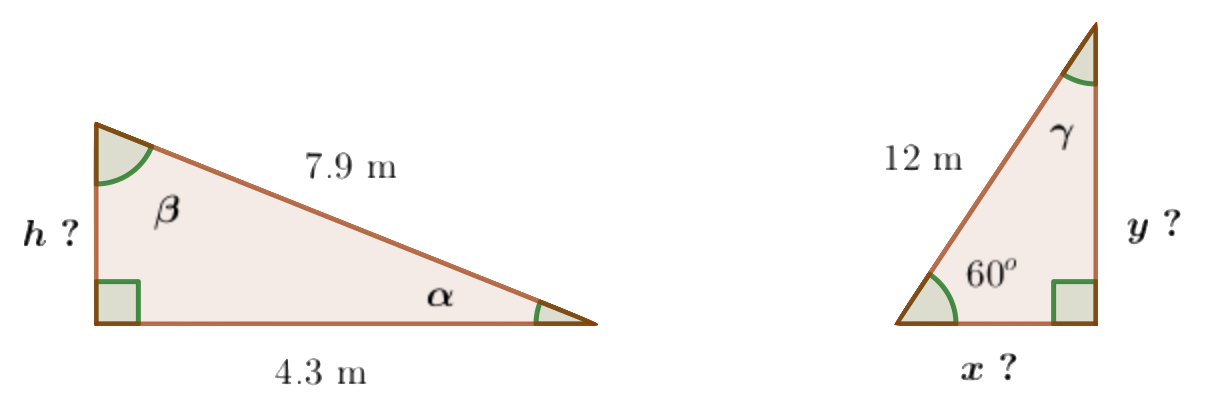
\includegraphics[width=.75\textwidth]{img-rt/rt31.png}
\end{figure}

\vspace{5mm} $\triangleright \ \ $ En el primer triángulo, por el teorema de Pitágoras: $\quad h^2+4.3^2=7.9^2 \ \to \ h= 6.6\ \mathrm{m}$

\vspace{2mm} $\cos \alpha=\dfrac{4.3}{7.9}\ \to \ \alpha=\acos 0.544= 57^o$, en este caso solo hay una solución pues los ángulos de un triángulo rectángulo son agudos (excepto el de 90$^o$, claro). 

\vspace{2mm} Puesto que todos los ángulos de un triángulo suman 180$^o$, tendremos que $\beta+57+90=180 \ \to \ \beta=33^o$ 

\vspace{5mm} $\triangleright \ \ $ En el segundo triángulo, al solo conocer uno de los lados, no podemos acudir a Pitágoras. Puesto que el dato conocido es la hipotenusa, acudimos al seno o al coseno de uno de los ángulos agudos, del de 60$^o$, que es el ángulo conocido.

\vspace{2mm} $\cos 60^0=\dfrac1 2 =\dfrac {\text{cat. cont.}}{\text{hipoten.}}=\dfrac{x}{12} \ \to \ x=12\cdot \dfrac 1 2 = 6\ \mathrm{m};\quad \sin 60=0.87=\dfrac y {12} \ \to \ y=10.4\ \mathrm{m}$

\vspace{2mm} El ángulo $\gamma$ será lo que falte hasta 180: $\quad \gamma+60+90=180 \ \to \ \gamma=30^o$
\end{miejemplo}


\vspace{5mm}
\begin{miejercicio}

\begin{multicols}{2}
$\quad$

Para el siguiente triángulo, calcula:

\vspace{6mm} Altura $h$, longitudes $\overline{BD} \text{ y } \overline{CD}$

\vspace{3mm} Base ($\overline{BC}$) y su área.
\begin{figure}[H]
	\centering
	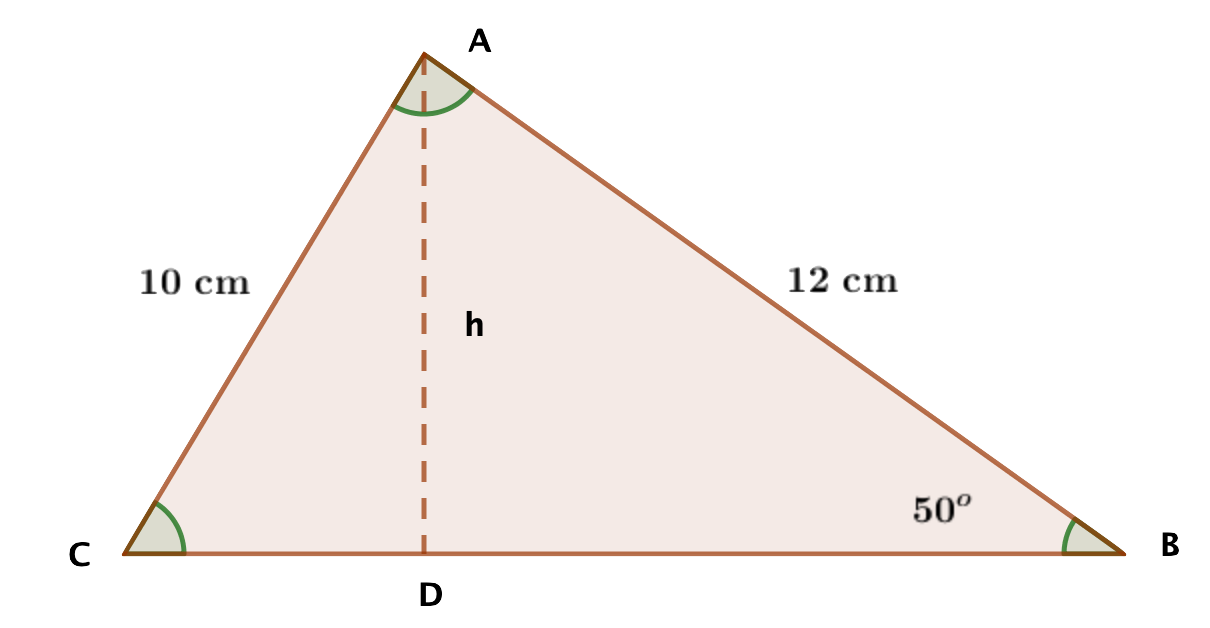
\includegraphics[width=.5\textwidth]{img-rt/rt32.png}
\end{figure}	
\end{multicols}

\vspace{-10mm}%%%%%%%%
\rule{250pt}{0.1pt}	

\vspace{3mm} Triángulo de la derecha: $\ \sin 50=\dfrac h{12} \ \to \ h=12\, \sin 50=9.2 \ \mathrm{cm}$

\vspace{1mm} $\cos 50=\dfrac{\overline{BD}}{12} \ \to \ \overline{BD}=12\, \cos 50=7.7 \ \mathrm{cm}$

\vspace{5mm} Triángulo de la izquierda: $\ 10^2=\overline{CD}+h^2=\overline{CD}+9.2^2 \ \to \ \overline{CD}=3.9 \ \mathrm{cm}$

\vspace{1mm} Base: $\overline{BC}=	\overline{BD}+\overline{CD}=7.7+3.9=11.6 \ \mathrm{cm}$

\vspace{1mm} Área $=\dfrac 1 2 \, \overline{BD}\cdot h=\dfrac 1 2 \cdot 11.6 \cdot 9,2 = 53.4 \ \mathrm{cm}^2$
\end{miejercicio}



\begin{miejercicio}

\begin{multicols}{2}
\vspace{2mm} Desde el suelo vemos el punto más alto de un edificio con un ángulo de 60$^o$. Nos alejamos 6 metros en línea recta y este ángulo es de 50$^o$. ?`Cuál es la altura del edificio?

\begin{figure}[H]
	\centering
	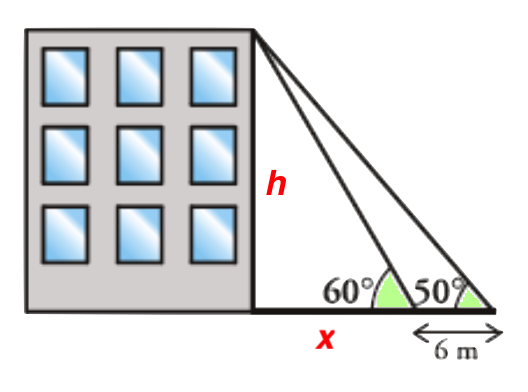
\includegraphics[width=.3\textwidth]{img-rt/rt33.png}
\end{figure}
\end{multicols}
\vspace{-10mm}
\rule{250pt}{0.1pt}	

\vspace{5mm} Realmente tenemos dos triángulos rectángulos, de ángulos agudos desde el suelo de $50^o$ y $60^o$ y catetos contiguos de $6\, \mathrm{m}$ y $6+x\, \mathrm{m}$, respectivamente. Ambos triángulos tienen el mismo cateto opuesto, $h \, \mathrm{m}$. Usando las tangentes:

\vspace{2mm} $\begin{cases}
 	\ \tan 50 = \dfrac{h}{x+6}=1.19 &\to \ h=1.19(x+6) \\ \\
 	\ \tan 60 = \dfrac h x =1.73 &\to \ h=1.73 x
 \end{cases} \ \to \quad 1.19(x+6)=1,73 x \ \Rightarrow \ x=13.24\, \mathrm{m}$
 
 \vspace{2mm}  Finalmente, $\quad h=1.73 \, x =1.73 \cdot 13.24=22.91 \, \mathrm{m}$

\end{miejercicio}

%********************************************************************
\vspace{1cm}
\section{Ejercicios}

\begin{tikzpicture}
	\fill [left color=red!50, right color=teal!50] (0,0) rectangle (3.5,.1);
	\fill [left color=teal!50, right color=blue!50] (3.5,0) rectangle (7.5,.1);
	\end{tikzpicture}
\vspace{0.5cm}

%%%%%
\begin{mipropuesto}

Sabiendo que $\ \sec \alpha=-4\ $	y que $\ 0<\alpha<\pi\ $, calcula: 

\vspace{1mm} $a)\ \ \csc(3\pi/2+\alpha);\quad b)\ \ \sin(\pi/2-\alpha);\quad c)\ \ \tan(2610^o-\alpha); \quad d)\ \ \cos(180+\alpha)$
\end{mipropuesto}

\vspace{-8mm}
\begin{flushright}
\begin{footnotesize} \textcolor{gris}{\rotatebox{180}{ $-4;\ \ -1/4;\ \  -0.26;\quad 1/4$}}	\end{footnotesize}
\end{flushright}



%%%%%
\begin{mipropuesto}

Sabiendo que $\ \tan \alpha=1/2\ $ y que $\ \pi < \alpha < 3\pi/2\ $, calcula:

\vspace{1mm}$a)\ \ \sin(\pi/2+\alpha);\quad b)\ \ \cos(\pi+\alpha);\quad c)\ \ \cot(\pi-\alpha);\quad d)\ \ \cot(360-\alpha)$	
\end{mipropuesto}

\vspace{-8mm}
\begin{flushright}
\begin{footnotesize} \textcolor{gris}{\rotatebox{180}{ $-0.89;\quad 0.89;\quad -2;\quad -2$ }}	\end{footnotesize}
\end{flushright}



%%%%%%%
\begin{mipropuesto}

Simplifica: 

\vspace{1mm} $ a) \ \ \dfrac{(\sin \alpha-\cos \alpha)^2+(\sin \alpha+\cos \alpha)^2}{\csc \alpha \, \tan \alpha} \, ; \qquad b) \ \ \cos^3 \alpha+ \cos^2 \alpha \sin \alpha + \cos \alpha \sin^2 \alpha + \sin^3 \alpha $ 	
\end{mipropuesto}

\vspace{-8mm}
\begin{flushright}
\begin{footnotesize} \textcolor{gris}{\rotatebox{180}{ $2\cos \alpha \qquad b)\ \sin \alpha + \cos \alpha$ }}	\end{footnotesize}
\end{flushright}



%%%%%%%
\begin{mipropuesto}

Simplifica:

\vspace{1mm} $a)\ \ \dfrac{1}{1-\sin \alpha}+\dfrac{1}{1+\sin \alpha}-2\, ;\qquad b)\ \ \dfrac{\sin(\pi+ \alpha)\, \tan \left( \dfrac \pi 2 + \alpha \right) }{ \sec^2 \left( \dfrac \pi 2 + \alpha \right)\, (1-\cos^2 \alpha )\, \cos \alpha }-\cos^2 \left( \dfrac \pi 2 + \alpha \right)$	
\end{mipropuesto}

\vspace{-8mm}
\begin{flushright}
\begin{footnotesize} \textcolor{gris}{\rotatebox{180}{ $-2\sin^2 \alpha;\qquad \cos^2 \alpha$ }}	\end{footnotesize}
\end{flushright}


%%%%%%%
\begin{mipropuesto}

Demuestra:

\vspace{1mm} $a)\ \ \dfrac1{\cos^2 \alpha+\sin^2 \alpha + \tan^2 \alpha}=\cos^2 \alpha\, ; \qquad b)\ \ \dfrac{\sin \alpha \, \cos \alpha}{\sin^2 \alpha - \cos^2 \alpha}=\dfrac{\tan \alpha}{\tan^2 \alpha - 1}$	
\end{mipropuesto}

\vspace{-8mm}
\begin{flushright}
\begin{footnotesize} \textcolor{gris}{\rotatebox{180}{ Sí;	$\quad$ sí}}	\end{footnotesize}
\end{flushright}



\begin{mipropuesto}

 Calcula: $\qquad \sin \left( \, \asin  \, \dfrac{\sqrt{5}}{3} \, \right) $

\end{mipropuesto}

\vspace{-8mm}
\begin{flushright}
\begin{footnotesize} \textcolor{gris}{\rotatebox{180}{  2/3}}	\end{footnotesize}
\end{flushright}


\begin{mipropuesto}

 Calcula: $\qquad \cos^2 \left(\, \asin \dfrac{\sqrt{5}}{3} \, \right)$

\end{mipropuesto}

\vspace{-8mm}
\begin{flushright}
\begin{footnotesize} \textcolor{gris}{\rotatebox{180}{  4/9 }}	\end{footnotesize}
\end{flushright}


\begin{mipropuesto}

 Resuelve: $\qquad \cos \left( x+\dfrac \pi 6 \right)=\dfrac{\sqrt{3}}{2}$

\end{mipropuesto}

\vspace{-8mm}
\begin{flushright}
\begin{footnotesize} \textcolor{gris}{\rotatebox{180}{  $x=2k\pi \quad \wedge \quad x=5\pi/3+2k\pi $  }}	\end{footnotesize}
\end{flushright}


%%%%%%%
\begin{mipropuesto}

Resuelve:

\vspace{1mm} $a)\ \ 3\sec x-3\sin x\tan x=-3\, ; \qquad b)\ \ 2\tan^2 x-1=2\sin^2 x$	
\end{mipropuesto}

\vspace{-8mm}
\begin{flushright}
\begin{footnotesize} \textcolor{gris}{\rotatebox{180}{ $a) \ x=( 90^o,\,  180^o, \, 270^o ) \ (+360k)\, ; \qquad b)\ x=(45^o,\, 135^o,\, 225^o,\, 315^o) \ (+360k)$ }}	\end{footnotesize}
\end{flushright}




%%%%%%%
\begin{mipropuesto}

\begin{multicols}{2}
Dos personas, Alberto (A) y Beatriz (B), están situados cada uno a un lado de un árbol (como indica la figura).

Calcula la altura del árbol y la distancia de cada uno de ellos al árbol.
\begin{figure}[H]
	\centering
	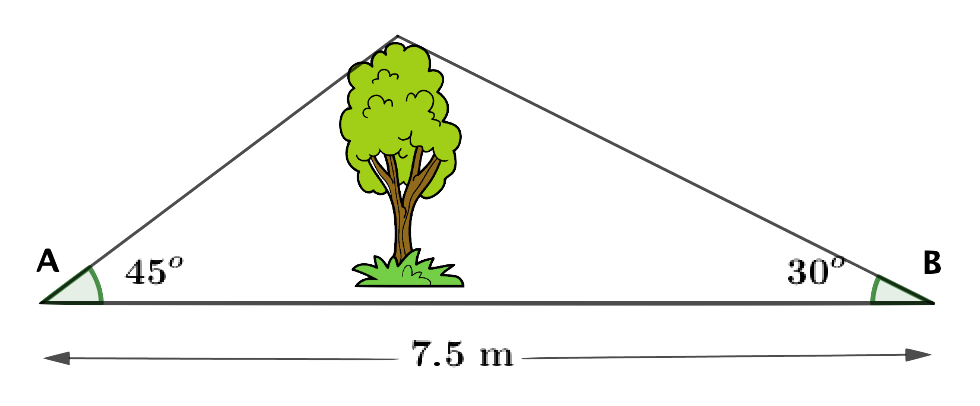
\includegraphics[width=.5\textwidth]{img-rt/rt34.png}
\end{figure}
\end{multicols}
	
\end{mipropuesto}

\vspace{-8mm}
\begin{flushright}
\begin{footnotesize} \textcolor{gris}{\rotatebox{180}{ 2.75m; $\quad$ 2,75 y 4.75 m, respectivamente. }}	\end{footnotesize}
\end{flushright}


%%%%%%%
\begin{mipropuesto}

\begin{multicols}{2}
$\quad$

$\quad$

$\quad$

Calcula la altura de ambos rectángulos.

$\quad$

$\quad$

\begin{figure}[H]
	\centering
	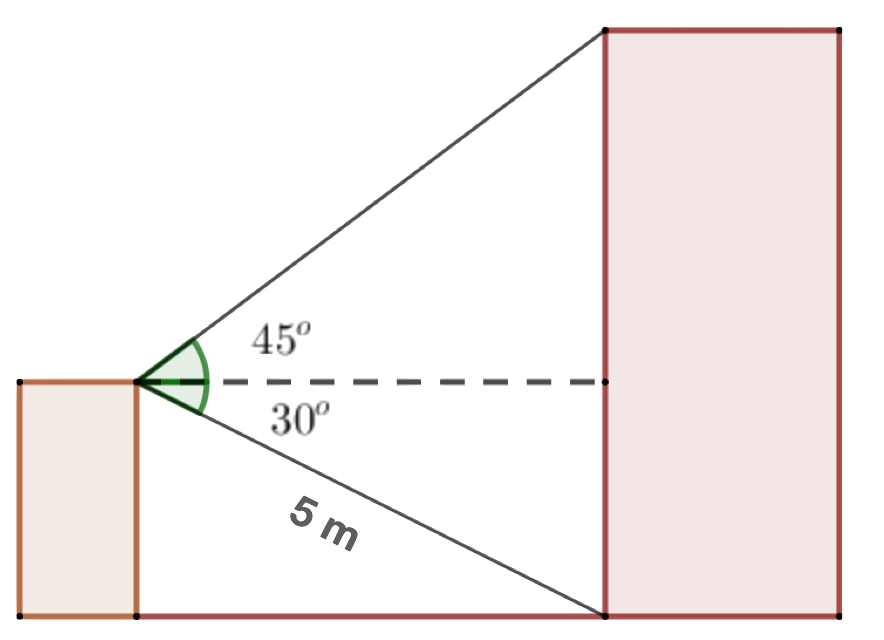
\includegraphics[width=.4\textwidth]{img-rt/rt35.png}
\end{figure}
\end{multicols}
	
\end{mipropuesto}

\vspace{-8mm}
\begin{flushright}
\begin{footnotesize} \textcolor{gris}{\rotatebox{180}{ 2.5 y 6.8 m, respectivamente. }}	\end{footnotesize}
\end{flushright}


\begin{mipropuesto}

 En lo alto de un edificio hay una antena. Desde una distancia de 55 m se ve la base de la antena con un ángulo de elevación de 36$^o$ y el extremo de dicha antena con un ángulo de elevación de 40$^o$. Hallar la altura de la antena.
 
\end{mipropuesto}

\vspace{-8mm}
\begin{flushright}
\begin{footnotesize} \textcolor{gris}{\rotatebox{180}{  6.19 m }}	\end{footnotesize}
\end{flushright}


\begin{mipropuesto}

 Se quiere medir la anchura de un río. Para ello se observa un árbol que está en la otra orilla a la parte más alta y se obtine un ángulo de elevación de 55$^o$. Alejándose 5 m del río en la misma dirección del árbol se vuelve a medir el ángulo de elecvación y se obtiene 42$^o$. Calcula la anchura del río y la altura del árbol.

\end{mipropuesto}

\vspace{-8mm}
\begin{flushright}
\begin{footnotesize} \textcolor{gris}{\rotatebox{180}{  8.53 m y 12.18 m }}	\end{footnotesize}
\end{flushright}




\vspace{5mm}%%%%%%%%

\newpage
$\quad$

\begin{myexampleblock}{Recordatorio: teorema de Thales y semejanza de triángulos}
	
\begin{multicols}{2}
$\quad$

$r \, || \, s\, || \, t$, rectas paralelas que cortan a otras dos $u,\ v$ 

$\Rightarrow \ $ los segmentos que determinan son proporcionales.

$$\dfrac{\ \overline{AB}\ }{\ \overline{A'B'} \ }=\dfrac{\ \overline{BC}\ }{\ \overline{B'C'}\ }=\dfrac{\ \overline{AC}\ }{\ \overline{A'C'}\ }=\dfrac{\ \overline{OA}\ }{\ \overline{OA'}\ }$$
\begin{figure}[H]
	\centering
	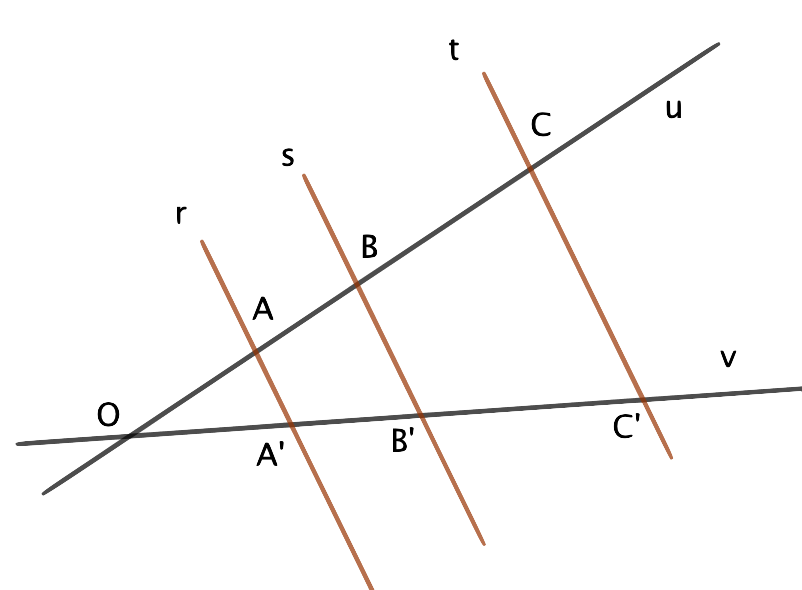
\includegraphics[width=.4\textwidth]{img-rt/rt36.png}
\end{figure}	
\end{multicols}

\begin{multicols}{2}
\begin{figure}[H]
	\centering
	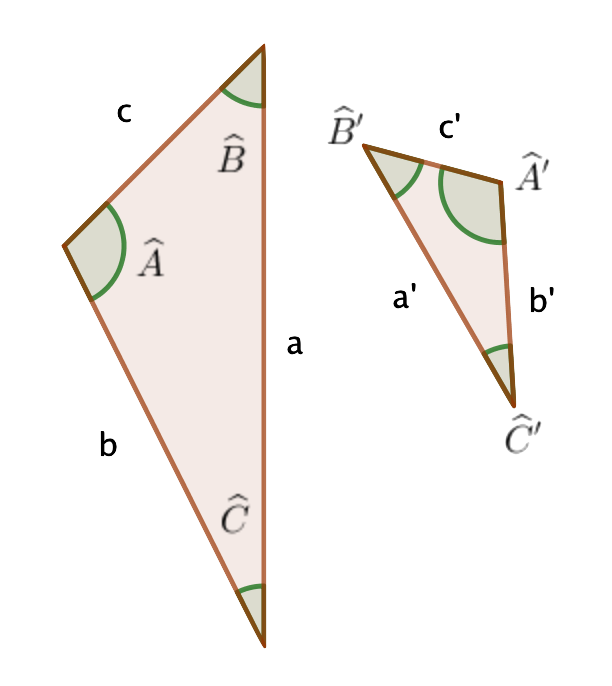
\includegraphics[width=.35\textwidth]{img-rt/rt37.png}
\end{figure}	
$\quad$

\emph{Semejanza de triángulos}:

$\quad$ --- Lados proporcionales:

$$\dfrac{a}{a'}=\dfrac{b}{b'}=\dfrac{c}{c'}$$

$\quad$ --- Ángulos iguales:

$$\widehat{A}=\widehat{A'};\quad \widehat{B}=\widehat{B'}; \quad \widehat{C}=\widehat{C'}$$
\end{multicols}

\begin{multicols}{2}
$\quad$

Dos triángulos con un ángulo común y lados opuestos paralelos están en \emph{posición de Thales}.

$\quad$

\emph{Los triángulos en posición de Thales son semejantes}.
\begin{figure}[H]
	\centering
	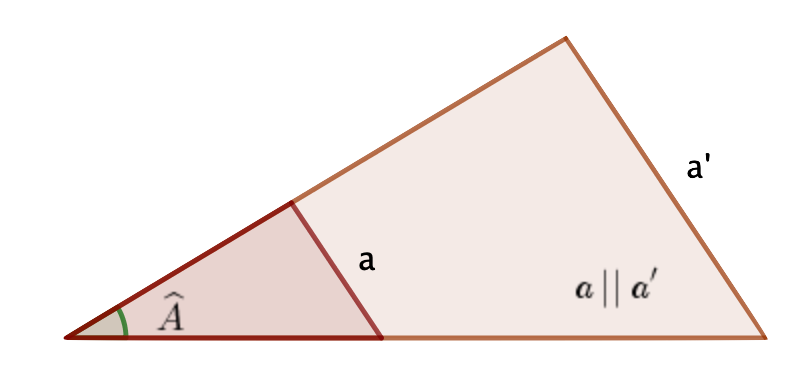
\includegraphics[width=.45\textwidth]{img-rt/rt38.png}
\end{figure}	
\end{multicols}

\emph{Criterios de semejanza de triángulos}.

\vspace{1mm}
1.-Dos triángulos son semejantes si tienen dos ángulos iguales.

2.-Dos triángulos son semejantes si tienen dos lados proporcionales e igual el ángulo que forman.

3.- Dos triángulos son semejante si sus lados son proporcionales.
\end{myexampleblock}


\newpage

%********************************************************************
\vspace{1cm}
\begin{adjustwidth}{50pt}{250pt}
\begin{cuadro-naranja}
\textbf{\huge{Problemas $\boldsymbol{+}$}}\normalsize{$\, $}
\end{cuadro-naranja}	
\end{adjustwidth}

\vspace{5mm}
\begin{enumerate}[\textbf{P$\boldsymbol +$} 1. ]


\item	Demuestra que las siguientes líneas representan las razones trigonométricas que se indican.

\begin{figure}[H]
	\centering
	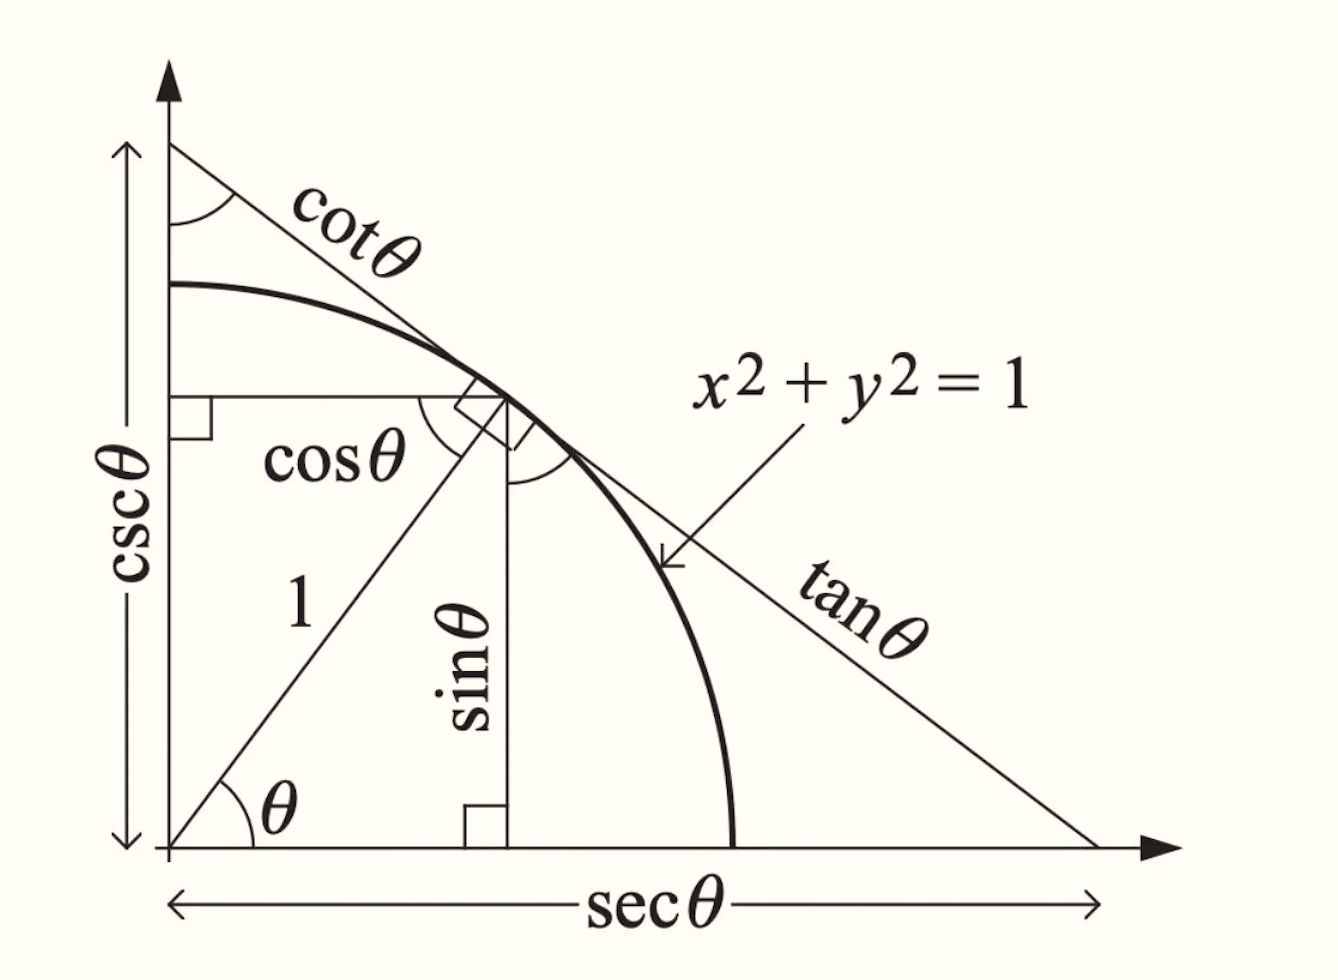
\includegraphics[width=.5\textwidth]{img-rt/rt41.png}
\end{figure}

\vspace{-6mm}
\begin{flushright}
\begin{footnotesize} \textcolor{gris}{\rotatebox{180}{ Semejanza de triángulos. }}	\end{footnotesize}
\end{flushright}

\item	

\begin{multicols}{2}
$\quad$

La figura representa un triángulo equilátero de lado $6$ cm inscrito en un círculo. 

Si el área del círculo es $k\, \pi$ cm$^2$, determina el valor de $k$.

$\quad$
\begin{figure}[H]
	\centering
	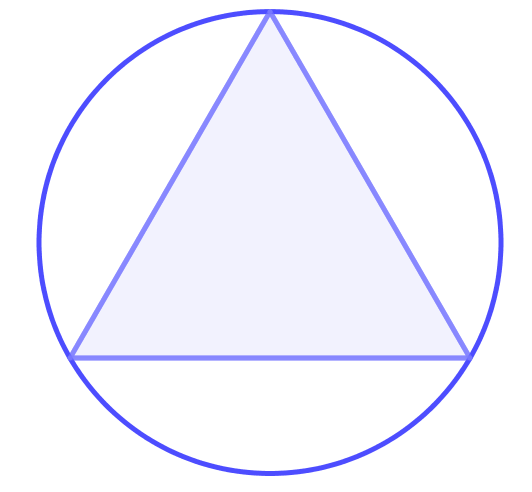
\includegraphics[width=.25\textwidth]{img-rt/rt42.png}
\end{figure}
	
\end{multicols}


\vspace{-6mm}
\begin{flushright}
\begin{footnotesize} \textcolor{gris}{\rotatebox{180}{ Dibuja radios. $\quad k=12$ }}	\end{footnotesize}
\end{flushright}

\item	Si $\ \tan x+\cot x=\pi\, , \ $ ¿qué vale $\ \sin x+\cos x \, $? 

\vspace{-6mm}
\begin{flushright}
\begin{footnotesize} \textcolor{gris}{\rotatebox{180}{ Escribe todo en función de senos y cosenos u opera. $\quad 1/\pi$ }}	\end{footnotesize}
\end{flushright}

\item ?`$\ (\cos x -\sin x)\, (\cos x+\sin x) = \cos^4 x - \sin^4 x\ $? 

\vspace{-6mm}
\begin{flushright}
\begin{footnotesize} \textcolor{gris}{\rotatebox{180}{ Sí }}	\end{footnotesize}
\end{flushright}


\item $\begin{cases} \ a\cos x+b\sin x= 3 \\ \ a\sin x-b\cos x=4 \end{cases} \quad$ ?`Qué vale $\ a^2+b^2 \ $?

\vspace{-6mm}
\begin{flushright}
\begin{footnotesize} \textcolor{gris}{\rotatebox{180}{ Eleva al cuadrado y suma, $\qquad 25$ }}	\end{footnotesize}
\end{flushright}


\item	Calcula: $\quad a)\ \cos 1^o+\cos 2^o+\cos 3^o+ \cdots + \cos 179^o \, ; \qquad b) \ \tan 1^o \cdot \tan 2^o \cdot \tan 3^o \cdot \cdots \cdot \tan 89^o$

$c)\ \ \ln \tan 1^o +\ln  \tan 2^o +\ln \tan 3^o + \cdots +\ln \tan 89^o$

\vspace{-6mm}
\begin{flushright}
\begin{footnotesize} \textcolor{gris}{\rotatebox{180}{ a) 0 (suplementarios); b) 1 (complementarios); $\quad$ c) 0 }}	\end{footnotesize}
\end{flushright}


\item	La ecuación $\ \sin^2 x+3\sin x \cos x+2\cos^2 x=0\, , \ $ ?`cuántas soluciones tiene en $[0,\pi[\, $?

\vspace{-6mm}
\begin{flushright}
\begin{footnotesize} \textcolor{gris}{\rotatebox{180}{ Saca $(\sin x+\cos x)$ factor común. Hay dos soluciones, $135^o$ y $153.4^o$ }}	\end{footnotesize}
\end{flushright}

\item	Simplifica $\quad \dfrac{\sin (90+x)\, \cot(90+x)º, \sin(270-x)}{\cos(180-x)\, \cos(90+x)}$

\vspace{-4mm}
\begin{flushright}
\begin{footnotesize} \textcolor{gris}{\rotatebox{180}{ Supon $x\in I.$cuadrante y relaciona todas las RT con él.$\quad$ Sol: $\ \sin x$ }}	\end{footnotesize}
\end{flushright}

\end{enumerate}




%********************************************************************
\vspace{1cm}
\section{Resumen del tema}

\begin{tikzpicture}
	\fill [left color=red!50, right color=teal!50] (0,0) rectangle (3.5,.1);
	\fill [left color=teal!50, right color=blue!50] (3.5,0) rectangle (7.5,.1);
	\end{tikzpicture}
\vspace{0.5cm}

\begin{myblock}{Resumen \emph{``Razones trigonométricas''}}
\begin{figure}[H]
	\centering
	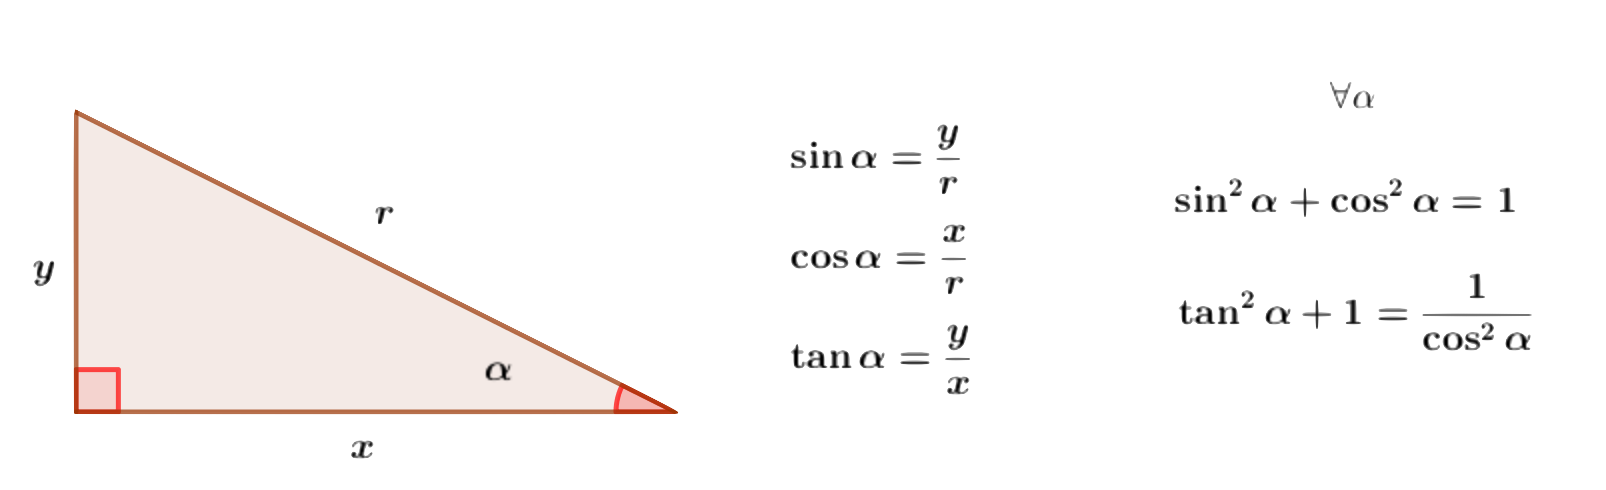
\includegraphics[width=1\textwidth]{img-rt/rt40.png}
\end{figure}	

\begin{table}[H]
\centering
\begin{tabular}{l|c|c|c|c|c|}
\cline{2-6}
 & $0^o$ & $30^o$ & $45^o$ & $60^o$ & $90^0$ \\ \hline
\multicolumn{1}{|l|}{$\sin \alpha$}  & $0$ & $1/2$ & $\sqrt{2}/2$ & $\sqrt{3}/2$ & $1$ \\ \hline
\multicolumn{1}{|l|}{$\cos \alpha$} & $1$ & $\sqrt{3}/2$ & $\sqrt{2}/2$ & $1/2$ & $0$ \\ \hline
\multicolumn{1}{|l|}{$\tan \alpha$} & $0$ & $\sqrt{3}/3$ & $1$ & $\sqrt{3}$ & $\nexists$ \\ \hline
\end{tabular}
\end{table}

\begin {itemize}
\vspace{-2mm}\item Ángulos con el mismo seno: $\alpha+\beta=180^o$ \hfill   \emph{(suplementarios)}
\vspace{-2mm}\item Ángulos con el mismo coseno $\alpha+\beta=360^o$ \hfill  \emph{(opuestos)}
\vspace{-2mm}\item Ángulos con la misma tangente: $\alpha-\beta=180^o$ \hfill  \emph{(se diferencian en 180$^o$)}
\vspace{-2mm}\item Ángulos que intercambian seno por coseno: $\alpha+\beta=90^o$ \hfill  \emph{(complementarios)}
\end {itemize}

\begin{figure}[H]
	\centering
	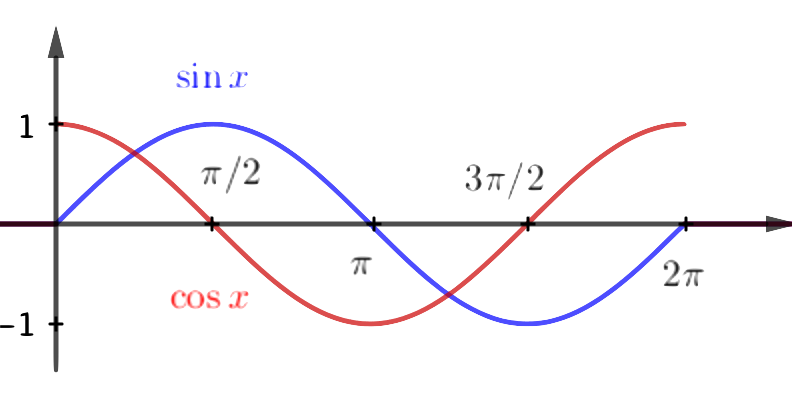
\includegraphics[width=.6\textwidth]{img-rt/rt39.png}
\end{figure}	
\end{myblock}












\begin{comment}

%%%%%%%%%%%%%%%%%%%%%%%%%%%%%%%%%%%. SECCIONES

\begin{figure}[H]
	\centering
	\includegraphics[width=0.35\textwidth]{img-pol/pol05.png}
\end{figure}


\chapter{texto}

\begin{tikzpicture}
	\fill [left color=red!50, right color=teal!50] (0,0) rectangle (6.5,.2);
	\fill [left color=teal!50, right color=blue!50] (6.5,0) rectangle (11.5,.2);
	\end{tikzpicture}

\vspace{1cm}
\section{texto}

\begin{tikzpicture}
	\fill [left color=red!50, right color=teal!50] (0,0) rectangle (3.5,.1);
	\fill [left color=teal!50, right color=blue!50] (3.5,0) rectangle (7.5,.1);
	\end{tikzpicture}
\vspace{0.5cm}

\subsection{texto}
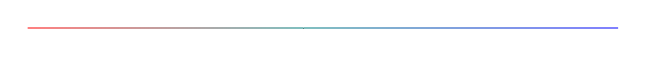
\begin{tikzpicture}
	\fill [left color=red!50, right color=teal!50] (0,0) rectangle (3.5,.01);
	\fill [left color=teal!50, right color=blue!50] (3.5,0) rectangle (7.5,.01);
	\end{tikzpicture}
\vspace{0.5cm}


%%%%%%%%%%%%%%%%%%%%%%%%%%%%%%%%%%%. \begin{ ------>. 
detsacado;  cuadro-naranja;  cuadro-gris;  miejercicio (solución extensa);  mipropuesto (solución corta y fuera del cuadro)

%%%%%%%%%%%%%%%%%%%%%%%%%%%%%%%%%%%. CURIOSIDAD
\vspace{1cm}
\color{ForestGreen!80}
\rule{250pt}{0.2pt}
Texto
\vspace{-8mm}
\begin{flushright}
\rule{250pt}{0.2pt}		
\end{flushright}	
\color{black}
\end{comment}